\documentclass[10pt]{article}
\usepackage[T1]{fontenc}
\usepackage{amsmath,amssymb,amsthm}
\usepackage[shortlabels]{enumitem}
\usepackage[english]{babel}
\usepackage[utf8]{inputenc}
\usepackage{fancyhdr}
\usepackage{bold-extra}
\usepackage{color}   
\usepackage{tocloft}
\usepackage{graphicx}
\usepackage{lipsum}
\usepackage{wrapfig}
\usepackage{cutwin}
\usepackage{hyperref}
\usepackage{lastpage}
\usepackage{multicol}
\usepackage{tikz}
\usepackage{xcolor}

% some useful math commands
\newcommand{\eps}{\varepsilon}
\newcommand{\R}{\mathbb{R}}
\newcommand{\C}{\mathbb{C}}
\newcommand{\N}{\mathbb{N}}
\newcommand{\Z}{\mathbb{Z}}
\newcommand{\Q}{\mathbb{Q}}
\newcommand{\K}{\mathbb{K}}
\newcommand{\F}{\mathbb{F}}
\newcommand{\norm}{\triangleleft}

\DeclareMathOperator{\Frac}{Frac}
\DeclareMathOperator{\Aut}{Aut}
\DeclareMathOperator{\im}{im}
\DeclareMathOperator{\ch}{ch}
\DeclareMathOperator{\Sub}{Sub}
\DeclareMathOperator{\Gal}{Gal}
\DeclareMathOperator{\Int}{Int}
\DeclareMathOperator{\id}{id}

\makeatletter
\renewcommand{\pod}[1]{\allowbreak\mathchoice
  {\if@display \mkern 18mu\else \mkern 8mu\fi (#1)}
  {\if@display \mkern 18mu\else \mkern 8mu\fi (#1)}
  {\mkern4mu(#1)}
  {\mkern4mu(#1)}
}

% title formatting
\newcommand{\newtitle}[4]{
  \begin{center}
	\huge{\textbf{\textsc{#1 Course Notes}}}
    
	\large{\sc #2}
    
	{\sc #3 \textbullet\, #4 \textbullet\, University of Waterloo}
	\normalsize\vspace{1cm}\hrule
  \end{center}
}

% for theorems
\newtheoremstyle{newstyle}      
{} %Aboveskip 
{-0.25pt} %Below skip
{\mdseries} %Body font e.g.\mdseries,\bfseries,\scshape,\itshape
{} %Indent
{\scshape} %Head font e.g.\bfseries,\scshape,\itshape
{.} %Punctuation afer theorem header
{ } %Space after theorem header
{} %Heading

\theoremstyle{newstyle}

\newtheorem*{prop*}{Proposition}
\newtheorem*{cor*}{Corollary}
\newtheorem*{exercise*}{Exercise}
\newtheorem*{lemma*}{Lemma}
\newtheorem*{remark*}{Remark}
\newtheorem*{exmp*}{Example}
\newtheorem*{defn*}{Definition}
\newtheorem*{thm*}{Theorem}
\newtheorem*{notation*}{Notation}
\newtheorem{thm}{Theorem}[section]
\newtheorem{fact}[thm]{Fact}
\newtheorem{cor}[thm]{Corollary}
\newtheorem{lemma}[thm]{Lemma}
\newtheorem{remark}[thm]{Remark}
\newtheorem{prop}[thm]{Proposition}
\newtheorem{defn}[thm]{Definition}
\newtheorem{claim}[thm]{Claim}
\newtheorem{axiom}[thm]{Axiom}
\newtheorem{notation}[thm]{Notation}
\newtheorem{exercise}[thm]{Exercise}
\newtheorem{exmp}[thm]{Example}

% new proof environment
\makeatletter
\newenvironment{pf}[1][\proofname]{\par
  \pushQED{\qed}%
  \normalfont \topsep0\p@\relax
  \trivlist
  \item[\hskip\labelsep\scshape
  #1\@addpunct{.}]\ignorespaces
}{%
  \popQED\endtrivlist\@endpefalse
}
\makeatother

% 1-inch margins
\topmargin 0pt
\advance \topmargin by -\headheight
\advance \topmargin by -\headsep
\textheight 8.9in
\oddsidemargin 0pt
\evensidemargin \oddsidemargin
\marginparwidth 0.5in
\textwidth 6.5in

% \renewcommand{\headrulewidth}{0pt}
% \renewcommand{\footrulewidth}{0.4pt}

\parindent 0in
\parskip 1.5ex

\setlist[itemize]{topsep=0pt}
\setlist[enumerate]{topsep=0pt}

% hyperlinks
\hypersetup{
  colorlinks=true, 
  linktoc=all,     % table of contents is clickable  
  allcolors=black  % all hyperlink colours
}

% table of contents
\addto\captionsenglish{
  \renewcommand{\contentsname}%
    {Table of Contents}%
}
\renewcommand{\cftsecfont}{\normalfont}
\renewcommand{\cftsecpagefont}{\normalfont}
\cftsetindents{section}{0em}{2em}

\fancypagestyle{plain}{%
\fancyhf{} % clear all header and footer fields
\lhead{PMATH 348: Winter 2021}
\fancyhead[R]{Table of Contents}
%\headrule
\fancyfoot[R]{{\small Page \thepage\ of \pageref*{LastPage}}}
}

% headers and footers
\pagestyle{fancy}
\renewcommand{\sectionmark}[1]{\markboth{#1}{#1}}
\lhead{PMATH 348: Winter 2021}
\cfoot{}
\setlength\headheight{14pt}

\setcounter{section}{-1}

\begin{document}

\pagestyle{fancy}
\newtitle{PMATH 348}{Fields and Galois Theory}{Yu-Ru Liu}{Winter 2021}
\rhead{Table of Contents}
\rfoot{{\small Page \thepage\ of \pageref*{LastPage}}}

\tableofcontents
\vspace{1cm}\hrule
\fancyhead[R]{\nouppercase\rightmark}
\newpage 
\fancyhead[R]{Week \thesection: \leftmark}

\section{Introduction}

We consider some types of polynomial equations. First, we introduce the notion of a radical.

\begin{defn}
An expression involving only $+, -, \times, \div, \sqrt[n]{}$ is called a {\bf radical}.
\end{defn}

{\bf Linear equations.} Let $ax + b = 0$ with $a, b \in \R$ and $a \neq 0$. The solution is $x = -b/a$.

{\bf Quadratic equations.} Let $ax^2 + bx + c = 0$ with $a, b, c \in \R$ and $a \neq 0$. The solutions are 
\[ x = \frac{-b \pm \sqrt{b^2-4ac}}{2a}. \]

{\bf Cubic equations.} A cubic equation can be reduced to an equation of the form 
\[ x^3 + px = q. \]
By Cardano's formula, a solution of the above equation is of the form 
\[ x = \sqrt[3]{\frac{q}2 + \sqrt{\frac{p^3}{27} + \frac{q^2}4}} + 
\sqrt[3]{\frac{q}2 - \sqrt{\frac{p^3}{27} + \frac{q^2}4}}. \]

{\bf Quartic equations.} Given a quartic equation, we can reduce it to a cubic equation, so 
solutions of quartic equations can also be expressed radically. 

{\bf Quintic equations.} This question was attempted by Euler, B\'ezout, and Lagrange without success.
In 1799, Ruffini gave an over 500-page proof about the insolvability of quintic equations; 
however, there was a small hole in his proof. In 1824, Abel filled in the gap in Ruffini's proof 
and completed the proof of the Abel-Ruffini theorem.

However, we can still ask the following question: given a {\it specific} quintic equation, is it 
solvable by radicals? 

Galois theory reverses this question. Suppose that a radical solution exists. 
What does its associated quintic equation look like?

{\bf Two main steps of Galois theory.}
\begin{enumerate}[(1)]
    \item Link a root of a quintic equation, $\alpha$, to $\Q(\alpha)$, the smallest field 
    containing $\Q$ and $\alpha$.
    \begin{itemize}
        \item Since $\Q(\alpha)$ is a field, it has more structures to play around with than $\alpha$.
        \item However, our knowledge about $\Q(\alpha)$ is still limited. For example, we do not 
        know how many intermediate fields $E$ there are between $\Q$ and $\Q(\alpha)$; that is, 
        $\Q \subseteq E \subseteq \Q(\alpha)$. For instance, we can think of many 
        examples of fields between $\Q$ and $\Q(\sqrt2, \sqrt3)$, such as 
        \[ \Q \subseteq \Q(\sqrt2), \Q(\sqrt3), \Q(\sqrt2+\sqrt3), \Q(\sqrt2-\sqrt3), \cdots 
        \subseteq \Q(\sqrt2, \sqrt3) \]
        by taking linear combinations of $\sqrt2$ and $\sqrt3$.
    \end{itemize}
    \item Link the field $\Q(\alpha)$ to a group. More precisely, we associate the field extension 
    $\Q(\alpha)/\Q$ to the automorphism group 
    \[ \Aut_{\Q}(\Q(\alpha)) = \{\phi : \Q(\alpha) \to \Q(\alpha) \text{ an isomorphism and fixes 
    $\Q$ pointwise}\}. \]
    \begin{itemize}
        \item If $\alpha$ is {\bf algebraic}, then $\Aut_{\Q}(\Q(\alpha))$ is finite. 
        \item If $\alpha$ is {\bf constructible}, then $\lvert\Aut_{\Q}(\Q(\alpha))\rvert$ is in certain
        forms.
        \item There is a bijective correspondence between the intermediate fields of 
        $\Q(\alpha)/\Q$ and the subgroups of $\Aut_{\Q}(\Q(\alpha))$.
    \end{itemize}
\end{enumerate}

{\bf Galois theory.} An interplay between fields and groups. In particular, it transforms an infinite 
field question into a finite group problem.

\section{Ring theory, Eisenstein's criterion}

\subsection{Review of ring theory}

We first review the ring theory that we need in this course. 

\begin{defn}
A {\bf commutative ring with unity} is a set $R$ equipped with addition ($+$) and 
multiplication ($\cdot$) such that
\begin{itemize}
    \item $R$ is an abelian group under addition with identity $0$;
    \item multiplication is commutative and associative;
    \item there exists an element $1 \in R$ such that $1 \cdot r = r$ for all $r \in R$; and 
    \item for all $r, s, t \in R$, we have $r(s+t) = rs+rt$.
\end{itemize}
\end{defn}

We will use the word {\bf ring} to refer to a commutative ring with unity. 

\begin{defn}
A {\bf field} $F$ is a ring in which every $a \in F \setminus \{0\}$ is a unit; 
that is, for all $a \in F \setminus \{0\}$, there exists $b \in F$ such that $ab = 1$. 
\end{defn}

\begin{defn}
A ring $R$ is an {\bf integral domain} if for all $a, b \in R$, $ab = 0$ implies that 
$a = 0$ or $b = 0$. 
\end{defn}

\begin{exmp}
The set of integers $\Z$ is an integral domain. The sets $\Q$, $\R$, $\C$, and $\Z_p$ 
(the congruence class modulo a prime $p$) are all fields.
\end{exmp}

\begin{prop}
Every subring of a field is an integral domain.
\end{prop}
\begin{pf}
Let $S \subseteq F$ be a subring of $F$, where $F$ is a field. Let $x, y \in S$. If $xy = 0$ 
in $S$, then $xy = 0$ in $F$ as well, so $x = 0$ or $y = 0$ (as $F$ is a field).
\end{pf}

\begin{defn}
An {\bf ideal} of a ring $R$ is a subset $I$ containing $0$ such that for all $a, b \in I$ and 
$r \in R$, we have $a - b \in I$ and $ra \in I$.
\end{defn}

\begin{exmp}
The only ideals of a field $F$ are $\{0\}$ and $F$. To see this, note that if $I$ is a non-zero 
ideal, then it contains some non-zero element, which is a unit as $R$ is a field.
\end{exmp}

\begin{defn}
An integral domain $R$ is a {\bf principal ideal domain (PID)} if every ideal is generated by 
a single element.
\end{defn}

In the following examples, we will see some similarities between $\Z$ and $F[x]$, where $F$ is a field.

\begin{exmp}
Consider the set of integers $\Z$. 
\begin{itemize}
    \item It is clear that $\Z$ is an integral domain with units $\{\pm1\}$. 
    \item Recall that the division algorithm in $\Z$ states that if $a, b \in \Z$ and $a \neq 0$, 
    then we can write $b = qa + r$ where $q, r \in \Z$ and $0 \leq r < |a|$.
    \item Using the division algorithm in $\Z$, we can show that every ideal $I$ of $\Z$ is 
    of the form $I = \langle n \rangle = n\Z$, so $\Z$ is a PID. Note that if 
    $n > 0$, then the generator $n$ is unique.
    \item Consider all fields containing $\Z$. Their intersection (the smallest field containing $\Z$) 
    is the set of rational numbers 
    \[ \Q = \left\{ \frac{a}b : a, b \in \Z \text{ and } b \neq 0 \right\}. \]
\end{itemize}
\end{exmp}

\begin{exmp}
Let $F$ be a field. We define 
\[ F[x] := \{f(x) = a_0 + a_1x + \cdots + a_mx^m : a_i \in F,\, 0 \leq i \leq m\}. \]
\begin{itemize}
    \item Recall that if $a_m = 1$, then $f(x)$ is said to be {\bf monic}. If $a_m \neq 0$, 
    the {\bf degree} of $f(x)$, written $\deg(f)$, is $m$. We also define $\deg(0) := -\infty$. 
    For any $f(x), g(x) \in F[x]$, we have that $\deg(fg) = \deg(f) + \deg(g)$.
    \item The set $F[x]$ is an integral domain with units $F^* = F \setminus \{0\}$. 
    \item The division algorithm in $F[x]$ states that for any $f(x), g(x) \in F[x]$ with 
    $f(x) \neq 0$, we can write $g(x) = q(x)f(x) + r(x)$, where $q(x), r(x) \in F[x]$ and 
    $\deg(r) < \deg(f)$.
    \item Using the division algorithm in $F[x]$, we can prove that every ideal $I$ of $F[x]$ 
    is of the form $I = \langle f(x) \rangle = f(x) F[x]$, so $F[x]$ is a PID. Note that if 
    the generator $f(x)$ is monic, then it is unique.
    \item Consider all fields containing $F[x]$. Their intersection (the smallest field containing 
    $F[x]$) is the set of rational functions 
    \[ F(x) = \left\{ \frac{f(x)}{g(x)} : f(x), g(x) \in F[x] \text{ and } g(x) \neq 0 \right\}. \]
\end{itemize}
\end{exmp}

\begin{defn}
Let $R$ be a ring and $I$ be an ideal of $R$. The {\bf quotient ring of $R$ modulo $I$}, 
denoted $R/I$, consists of elements of the form $r + I = \{r+s : s \in I\}$ where $r \in R$. 
Addition and multiplication in $R/I$ are defined by 
$(r_1 + I) + (r_2 + I) = (r_1 + r_2) + I$ and $(r_1 + I) \cdot (r_2 + I) = r_1r_2 + I$.
\end{defn}

\begin{exmp}
For $n \in \Z$, we have 
\[ \Z/\langle n \rangle = \{r = r + \langle n \rangle : 0 \leq r < |n|\}. \]
On the other hand, for $f(x) \in F[x]$, we have 
\[ F[x]/\langle f(x) \rangle = \{r(x) = r(x) + \langle f(x) \rangle : r(x) \in F[x],\, 
\deg(r) < \deg(f)\}. \]
\end{exmp}

\begin{thm}[First isomorphism theorem]
Let $\phi : R \to S$ be a ring homomorphism. Then the kernel of $\phi$, $\ker\phi =: I$, is an ideal. 
Moreover, there is a ring isomorphism $\psi : R/I \to \im\phi$ such that 
$\phi = \psi \circ q$, where $q : R \to R/I : r \mapsto r + I$ is the quotient homomorphism.
In other words, $\psi$ is the isomorphism 
\[ R/I \to \im\phi : r+I \mapsto \phi(r). \]
\end{thm}

\begin{exmp}
Let $F$ be a field and $S$ be a ring. Let $\phi : F \to S$ be a ring homomorphism. Since the 
only ideals of $F$ are $\{0\}$ and $F$, it follows that either $\phi$ is injective or $\phi = 0$.
\end{exmp}

\begin{defn}
An ideal $I$ in a ring $R$ is {\bf maximal} if $I \neq R$ and there is no ideal $J$ 
such that $I \subsetneq J \subsetneq R$.
\end{defn}

\begin{defn}
An ideal $I$ in a ring $R$ is {\bf prime} if $I \neq R$ and $ab \in I$ implies that $a \in I$ 
or $b \in I$.
\end{defn}

\begin{prop}
Every maximal ideal is prime. Moreover, in a PID, every prime ideal is maximal.
\end{prop}

\begin{exmp}
In $\Z$, $\langle n \rangle$ is maximal if and only if $n$ is prime. In $F[x]$, $\langle f(x) \rangle$ 
is maximal if and only if $f(x)$ is irreducible.
\end{exmp}

\begin{thm}
Let $I$ be an ideal of a ring $R$ and suppose $I \neq R$.
\begin{enumerate}[(1)]
    \item $I$ is maximal if and only if $R/I$ is a field.
    \item $I$ is prime if and only if $R/I$ is an integral domain.
\end{enumerate}
\end{thm}

\subsection{Eisenstein's criterion}

In this section, we apply Gauss' lemma (which was proved in PMATH 347) to prove Eisenstein's criterion.

\begin{lemma}[Gauss' lemma for $\Z [x{]}$]
Let $f(x) \in \Z[x]$ with $\deg(f) \geq 1$. If $f(x)$ is irreducible in $\Z[x]$, then $f(x)$ is 
also irreducible in $\Q[x]$.
\end{lemma}

\begin{remark}
The converse of the above is not true. Consider the polynomial $2x+8$, which is reducible 
in $\Z[x]$ since $2x+8 = 2(x+4)$ and we know that $2$ and $x+4$ are both non-units in $\Z[x]$. 
On the other hand, $2$ is a unit in $\Q[x]$, and hence $2x+8$ is irreducible in $\Q[x]$ 
(in fact, every degree $1$ polynomial is irreducible in $\Q[x]$ by this argument).
\end{remark}

\begin{thm}[Eisenstein's criterion for $\Z[x{]}$]
Let $f(x) = a_n x^n + a_{n-1} x^{n-1} + \cdots + a_0 \in \Z[x]$ with $n \geq 1$. 
Let $p \in \Z$ be prime and suppose that
\begin{itemize}
    \item $p \nmid a_n$;
    \item $p \mid a_i$ for all $0 \leq i \leq n-1$; and 
    \item $p^2 \nmid a_0$.
\end{itemize}
Then $f(x)$ is irreducible in $\Q[x]$.
\end{thm}
\begin{pf}
Consider the map $\Z[x] \to \Z_p[x]$ defined by 
\[ f(x) \mapsto \overline{f}(x) = \overline{a_n}x^n + \overline{a_{n-1}}x^{n-1} + \cdots + \overline{a_0}
\pmod p, \]
where for each $0 \leq i \leq n$ we have $\overline{a_i} \in \Z_p$ with $\overline{a_i} 
\equiv a_i \, (\text{mod } p)$. Since $p \nmid a_n$ and $p \mid a_i$ for all $0 \leq i \leq n-1$, 
we obtain $\overline{f}(x) = \overline{a_n}x^n$ with $\overline{a_n} \neq 0$. If 
$f(x)$ is reducible in $\Q[x]$, then by Gauss' lemma in $\Z[x]$, $f(x)$ is reducible in $\Z[x]$
as well; that is, $f(x) = g(x)h(x)$ for some $g(x), h(x) \in \Z[x]$ with $\deg(g) \geq 1$ and 
$\deg(h) \geq 1$. It follows that $\overline{a_n}x^n = \overline{g}(x) \overline{h}(x)$. 
Now, since $\Z_p[x]$ is a UFD, we see that $\overline{g}(x) = bx^m$ and $\overline{h}(x) = cx^k$ 
for some $b, c \in \Z_p$. In particular, both $\overline{g}(x)$ and $\overline{h}(x)$ have a $0$ constant 
in $\Z_p$. Since the constants of both $g(x)$ and $h(x)$ are both divisible by $p$, this implies that 
$p^2 \mid a_0$, a contradiction. Thus, $f(x)$ must be irreducible in $\Q[x]$, as required.
\end{pf}

\begin{exmp}
The polynomial $2x^7 + 3x^4 + 6x^2 + 12$ is irreducible in $\Q[x]$, since we can apply Eisenstein's 
criterion with $p = 3$.
\end{exmp}

\begin{exmp}
Let $p$ be a prime, and let 
\[ \zeta_p = e^{2\pi i/p} = \cos(2\pi/p) + i\sin(2\pi/p) \]
be a $p$-th root of $1$. Observe that this is a root of the $p$-th cyclotomic polynomial 
\[ \Phi_p(x) = \frac{x^p-1}{x-1} = x^{p-1} + x^{p-2} + \cdots + x + 1. \]
Eisenstein's criterion does not imply the irreducibility of $\Phi_p(x)$ immediately. 
However, we may consider 
\[ \Phi_p(x+1) = \frac{(x+1)^p - 1}{x} = x^{p-1} + \binom{p}1 x^{p-2} + \binom{p}2 x^{p-3} 
+ \cdots + \binom{p}{p-2}x + \binom{p}{p-1} \in \Z[x]. \]
Since $p$ is prime, we have that $p \nmid 1$, $p \mid \binom{p}i$ for all $1 \leq i \leq p-1$, 
and $p^2 \nmid \binom{p}{p-1}$. Hence, by Eisenstein's criterion for $\Z[x]$, 
$\Phi_p(x+1)$ is irreducible in $\Q[x]$. This implies that $\Phi_p(x)$ is irreducible in $\Q[x]$ 
as well; otherwise, there would exist $f(x), g(x) \in \Q[x]$ such that 
$\Phi_p(x) = f(x)g(x)$, but then this would imply that $\Phi_p(x+1) = f(x+1)g(x+1)$ is reducible
in $\Q[x]$, a contradiction. Since $\Phi_p(x)$ is primitive, it follows that $\Phi_p(x)$ is 
also irreducible in $\Z[x]$.
\end{exmp}

We can generalize the above results to PIDs.

\begin{lemma}[Gauss' lemma for PIDs]
Let $R$ be a PID and let $F$ be its field of fractions. Let $g(x) \in R[x]$ with $\deg(g) \geq 1$.
If $g(x)$ is irreducible in $R[x]$, then $g(x)$ is irreducible in $F[x]$. 
\end{lemma}

Let $R$ be a PID and suppose $\ell \in R$ is irreducible. Then $R/\langle\ell\rangle$ is 
a field, and $R/\langle\ell\rangle[x]$ is a UFD. Applying the same proof as Theorem 1.22, 
we can obtain the following result.

\begin{thm}[Eisenstein's criterion for PIDs]
Let $R$ be a PID and let $F$ be its field of fractions. Let $g(x) = b_n x^n + 
b_{n-1} x^{n-1} + \cdots + b_1x + b_0 \in R[x]$ with $n \geq 1$. Let $\ell \in R$ be irreducible 
and suppose that
\begin{itemize}
    \item $\ell \nmid b_n$;
    \item $\ell \mid b_i$ for all $0 \leq i \leq n-1$; and 
    \item $\ell^2 \nmid b_0$.
\end{itemize}
Then $f(x)$ is irreducible in $F[x]$.
\end{thm}

We can also generalize the above results to UFDs, but we need to modify the proof slightly. 

\begin{lemma}[Gauss' lemma for UFDs]
Let $S$ be a UFD and let $E$ be its field of fractions. Let $h(x) \in S[x]$ with $\deg(h) \geq 1$.
If $h(x)$ is irreducible in $S[x]$, then $h(x)$ is irreducible in $E[x]$. 
\end{lemma}

\begin{thm}[Eisenstein's criterion for UFDs]
Let $S$ be a UFD and let $E$ be its field of fractions. Let $h(x) = c_n x^n + 
c_{n-1} x^{n-1} + \cdots + c_1x + c_0 \in S[x]$ with $n \geq 1$. Let $\ell \in S$ be irreducible 
and suppose that
\begin{itemize}
    \item $\ell \nmid c_n$;
    \item $\ell \mid c_i$ for all $0 \leq i \leq n-1$; and 
    \item $\ell^2 \nmid c_0$.
\end{itemize}
Then $h(x)$ is irreducible in $E[x]$.
\end{thm}
\begin{pf}
We argue by contradiction. Suppose that $h(x)$ is reducible in $E[x]$. Then by 
Gauss' lemma for UFDs, there exist $s(x), r(x) \in S[x]$ with $\deg(s) \geq 1$ and 
$\deg(r) \geq 1$ such that $h(x) = s(x)r(x)$. We write 
\begin{align*}
    s(x) &= a_0 + a_1x + \cdots + a_m x^m, \\
    r(x) &= b_0 + b_1x + \cdots + b_k x^k,
\end{align*}
where $1 \leq m, k < n$. Since $h(x) = s(x)r(x)$, we have 
\[ c_j = \sum_{i=0}^j a_i b_{j-i} \]
for all $1 \leq j \leq n$. Consider the constant term $c_0 = a_0 b_0$. Since 
$\ell \mid c_0$, we have that $\ell \mid a_0 b_0$. Since $\ell$ is irreducible, 
we either have $\ell \mid a_0$ or $\ell \mid b_0$. Without loss of generality, 
suppose that $\ell \mid a_0$. Since $\ell^2 \nmid c_0$, we see that 
$\ell \nmid b_0$. Now, consider the coefficient of $x$. Since $\ell \mid c_1$, we have 
$\ell \mid a_0b_1 + a_1b_0$. Then, $\ell \mid a_0$ implies that $\ell \mid a_1b_0$, and 
$\ell \nmid b_0$ implies that $\ell \mid a_1$. Repeating the above argument implies that 
$\ell \mid a_i$ for all $0 \leq i \leq m-1$ and $\ell \nmid a_m$. Finally, 
consider the reduction $\overline{h}(x) = \overline{s}(x) \overline{r}(x) \in 
S/\langle\ell\rangle[x]$. By the assumption of the coefficients of $h$, we get 
$\overline{h}(x) = \overline{c_n}x^n$. However, since $\overline{s}(x) = \overline{a_m}x^m$ 
and $\ell \nmid b_0$, we see that $\overline{s}(x) \overline{r}(x)$ contains the term 
$\overline{a_m b_0} x^m$, which leads to a contradiction. Thus, $h(x)$ is irreducible in $E[x]$.
\end{pf}

\newpage
\section{Field extensions}

This week, we study various aspects of field extensions. In particular, our focus is to understand
the difference between extensions generated by algebraic elements and transcendental elements.

\subsection{Degree of extensions}

\begin{defn}
Let $E$ be a field containing another field $F$. We say that $E$ is a {\bf field extension} 
of $F$, and we write $E/F$.
\end{defn}

Note that the notation $E/F$ is not used to denote a quotient ring, as the field $E$ has no ideals
other than $\{0\}$ and $E$.

Moreover, if $E/F$ is a field extension, then we can view $E$ as a vector space over $F$.

\begin{defn}
The dimension of $E$ over $F$ (viewed as a vector space) is called the {\bf degree} of $E$ over $F$, 
and is denoted by $[E : F]$. If $[E : F] < \infty$, we say that $E/F$ is a {\bf finite extension}. 
Otherwise, we say that $E/F$ is an {\bf infinite extension}.
\end{defn}

\begin{exmp}
Note that $\C \cong \R+\R i$ (where $i^2=-1$), and hence we have $[\C : \R] = 2$.
\end{exmp}

\begin{exmp}
Let $F$ be a field. 
Recall that $F[x]$ is the polynomial ring over $F$, and $F(x)$ is the field of fractions of 
$F[x]$. Then $[F(x) : F] = \infty$ since $\{1, x, x^2, \dots\}$ is linearly independent over $F$.
\end{exmp}

\begin{thm}
If $E/K$ and $K/F$ are finite field extensions, then $E/F$ is a finite field extension and 
\[ [E : F] = [E : K] \cdot [K : F]. \]
In particular, if $K$ is an intermediate field of a finite extension $E/F$, then 
$[K : F]$ divides $[E : F]$.
\end{thm}
\begin{pf}
Suppose that $[E : K] = m$ and $[K : F] = n$. Let $\{a_1, \dots, a_m\}$ be a basis of 
$E/K$ and $\{b_1, \dots, b_n\}$ be a basis of $K/F$. It suffices to show that 
${\cal B} = \{a_ib_j : 1 \leq i \leq m,\, 1 \leq j \leq n\}$ is a basis of $E/F$. 
First, we show that every element of $E$ is a linear combination of elements in ${\cal B}$ over $F$. 

Let $e \in E$. Since $\{a_1, \dots, a_m\}$ is a basis for $E/K$, we have that 
\[ e = \sum_{i=0}^m k_i a_i \]
for some $k_i \in K$. Now, $\{b_1, \dots, b_n\}$ is a basis for $K/F$, and hence 
\[ k_i = \sum_{j=1}^n c_{i,j} b_j \] 
where $c_{i,j} \in F$. In particular, we obtain 
\[ e = \sum_{i=1}^m \sum_{j=1}^n c_{i,j} b_j a_i. \]
Next, we show that ${\cal B}$ is linearly independent over $F$. Suppose that 
\[ \sum_{i=1}^m \sum_{j=1}^n c_{i,j} b_j a_i = 0 \] 
where each $c_{i,j} \in F$. Since $\sum_{j=1}^n c_{i,j} b_j \in K$ and 
$\{a_1, \dots, a_m\}$ is linearly independent over $K$, we have 
\[ \sum_{j=1}^n c_{i,j} b_j = 0. \] 
Similarly, since $\{b_1, \dots, b_n\}$ is linearly independent over $F$, we must have 
$c_{i,j} = 0$. Thus, ${\cal B}$ is a basis for $E/F$, and we have 
\[ [E : F] = [E : K] \cdot [K : F]. \]
This completes the proof.
\end{pf}

\subsection{Algebraic and transcendental extensions}

\begin{defn}
Let $E/F$ be a field extension and $\alpha \in E$. We say that $\alpha$ is {\bf algebraic} 
over $F$ if there exists $f(x) \in F[x] \setminus \{0\}$ such that $f(\alpha) = 0$. 
Otherwise, we say that $\alpha$ is {\bf transcendental} over $F$.
\end{defn}

\begin{exmp}
Note that $\frac{c}d$ (where $c, d \in \R$), $\sqrt{2}$, and $\sqrt2 + \sqrt{-2}$ are 
algebraic over $\Q$ (see Assignment 2), but $e$ (Hermite, 1873) and $\pi$ (Lindemann, 1882) 
are transcendental over $\Q$.
\end{exmp}

Let $E/F$ be a field extension and $\alpha \in E$. We denote by $F[\alpha]$ the smallest 
subring of $E$ which contains $F$ and $\alpha$. We denote by $F(\alpha)$ the smallest 
subfield of $E$ which contains $F$ and $\alpha$. For $\alpha, \beta \in E$, we also denote 
$F[\alpha, \beta]$ and $F(\alpha, \beta)$ similarly.

\begin{defn}
If $E = F(\alpha)$ for some $\alpha \in E$, we say that $E$ is a {\bf simple extension} of $F$.
\end{defn}

The degree of the simple extension $F(\alpha)/F$ is either finite or infinite. We will see that 
this depends on whether $\alpha$ is algebraic or transcendental.

\begin{defn}
Let $R$ and $R'$ be two rings containing a field $F$. A ring homomorphism $\psi : R \to R'$ 
is called an {\bf $F$-homomorphism} if $\psi$ fixes $F$ pointwise; that is, 
$\psi(a) = a$ for all $a \in F$.
\end{defn}

\begin{thm}
Let $E/F$ be a field extension and $\alpha \in E$. If $\alpha$ is transcendental over $F$, 
then 
\[ F[\alpha] \cong F[x] \text{ and } F(\alpha) \cong F(x). \]
In particular, $F[\alpha] \neq F(\alpha)$.
\end{thm}
\begin{pf}
Let $\psi : F(x) \to F(\alpha)$ be the unique $F$-homomorphism defined by $\psi(x) = \alpha$. 
Thus, for $f(x), g(x) \in F[x]$ where $g(x) \neq 0$, we have 
\[ \psi \left( \frac{f(x)}{g(x)} \right) = \frac{f(\alpha)}{g(\alpha)} \in F(\alpha). \]
Note that since $\alpha$ is transcendental, we have $g(\alpha) \neq 0$. 
Thus, $\psi$ is well-defined. Now, since $F(x)$ is a field and $\ker\psi$ is an ideal of $F(x)$, 
we either have that $\psi = 0$ or $\psi$ is injective. Since $\psi(x) = \alpha \neq 0$, 
we see that $\psi$ is injective. Also, since $F(x)$ is a field, $\im\psi$ contains a 
field generated by $F$ and $\alpha$; that is, $F(\alpha) \subseteq \im\psi$. 
Thus, $\im\psi = F(\alpha)$ and $\psi$ is surjective. It follows that $\psi$ is an isomorphism. 
Hence, $F[\alpha] \cong F[x]$ and $F(\alpha) \cong F(x)$.
\end{pf}

\begin{thm}
Let $E/F$ be a field extension and $\alpha \in E$. If $\alpha$ is algebraic over $F$, 
then there exists a unique monic irreducible polynomial $p(x) \in F[x]$ such that there exists
an $F$-isomorphism 
\[ \psi : F[x]/\langle p(x) \rangle \to F[\alpha] : x \mapsto \alpha. \]
In particular, we may conclude that $F[\alpha] = F(\alpha)$.
\end{thm}
\begin{pf}
We first note that since $\alpha$ is algebraic, the map in the proof of Theorem 2.10 given by 
\[ \frac{f(x)}{g(x)} \mapsto \frac{f(\alpha)}{g(\alpha)} \] 
is not well-defined, as there exists $0 \neq g(x) \in F[x]$ such that $g(\alpha) = 0$. 
Consider the unique $F$-homomorphism $\psi : F[x] \to F(\alpha)$ defined by 
$\psi(x) = \alpha$. Thus for $f(x) \in F[x]$, we have 
$\psi(f(x)) = f(\alpha) \in F[\alpha]$. Since $F[x]$ is a ring, we see that 
$\im\psi$ contains a ring generated by $F$ and $\alpha$; that is, 
$F[\alpha] \subseteq \im\psi$. Thus, $\im\psi = F[\alpha]$. Let 
\[ I = \ker\psi = \{f(x) \in F[x] : f(\alpha) = 0\}. \] 
Since $\alpha$ is algebraic, we have $I \neq \{0\}$. Moreover, by the First Isomorphism 
Theorem, $F[x]/I \cong \im\psi$, which is a subring of the field $F(\alpha)$. Thus, 
$F[x]/I$ is an integral domain and $I$ is a prime ideal. It follows that 
$I = \langle p(x) \rangle$ where $p(x) \in F[x]$ is irreducible. If we assume that $p(x)$ 
is monic, then it is unique. Hence 
\[ F[x]/\langle p(x) \rangle \cong F[\alpha]. \] 
Since $p(x)$ is irreducible, we know that $F[x]/\langle p(x) \rangle$ is a field. 
Thus, $F[\alpha]$ is also a field. Also, since $F(\alpha)$ is the smallest field 
containing $F[\alpha]$, we get $F[\alpha] = F(\alpha)$. This completes the proof.
\end{pf}

\begin{defn}
If $\alpha$ is algebraic over a field $F$, the unique monic irreducible polynomial from 
Theorem 2.11 is called the {\bf minimal polynomial of $\alpha$ over $F$}. 
From the proof of Theorem 2.11, we see that if $f(x) \in F[x]$ with $f(\alpha) = 0$, then 
$p(x) \mid f(x)$. 
\end{defn}

As a direct consequence of Theorem 2.10 and Theorem 2.11, we obtain the following result. 

\begin{thm}
Let $E/F$ be a field extension and $\alpha \in E$.
\begin{enumerate}[(1)]
    \item $\alpha$ is transcendental if and only if $[F(\alpha) : F] = \infty$. 
    \item $\alpha$ is algebraic if and only if $[F(\alpha) : F] < \infty$.
\end{enumerate}
Moreover, if $\alpha$ is algebraic and $p(x)$ is the minimal polynomial of $\alpha$ over $F$, 
then $[F(\alpha) : F] = \deg(p)$ and $\{1, \alpha, \alpha^2, \dots, \alpha^{\deg(p)-1}\}$ is 
a basis for $F(\alpha)/F$. 
\end{thm}
\begin{pf}
It suffices to prove the left-to-right direction for (1) and (2) (as the right-to-left
direction of (1) is the left-to-right direction of (2), and vice versa).
\begin{enumerate}[(1)]
    \item Suppose $\alpha$ is transcendental over $F$. By Theorem 2.10, we have $F(\alpha) 
    \cong F(x)$. In $F(x)$, note that the elements $\{1, x, x^2, \dots\}$ are linearly 
    independent over $F$, and so $[F(\alpha) : F] = \infty$. 
    \item Suppose $\alpha$ is algebraic over $F$. By Theorem 2.11, we have 
    $F(\alpha) \cong F[x]/\langle p(x) \rangle$ with the mapping $x \mapsto \alpha$. 
    Note that 
    \[ F[x]/\langle p(x) \rangle = \{r(x) \in F[x] : \deg(r) < \deg(p)\}. \]
    Thus, $\{1, x, x^2, \dots, x^{\deg(p)-1}\}$ forms a basis of $F[x]/\langle p(x) \rangle$.
    It follows that $[F(\alpha) : F] = \deg(p)$ and $\{1, x, x^2, \dots, x^{\deg(p)-1}\}$ 
    is a basis of $F(\alpha)$ over $F$. \qedhere
\end{enumerate}
\end{pf}

Due to Theorem 2.13, it makes sense why we call $[F(\alpha) : F]$ the degree of the field extension.

\begin{exmp}
Let $p \in \Z$ be prime and let $\zeta_p = \exp(2\pi i/p)$ be a $p$-th root of unity. 
We saw in Example 1.24 that $\zeta_p$ is a root of the $p$-th cyclotomic polynomial 
$\Phi_p(x)$, which is irreducible. Thus, by Theorem 2.13, $\Phi_p(x)$ is the minimal polynomial 
of $\zeta_p$ over $\Q$ and 
\[ [\Q(\zeta_p) : \Q] = p-1. \]
The field $\Q(\zeta_p)$ is called the {\bf $p$-th cyclotomic extension} of $\Q$.
\end{exmp}

\begin{thm}
Let $E/F$ be a field extension. If $[E : F] < \infty$, then there exist elements 
$\alpha_1, \dots, \alpha_n \in E$ such that 
\[ F \subsetneq F(\alpha_1) \subsetneq F(\alpha_1, \alpha_2) \subsetneq \cdots 
\subsetneq F(\alpha_1, \dots, \alpha_n) = E. \]
Thus, to understand a finite extension, it suffices to understand a finite simple extension.
\end{thm}
\begin{pf}
We proceed by induction on $[E : F]$. If $[E : F] = 1$, then $E = F$ and we are done. 
Suppose that $[E : F] > 1$ and the statement holds for all field extensions $E'/F'$ 
with $[E' : F'] < [E : F]$. Let $\alpha_1 \in E \setminus F$. By Theorem 2.5, we have 
\[ [E : F] = [E : F(\alpha_1)] \cdot [F(\alpha_1) : F]. \]
Since $[F(\alpha_1) : F] > 1$, we have $[E : F(\alpha_1)] < [E : F]$. By the inductive hypothesis, 
there exist elements $\alpha_2, \alpha_3, \dots, \alpha_n \in E$ such that 
\[ F(\alpha_1) \subsetneq F(\alpha_1)(\alpha_2) \subsetneq F(\alpha_1)(\alpha_2, 
\alpha_3) \subsetneq \cdots 
\subsetneq F(\alpha_1)(\alpha_2, \dots, \alpha_n) = F(\alpha_1, \dots, \alpha_n) = E. \]
Thus, we obtain 
$F \subsetneq F(\alpha_1) \subsetneq F(\alpha_1, \alpha_2) \subsetneq \cdots 
\subsetneq F(\alpha_1, \dots, \alpha_n) = E$,
which completes the induction.
\end{pf}

\begin{defn}
A field extension $E/F$ is {\bf algebraic} if every $\alpha \in E$ is algebraic over $F$. 
Otherwise, we say that $E/F$ is {\bf transcendental}.
\end{defn}

\begin{thm}
Let $E/F$ be a field extension. If $[E : F] < \infty$, then $E/F$ is algebraic.
\end{thm}
\begin{pf}
Suppose that $[E : F] = n$. For $\alpha \in E$, the elements $\{1, \alpha, \alpha^2, \dots, \alpha^n\}$
are not linearly independent over $F$. Thus, there exist elements $c_0, c_1, \dots, c_n \in F$, 
not all $0$, such that 
\[ \sum_{i=0}^n c_i\alpha^i = 0. \]
Hence, $\alpha$ is a root of the polynomial $\sum_{i=0}^n c_i x^i \in F[x]$, and so 
$\alpha$ is algebraic over $F$.
\end{pf}

\begin{thm}
Let $E/F$ be a field extension. Then 
\[ L = \{\alpha \in E : [F(\alpha) : F] < \infty\} \] 
is an intermediate field of $E/F$.
\end{thm}
\begin{pf}
If $\alpha, \beta \in L$, we need to show that $\alpha \pm \beta$, $\alpha\beta$, and 
$\frac\alpha\beta$ (if $\beta \neq 0$) are in $L$. By definition of $L$, we have 
$[F(\alpha) : F] < \infty$ and $[F(\beta) : F] < \infty$. Consider the field $F(\alpha, \beta)$. 
Note that the minimal polynomial of $\alpha$ over $F$, say $p(x) \in F[x]$, is 
also a polynomial over $F(\beta)$ (that is, $p(x) \in F(\beta)[x]$) such that 
$p(\alpha) = 0$. 
Since the minimal polynomial of $\alpha$ over $F(\beta)$ divides the minimal polynomial 
of $\alpha$ over $F$, we have $[F(\alpha, \beta) : F(\beta)] \leq [F(\alpha) : F]$. 
Combined with Theorem 2.5, we obtain 
\[ [F(\alpha, \beta) : F] = [F(\alpha, \beta) : F(\beta)] \cdot [F(\beta) : F] \leq 
[F(\alpha) : F] \cdot [F(\beta) : F] < \infty. \] 
Since $\alpha + \beta \in F(\alpha, \beta)$, it follows that
\[ [F(\alpha + \beta) : F] \leq [F(\alpha, \beta) : F] < \infty, \]
and so $\alpha + \beta \in L$. By an analogous argument, we have that 
$\alpha-\beta$, $\alpha\beta$, and $\frac\alpha\beta$ (if $\beta\neq0$) are in $L$. 
Thus, $L$ is a field.
\end{pf}

\begin{defn}
Let $E/F$ be a field extension. The set 
\[ L = \{\alpha \in E : [F(\alpha) : F] < \infty\} \] 
is called the {\bf algebraic closure} of $F$ in $E$.
\end{defn}

\begin{defn}
A field $F$ is {\bf algebraically closed} if for any algebraic extension $E/F$, we have $E = F$.
\end{defn}

\begin{exmp}
By the Fundamental Theorem of Algebra, $\C$ is algebraically closed. Moreover, $\C$ is 
the algebraic closure of $\R$ in $\C$, and we have $[\C : \R] = 2$.
\end{exmp}

\begin{exmp}
Let $\overline{\Q}$ be the algebraic closure of $\Q$ in $\C$; that is, 
\[ \overline{\Q} = \{\alpha \in \C : \alpha \text{ is algebraic over $\Q$}\}. \]
Since $\zeta_p \in \overline{\Q}$, we have 
\[ [\overline{\Q} : \Q] \geq [\Q(\zeta_p) : \Q] = p-1. \]
As there are infinitely many primes, we have $[\overline{\Q} : \Q] = \infty$. We saw in Theorem 
2.17 that if $E/F$ is finite, then $E/F$ is algebraic. However, this example shows that the 
converse is not true.
\end{exmp}

\newpage 
\section{Splitting fields}

This week, we introduce splitting fields and prove the existence and uniqueness of such fields.
We also give a bound for the degrees of such field extensions. 

\begin{defn}
Let $E/F$ be a field extension. We say that $f(x) \in F[x]$ {\bf splits over} $E$ if $E$ 
contains all roots of $f(x)$; that is, $f(x)$ is a product of linear factors in $E[x]$.
\end{defn}

\begin{defn}
Let $\widehat{E} / F$ be a field extension, $f(x) \in F[x]$, and $F \subseteq E \subseteq \widehat{E}$.
If 
\begin{enumerate}[(1)]
    \item $f(x)$ splits over $E$, and 
    \item there is no proper subfield of $E$ in which $f(x)$ splits over,
\end{enumerate}
then we say that $E$ is a {\bf splitting field of $f(x)$ over $\widehat{E}$}.
\end{defn}

\subsection{Existence of splitting fields}

To show that a splitting field of $f(x)$ exists, we first find a field extension of $F$ 
which contains at least one root of $f(x)$.

\begin{thm}
Let $p(x) \in F[x]$ be irreducible. The quotient ring $F[x]/\langle p(x) \rangle$ is a field 
containing $F$ and a root of $p(x)$.
\end{thm}
\begin{pf}
Since $p(x)$ is irreducible, the ideal $I = \langle p(x) \rangle$ is maximal. Thus, 
$E = F[x]/I$ is a field. Now, consider the map 
\[ \psi : F \to E : a \mapsto a + I. \]
Since $F$ is a field and $\psi \neq 0$, we see that $\psi$ is injective. Hence, by identifying 
$F$ with its image $\psi(F)$, we can view $F$ as a subfield of $E$. 

Let $\alpha = x + I \in E$. We claim that $\alpha$ is a root of $p(x)$. Indeed, we can write 
\begin{align*}
    p(x) &= a_0 + a_1x + \cdots + a_n x^n \\
    &= (a_0 + I) + (a_1 + I) + \cdots + (a_n + I)x^n \in E[x]. 
\end{align*}
Then, we have 
\begin{align*}
    p(\alpha) &= (a_0 + I) + (a_1 + I)\alpha + \cdots + (a_n + I)x^n \\
    &= (a_0 + I) + (a_1 + I)(x + I) + \cdots + (a_n + I)(x + I)^n \\
    &= (a_0 + a_1x + \cdots + a_n x^n) + I \\
    &= p(x) + I = 0 + I = I.
\end{align*}
Hence, $\alpha = x+I \in E$ is a root of $p(x)$.
\end{pf}

\begin{thm}[Kronecker]
Let $f(x) \in F[x]$. Then there exists a field $E$ containing $F$ such that $f(x)$ splits over $E$.
\end{thm}
\begin{pf}
We proceed by induction on $\deg(f)$. If $\deg(f) = 1$, we may simply let $E = F$ and we are done. 
Suppose that $\deg(f) > 1$, and the statement holds for all $g(x)$ with $\deg(g) < \deg(f)$ 
(with $g(x)$ not necessarily being in $F[x]$). Write $f(x) = p(x)h(x)$ where 
$p(x), h(x) \in F[x]$ and $p(x)$ is irreducible. By Theorem 3.3, there exists a field 
$F \subseteq K$ with $K$ containing a root of $p(x)$, say $\alpha$. Then 
for some $q \in K[x]$, we have $p(x) = (x - \alpha) q(x)$ and hence 
\[ f(x) = (x-\alpha) h(x) q(x). \]
Since $\deg(hq) < \deg(f)$, it follows by the inductive hypothesis that there exists a field 
$E$ containing $K$ over which $h(x)q(x)$ splits. Thus, $f(x)$ splits over $E$.
\end{pf}

\begin{thm}
Every $f(x) \in F[x]$ has a splitting field, which is a field extension of $F$. 
\end{thm}
\begin{pf}
For $f(x) \in F[x]$, we know by Theorem 3.4 that there exists a field extension $E/F$ 
over which $f(x)$ splits. Suppose that $\alpha_1, \dots, \alpha_n$ are the roots of $f(x)$ in $E$, 
and consider $F(\alpha_1, \dots, \alpha_n)$. This is the smallest subfield of $E$ containing all 
roots of $f(x)$, so $f(x)$ does not split over any proper subfield of it. Thus, 
$F(\alpha_1, \dots, \alpha_n)$ is the splitting field of $f(x)$ in $E$. Moreover, 
since $\alpha_1, \dots, \alpha_n$ are all algebraic, we see that 
$F(\alpha_1, \dots, \alpha_n)/F$ is a finite extension. 
\end{pf}

\subsection{Uniqueness of splitting fields}
Due to Theorem 3.5, we see that for a fixed field extension $E/F$, a splitting field 
of $f(x) \in F[x]$ in $E$ is of the form $F(\alpha_1, \dots, \alpha_n)$, where the 
$\alpha_i$ are the roots of $f(x)$ in $E$. Thus, it is unique within $E$. 

If we change $E/F$ to a different field extension, say $E_1/F$, what is the relationship 
between the splitting field of $f(x)$ in $E$ and the one in $E_1$?

\begin{defn}
Let $\phi : R \to R_1$ be a ring homomorphism, and $\Phi : R[x] \to R_1[x]$ be the unique 
ring homomorphism satisfying $\Phi|_R = \phi$ and $\Phi(x) = x$. In this case, we say that 
$\Phi$ {\bf extends} $\phi$. 
More generally, if $R \subseteq S$, $R_1 \subseteq S_1$, and $\Phi : S \to S_1$ is a ring 
homomorphism with $\Phi|_R = \phi$, we say that $\Phi$ {\bf extends} $\phi$.
\end{defn}

\begin{thm}
Let $\phi : F \to F_1$ be a field isomorphism and let $f(x) \in F[x]$. Let 
$\Phi : F[x] \to F_1[x]$ be the unique ring isomorphism which extends $\phi$ (as in Definition 3.6). 
Let $f_1(x) = \Phi(f(x))$, and let $E/F$ and $E_1/F_1$ be splitting fields of $f(x)$ and $f_1(x)$ 
respectively. Then there exists an isomorphism $\psi : E \to E_1$ which extends $\phi$. 
\end{thm}
\begin{pf}
We proceed by induction on $[E : F]$. If $[E : F] = 1$, then $f(x)$ is a product of linear factors 
in $F[x]$, and hence so is $f_1(x)$ in $F_1[x]$. Thus, $E = F$ and $E_1 = F_1$, so we may 
simply take $\psi = \phi$. 

Suppose $[E : F] > 1$ and suppose the statement is true for all field extensions 
$\widehat{E}/\widehat{F}$ with $[\widehat{E} : \widehat{F}] < [E : F]$. 
Let $p(x) \in F[x]$ be an irreducible factor of $f(x)$ with $\deg(p) \geq 2$, and let $p_1(x) 
= \Phi(p(x))$. We note that such a $p(x)$ exists because if all irreducible factors are of 
degree $1$, then $[E : F] = 1$. Now, let $\alpha \in E$ and $\alpha_1 \in E_1$ 
be roots of $p(x)$ and $p_1(x)$ respectively. By Theorem 2.11, we have an $F$-isomorphism 
\[ F(\alpha) \to F[x]/\langle p(x) \rangle : \alpha \mapsto x + \langle p(x) \rangle. \]
Similarly, there is an $F_1$-isomorphism 
\[ F_1(\alpha_1) \to F_1[x]/\langle p_1(x) \rangle : \alpha_1 \mapsto x + \langle p_1(x) \rangle. \]
Consider the isomorphism $\Phi : F[x] \to F_1[x]$ which extends $\phi$. Since 
$p_1(x) = \Phi(p(x))$, there exists a field isomorphism 
\[ \tilde{\Phi} : F[x]/\langle p(x) \rangle \to F_1[x]/\langle p_1(x) \rangle 
: x + \langle p(x) \rangle \mapsto x + \langle p_1(x) \rangle \]
which extends $\phi$. It follows that there is a field isomorphism 
\[ \tilde{\phi} : F(\alpha) \to F_1(\alpha_1) : \alpha \mapsto \alpha_1 \]
extending $\phi$. Note that since $\deg(p) \geq 2$, we have $[E : F(\alpha)] < [E : F]$. 
Since $E$ (respectively $E_1$) is the splitting field of $f(x) \in F(\alpha)[x]$ 
(respectively $f_1(x) \in F_1(\alpha_1)[x]$) over $F(\alpha)$ (respectively $F_1(\alpha_1)$), 
it follows by induction that there exists $\psi : E \to E_1$ which extends $\tilde\phi$. 
Thus, $\psi$ also extends $\phi$. 
\end{pf}

\begin{cor}
Any two splitting fields of $f(x) \in F[x]$ over $F$ are $F$-isomorphic.
\end{cor}
\begin{pf}
Let $\phi : F \to F$ be the identity map, and apply Theorem 3.7.
\end{pf}

Consequently, given $f(x) \in F[x]$, we can now refer to {\it the} splitting field of $f(x)$ over $F$. 

\subsection{Degrees of splitting fields}

\begin{thm}
Let $F$ be a field and let $f(x) \in F[x]$ with $\deg(f) = n \geq 1$. If $E/F$ is the 
splitting field of $f(x)$, then $[E : F] \mid n!$. 
\end{thm}
\begin{pf}
We proceed by induction on $\deg(f)$. If $\deg(f) = 1$, choose $E = F$ and we have 
$[E : F] \mid 1!$. Suppose $\deg(f) > 1$ and that the statement holds for all 
$g(x)$ with $\deg(g) < \deg(f)$ (where $g(x)$ is not necessarily in $F[x]$). 
We consider two cases. 
\begin{enumerate}[(1)]
    \item If $f(x) \in F[x]$ is irreducible and $\alpha \in E$ is a root of $f(x)$, then 
    by Theorem 2.11, $F(\alpha) \cong F[x]/\langle f(x) \rangle$ and $[F(\alpha) : F] = \deg(f) = n$. 
    Write $f(x) = (x-\alpha)g(x) \in F(\alpha)[x]$ with $g(x) \in F(\alpha)[x]$. Since $E$ is the 
    splitting field of $g(x)$ over $F(\alpha)$ and $\deg(g) = n-1$, it follows by induction that 
    $[E : F(\alpha)] \mid (n-1)!$. Since $[E : F] = [E : F(\alpha)] \cdot [F(\alpha) : F]$, 
    we obtain $[E : F] \mid n!$. 
    \item If $f(x)$ is not irreducible, we can write $f(x) = g(x)h(x)$ where $g(x), h(x) \in F[x]$ 
    with $\deg(g) = m$, $\deg(h) = k$, $m + k = n$, and $1 \leq m, k < n$. Let $K$ be the 
    splitting field of $g(x)$ over $F$. Since $\deg(g) = m$, it follows by 
    induction that $[K : F] \mid m!$. Similarly, since $E$ is the splitting field of $h(x)$ 
    over $K$ and $\deg(h) = k$, we have by induction that $[E : K] \mid k!$. Thus, 
    $[E : F] \mid m!k!$, which is a factor of $n!$ (since $\frac{n!}{m!k!} = \binom{n}{m} \in \Z$).
    \qedhere
\end{enumerate}
\end{pf}

\newpage 
\section{More field theory}

This week, we introduce some more field theory. Our focus to understand the differences between 
fields of characteristic $0$ and fields of characteristic $p$ (where $p$ is prime).

\subsection{Prime fields}

\begin{defn}
The {\bf prime field} of a field $F$ is the intersection of all subfields of $F$.
\end{defn}

\begin{thm}
If $F$ is a field, then its prime field is isomorphic to either $\Q$ or $\Z_p$ for 
some prime $p$.
\end{thm}
\begin{pf}
Let $F_1$ be a subfield of $F$. Consider the ring map 
\[ \chi : \Z \to F_1 : n \mapsto n \cdot 1 \]
where $1 \in F_1 \subseteq F$. Let $I = \ker\chi$ be the kernel of $\chi$. 
Since $\Z/I \cong \im\chi$ (by the First Isomorphism Theorem) which is a subring of 
$F_1$, it is an integral domain. Thus, $I$ is a prime ideal. We now consider two cases. 
\begin{itemize}
    \item If $I = \langle 0 \rangle$, then $\Z \subseteq F_1$. Since $F_1$ is a field, 
    we have 
    $\Q = \Frac(\Z) \subseteq F_1$. 
    \item If $I = \langle p \rangle$, it follows from the First Isomorphism Theorem that 
    $\Z_p = \Z/\langle p \rangle \cong \im\chi \subseteq F_1$. \qedhere 
\end{itemize}
\end{pf}

\begin{defn}
Let $F$ be a field. If the prime field of $F$ is isomorphic to $\Q$ (respectively $\Z_p$), 
we say that $F$ has {\bf characteristic} 0 (respectively {\bf characteristic} $p$), 
and we write $\ch(F) = 0$ (respectively $\ch(F) = p$).
\end{defn}

Note that if $\ch(F) = p$, then for all $a, b \in F$, we have $(a+b)^p = a^p + b^p$. 
Using this property, we get the following result. 

\begin{prop}
Let $F$ be a field with $\ch(F) = p$ and let $n \in \N$. Then the map $\varphi : F \to F 
: u \mapsto u^{p^n}$ is an injective $\Z_p$-homomorphism of fields. If $F$ is finite, then 
$\varphi$ is a $\Z_p$-isomorphism of $F$.
\end{prop}

\subsection{Formal derivatives and repeated roots}

\begin{defn}
If $F$ is a field, the monomials $\{1, x, x^2, \dots\}$ form an $F$-basis of $F[x]$. 
Define the linear operator $D : F[x] \to F[x]$ by $D(1) = 0$ and $D(x^i) = ix^{i-1}$ for 
all $i \in \N$. In particular, for $f(x) = a_0 + a_1x + a_2x^2 + \cdots + a_nx^n$ where 
each $a_i \in F$, we have 
\[ D(f)(x) = a_1 + 2a_2x + \cdots + na_n x^{n-1}. \]
Note that for all $f, g \in F[x]$, we have 
\begin{enumerate}[(1)]
    \item $D(f+g) = D(f) + D(g)$, and 
    \item $D(fg) = D(f) \cdot g + f \cdot D(g)$ (called the Leibniz rule).
\end{enumerate}
We call $D(f) = f'$ the {\bf formal derivative} of $f$.
\end{defn}

\begin{thm}
Let $F$ be a field and let $f(x) \in F[x]$. 
\begin{enumerate}[(a)]
    \item If $\ch(F) = 0$, then $f'(x) = 0$ if and only if $f(x) = c$ for some $c \in F$.
    \item If $\ch(F) = p$, then $f'(x) = 0$ if and only if $f(x) = g(x^p)$ for some 
    $g(x) \in F[x]$.
\end{enumerate}
\end{thm}
\begin{pf}~
\begin{enumerate}[(a)]
    \item $(\Leftarrow)$ This is clear. 
    
    $(\Rightarrow)$ Suppose that $f(x) = a_0 + a_1x + \cdots + a_nx^n$. Then 
    $f'(x) = a_1 + 2a_2x + \cdots + na_n x^{n-1} = 0$, and so $ia_i = 0$ for all 
    $1 \leq i \leq n$. Since $\ch(F) = 0$, we have $i \neq 0$, and hence $a_i = 0$ for all 
    $1 \leq i \leq n$. Thus, $f(x) = a_0$.
    
    \item $(\Leftarrow)$ Suppose that $f(x) = g(x^p)$ where $g(x) = b_0 + b_1x + \cdots + 
    b_m x^m \in F[x]$. Then 
    \[ f(x) = g(x^p) = b_0 + b_1 x^p + b_2 x^{2p} + \cdots + b_m x^{pm}. \]
    It follows that 
    \[ f'(x) = pb_1 x^{p-1} + 2pb_2 x^{2p-1} + \cdots + mpb_m x^{pm-1}. \]
    Since $\ch(F) = p$, we have $f'(x) = 0$. 
    
    $(\Rightarrow)$ Suppose that $f(x) = a_0 + a_1x + \cdots + a_n x^n$. Then 
    $f'(x) = a_1 + 2a_2x + \cdots + na_n x^{n-1} = 0$, which implies that 
    $ia_i = 0$ for all $1 \leq i \leq n$. Since $\ch(F) = p$, we see that $ia_i = 0$ implies $a_i = 0$ 
    unless $p \mid i$. Thus, we get 
    \[ f(x) = a_0 + a_p x^p + a_{2p} x^{2p} + \cdots + a_{mp} x^{mp} = g(x^p), \]
    where $g(x) = a_0 + a_p x + a_{2p} x^2 + \cdots + a_{mp} x^m \in F[x]$. \qedhere 
\end{enumerate}
\end{pf}

\begin{defn}
Let $E/F$ be a field extension and let $f(x) \in F[x]$. We say that $\alpha \in E$ is a {\bf repeated 
root} of $f(x)$ if $f(x) = (x - \alpha)^2 g(x)$ for some $g(x) \in E[x]$. 
\end{defn}

\begin{thm}
Let $E/F$ be a field extension, $f(x) \in F[x]$, and $\alpha \in E$. 
Then $\alpha$ is a repeated root of $f(x)$ if and only if $(x - \alpha)$ divides both 
$f$ and $f'$; that is, $(x-\alpha) \mid \gcd(f, f')$. 
\end{thm}
\begin{pf}
$(\Rightarrow)$ Suppose that $f(x) = (x-\alpha)^2 g(x)$ for some $g(x) \in E[x]$. 
Then 
\[ f'(x) = 2(x-\alpha) g(x) + (x-\alpha)^2 g'(x) = (x-\alpha) (2g(x) + (x-\alpha)g'(x)), \]
so $(x-\alpha)$ divides both $f$ and $f'$. 

$(\Leftarrow)$ Suppose that $(x - \alpha)$ divides both $f$ and $f'$. Write $f(x) = 
(x-\alpha) h(x)$ where $h(x) \in E[x]$. Then 
\[ f'(x) = h(x) + (x-\alpha) h'(x). \]
Since $f'(\alpha) = 0$, we have $h(\alpha) = 0$. Hence, $(x-\alpha)$ is a factor of $h(x)$ 
and $f(x) = (x-\alpha)^2 g(x)$ for some $g(x) \in E[x]$. 
\end{pf}

\begin{cor}
Let $F$ be a field and let $f(x) \in F[x]$. Then $f(x)$ has no repeated roots in any field extension of 
$F$ if and only if $\gcd(f, f') = 1$. 
\end{cor}
\begin{pf}
Note that $\gcd(f, f') \neq 1$ if and only if $(x-\alpha) \mid \gcd(f, f')$ for 
an element $\alpha$ in some extension of $F$. By Theorem 4.8, the result holds. 
\end{pf}

Observe that the condition of repeated roots depends on the extensions of $F$, 
whereas the gcd condition involves only $F$. 

\subsection{Finite fields}
Given a field $F$, we let $F^* = F \setminus \{0\}$ denote the multiplicative 
group of non-zero elements in $F$. 

\begin{prop}
If $F$ is a finite field, then $\ch(F) = p$ for some prime $p$, and 
$|F| = p^n$ for some $n \in \N$. 
\end{prop}
\begin{pf}
Since $F$ is a finite field, it follows from Theorem 4.2 that its prime field is $\Z_p$. 
Moreover, since $F$ is a finite dimensional vector space over $\Z_p$, we have $F \cong \Z_p^n$ 
for some $n \in \N$. Thus, $|F| = p^n$. 
\end{pf}

\begin{thm}
Let $F$ be a field and $G$ be a finite subgroup of $F^*$. Then $G$ is a cyclic group. 
In particular, if $F$ is a finite field, then $F^*$ is a cyclic group. 
\end{thm}
\begin{pf}
Without loss of generality, we can assume that $G \neq \{1\}$. Since $G$ is a 
finite abelian group, we have $G \cong \Z/n_1\Z \times \Z/n_2\Z \times \cdots \times 
\Z/n_r\Z$ where $n_1 > 1$ and $n_i \mid n_{i+1}$ for all $1 \leq i \leq r-1$. 
Since $n_r(\Z/n_1\Z \times \Z/n_2\Z \times \cdots \times \Z/n_r\Z) = 0$, it follows 
that every $u \in G$ is a root of $x^{n_r} - 1 \in F[x]$. Since this polynomial 
has at most $n_r$ distinct roots in $F$, we have $r = 1$ and $G \cong \Z/n_r\Z$.
\end{pf}

\begin{cor}
If $F$ is a finite field, then $F$ is a simple extension of $\Z_p$; that is, 
$F= \Z_p(u)$ for some $u \in F$.
\end{cor}
\begin{pf}
Take $u$ to be a generator of the multiplicative group $F^*$, which exists by Theorem 4.11.
\end{pf}

\begin{thm}
Let $p$ be prime and let $n \in \N$. 
\begin{enumerate}[(a)]
    \item $F$ is a finite field with $|F| = p^n$ if and only if $F$ is a splitting field 
    of $x^{p^n} - x$ over $\Z_p$. 
    \item Let $F$ be a finite field with $|F| = p^n$. Let $m \in \N$ such that 
    $m \mid n$. Then $F$ contains a unique subfield $K$ with $|K| = p^m$.
\end{enumerate}
\end{thm}
\begin{pf}~
\begin{enumerate}[(a)]
    \item $(\Rightarrow)$ If $|F| = p^n$, then $|F^*| = p^n - 1$. Then every $u \in F^*$ satisfies 
    $u^{p^n-1} = 1$, and hence is a root of $x(x^{p^n-1}-1) = x^{p^n} - x \in \Z_p[x]$. 
    Since $0 \in F$ is also a root of $x^{p^n} - x$, the polynomial $x^{p^n} - x$ 
    has $p^n$ distinct roots in $F$; that is, it splits over $F$. Thus, $F$ 
    is a splitting field of $x^{p^n} - x$ over $\Z_p$. 
    
    $(\Leftarrow)$ Suppose that $F$ is a splitting field of $f(x) = x^{p^n} - x$ over $\Z_p$. 
    Since $\ch(F) = p$, we have $f'(x) = -1$. Also, since $\gcd(f, f') = 1$, we have by 
    Corollary 4.9 that $f(x)$ has $p^n$ distinct roots in $F$. Let $E$ be the 
    set of all roots of $f(x)$ in $F$. Consider the mapping $\varphi : F \to F : u \mapsto u^{p^n}$. 
    If $u \in F$, then $u$ is a root of $f(x)$ if and only if $\varphi(u) = u$. 
    Since this condition is closed under addition, subtraction, multiplication, and 
    division, the set $E$ is a subfield of $F$ of order $p^n$ which contains $\Z_p$ 
    (since all $u \in \Z_p$ satisfy $u^p = u$ and hence $u^{p^n} = u$). Since $F$ is a 
    splitting field, it is generated by $\Z_p$ by the roots of $f(x)$; namely, the 
    elements of $E$. Thus, $F = \Z_p(E) = E$. 
    
    \item Recall that 
    \[ x^{ab} - 1 = (x^a - 1)(x^{ab-a} + x^{ab-2a} + \cdots + x^a + 1). \]
    Thus, if $n = mk$, then we have 
    \[ x^{p^n} - x = x(x^{p^n-1}-1) = x(x^{p^m-1}-1)g(x) = (x^{p^m}-x)g(x) \]
    for some $g(x) \in \Z_p[x]$. Since $x^{p^n}-x$ splits over $F$ by part (a), so does 
    $x^{p^m}-x$. Let 
    \[ K = \{u \in F : u^{p^n} - u = 0\}. \]
    Then $|K| = p^n$ since the roots of $x^{p^m} - x$ are distinct. Moreover, by part (a), 
    $K$ is a field. Note that if $\widetilde{K} \subseteq F$ is any subfield with 
    $|\widetilde{K}| = p^m$, then $\widetilde{K} \subseteq K$, so it follows that 
    $\widetilde{K} = K$. Thus, any subfield $K$ of $F$ such that $|K| = p^m$ is unique. \qedhere 
\end{enumerate}
\end{pf}

As a direct consequence of Theorem 4.13 and Corollary 3.8 (which states that any two splitting 
fields of $f(x) \in F[x]$ are isomorphic), we have the following result. 

\begin{cor}[E. H. Moore]
Let $p$ be prime and let $n \in \N$. Then any two finite fields of order $p^n$ are 
isomorphic. We denote such a field by $\mathbb{F}_{p^n}$. 
\end{cor}

\subsection{Separable polynomials}

\begin{defn}
Let $F$ be a field and let $f(x) \in F[x] \setminus \{0\}$. If $f(x)$ is irreducible, 
we say that $f(x)$ is {\bf separable over $F$} if it has no repeated root in 
any extension of $F$. On the other hand, if $f(x)$ is reducible, we say that 
$f(x)$ is separable over $F$ if each irreducible factor of $f(x)$ is separable 
over $F$. 
\end{defn}

\begin{exmp}
The polynomial $f(x) = (x-4)^9$ is separable over $\Q$. 
\end{exmp}

\begin{exmp}
Let $n \geq 2$ and consider the polynomial $f(x) = x^n - a \in F[x]$. Recall Corollary 4.9, 
which states that if $\gcd(f, f') = 1$, then $f(x)$ has no repeated root in any extension of $F$;
in particular, $f(x)$ is separable over $F$. 

Note that if $a = 0$, the only irreducible factor of $f(x)$ is $x$. Since $\gcd(x, x') = 1$, 
we see that $f(x)$ is separable. 

Now, assume that $a \neq 0$. Note that $f'(x) = nx^{n-1}$, and since $n \neq 0$, the only 
irreducible factor of $f'(x)$ is $x$.
\begin{enumerate}[(a)]
    \item If $\ch(F) = 0$, then since $x \nmid f(x)$, we have $\gcd(f, f') = 1$. Thus, 
    $f(x)$ is separable. 
    \item If $\ch(F) = p$ and $\gcd(n, p) = 1$, then $x \nmid f(x)$, which again implies that 
    $\gcd(f, f') = 1$. Hence, $f(x)$ is separable. 
    \item Suppose that $\ch(F) = p$ and $n = p$ so that $f(x) = x^p - a$. 
    Since $f'(x) = px^{p-1} = 0$, we have $\gcd(f, f') \neq 1$. However, it is still 
    possible that all irreducible factors $\ell(x)$ of $f(x)$ have the property that 
    $\gcd(\ell, \ell') = 1$, in which case $f(x)$ is separable. To determine if $f(x)$ is separable,
    we need to find the irreducible factors first. We define 
    \[ F^p := \{b^p : b \in F\}, \] 
    which is a subfield of $F$. 
    \begin{itemize}
        \item If $a \in F^p$, say $a = b^p$ for some $b \in F$, then 
        \[ f(x) = x^p - b^p = (x-b)^p \in F[x], \]
        which is reducible. Since each irreducible factor of $f(x)$ is linear, they are separable. 
        Thus, $f(x)$ is separable.
        \item If $a \notin F^p$, we claim that $f(x) = x^p - a$ is irreducible. 
        Indeed, suppose otherwise; that is, $x^p - a = g(x)h(x)$ where $g(x), h(x) \in F[x]$ 
        are monic polynomials. Let $E/F$ be an extension in which $x^p - a$ has a 
        root, say $\beta \in E$ (so $\beta^p - a = 0$). Note that since $a = \beta^p 
        \notin F^p$, we have $\beta \notin F$ as well. Hence, we get 
        \[ x^p - a = x^p - \beta^p = (x-\beta)^p. \]
        Thus, $g(x) = (x-\beta)^r$ and $h(x) = (x-\beta)^s$ for some $r, s \in \Z_{\geq0}$ 
        such that $r+s = p$. Writing 
        \[ g(x) = x^r - r\beta x^{r-1} + (-\beta)^r, \]
        we see that $r\beta \in F$. Since $\beta \notin F$, it must be the case that 
        $r = 0$. Thus, as an integer, we either have $r = 0$ or $r = p$. 
        It follows that either $g(x) = 1$ or $h(x) = 1$ in $F[x]$, so $f(x)$ 
        is irreducible. 
        
        Since $f(x)$ is irreducible and $f(x) = (x-\beta)^p \in E[x]$, it is not separable. 
        In this case, since all roots of $f(x)$ are the same, we say that $f(x)$ is 
        {\bf purely inseparable}. 
    \end{itemize}
\end{enumerate}
\end{exmp}

\begin{defn}
A field $F$ is {\bf perfect} if every (irreducible) polynomial $r(x) \in F[x]$ 
is separable over $F$. 
\end{defn}

\begin{thm}
Let $F$ be a field.
\begin{enumerate}[(a)]
    \item If $\ch(F) = 0$, then $F$ is perfect. 
    \item If $\ch(F) = p$ and $F^p = \{b^p : b \in F\} = F$, then $F$ is perfect. 
\end{enumerate}
\begin{pf}
Let $r(x) \in F[x]$ be irreducible. Then 
\[ \gcd(r, r') = \begin{cases} 1 & \text{if } r' \neq 0, \\ r & \text{if } r' = 0. \end{cases} \]
Suppose that $r(x)$ is not separable. Then by Corollary 4.9, we have $\gcd(r, r') \neq 1$, 
which implies that $r'(x) = 0$. 
\begin{enumerate}[(a)]
    \item If $\ch(F) = 0$, then by Theorem 4.6 part (a), $r'(x) = 0$ implies that 
    $r(x) = c \in F$. But this is a contradiction since $\deg(r) \geq 1$. Thus, 
    $r$ is separable and $F$ is perfect. 
    \item If $\ch(F) = p$, then Theorem 4.6 part (b) implies that 
    \[ r(x) = a_0 + a_1x^p + a_2x^{2p} + \cdots + a_m x^{mp} \]
    where each $a_i \in F$. Since $F = F^p$, we can write $a_i = b_i^p$ where each 
    $b_i \in F$. Thus, we obtain 
    \[ r(x) = b_0^p + b_1^p x^p + b_2^p x^{2p} + \cdots + b_m^p x^{mp} = 
    (b_0 + b_1x + \cdots + b_mx^m)^p, \]
    which is a contradiction since $r(x)$ is irreducible. Thus, $r(x)$ is 
    separable and $F$ is perfect. \qedhere 
\end{enumerate}
\end{pf}
\end{thm}

\begin{remark}
Suppose $\ch(F) = p$ and $F^p \neq F$ (for instance, take $F = \F_p(x)$). If we take 
$a \in F \setminus F^p$, then the polynomial $x^p - a$ is purely inseparable 
(as we saw in Example 4.17). Hence, if $\ch(F) = p$, then $F$ is perfect if and only if $F^p = F$. 
\end{remark}

\begin{cor}
Every finite field is perfect.
\end{cor}
\begin{pf}
Every finite field $F = \F_{p^n}$ is the splitting field of $x^{p^n} - x$ over $\Z_p$ for some 
prime $p$ and $n \in \N$. Thus, for every $a \in F$, we have 
\[ a = a^{p^n} = (a^{p^{n-1}})^p. \]
Since $a^{p^{n-1}} \in F$, we see that $F = F^p$. By Theorem 4.19 part (b), $F$ is perfect. 
\end{pf}

\newpage 
\section{The Sylow theorems}

In PMATH 347, we saw the complete classifications of the finite abelian groups. However, 
the structures of non-abelian finite groups are much more complicated. The Sylow theorems 
can be viewed as a step towards understanding arbitrary finite groups. 

\subsection{Review of group actions}
In this section, we recall some facts about group actions and use them to prove Cauchy's theorem. 

\begin{defn}
An {\bf action} of a group $G$ on a set $S$ is a function $G \times S \to S : (g, x) \mapsto gx$ 
such that for all $x \in S$ and $g_1, g_2 \in G$, we have 
\begin{itemize}
    \item $ex = x$ and 
    \item $(g_1g_2)x = g_1(g_2x)$,
\end{itemize}
where $e$ is the identity of the group $G$. If $G$ acts on $S$, then for all $x \in S$, 
we denote the {\bf orbit of $x$} by 
\[ G \cdot x = \{gx : g \in G\}. \]
Moreover, the {\bf stabilizer of $x$} is given by 
\[ G_x = \{g \in G : gx = x\}, \]
which is a subgroup of $G$. We have $|G \cdot x| = [G : G_x]$. 
\end{defn}

\begin{exmp}
Let $G$ be a group acting on itself by conjugation; that is, we have 
$G \times G \to G : (g, x) \mapsto gxg^{-1}$. Then for all $x \in G$, the set 
\[ C_G(x) := G_x = \{g \in G : gxg^{-1} = x\} \]
is called the {\bf centralizer of $x$}. Moreover, recall that the {\bf center of $G$} is the set 
\[ Z(G) = \{g \in G : gxg^{-1} = x \text{ for all } x \in G\}. \]
For all $x \in G$, we have $|G \cdot x| = 1$ if and only if $x \in Z(G)$. Thus, we obtain the 
{\bf class equation} 
\[ |G| = |Z(G)| + \sum_{i=1}^m \,[G : C_G(x_i)], \]
where each $x_i \in G \setminus Z(G)$, the orbits $G \cdot x_i = \{gx_i g^{-1} : g \in G\}$ 
are distinct conjugacy classes of $G$, and $|G \cdot x_i| = [G : C_G(x_i)] > 1$ for all $i$. 
\end{exmp}

\begin{lemma}
Given a prime $p$, let $G$ be a group of order $p^n$ which acts on a finite set $S$. 
Let 
\[ S_0 = \{x \in S : gx = x \text{ for all } g \in G\}. \]
Then $|S| \equiv |S_0| \pmod p$. 
\end{lemma}
\begin{pf}
If $x \in S$, then $|G \cdot x| = 1$ if and only if $x \in S_0$. Hence, $S$ can be written 
as the disjoint union 
\[ S = S_0 \cup G \cdot x_1 \cup \cdots \cup G \cdot x_m \]
where $|G \cdot x_i| > 1$ for each $i$. Thus, we have 
\[ |S| = |S_0| + |G \cdot x_1| + \cdots + |G \cdot x_m|. \]
Since $|G \cdot x_i| > 1$ and $|G \cdot x_i| = [G : G_{x_i}]$ divides $|G| = p^n$ 
(as $G_{x_i}$ is a subgroup of $G$), we have $p \mid |G \cdot x_i|$ for all $i$. 
It follows that $|S| \equiv |S_0| \pmod p$. 
\end{pf}

\begin{thm}[Cauchy]
Let $p$ be a prime and let $G$ be a finite group. If $p \mid |G|$, then $G$ contains an element of 
order $p$. 
\end{thm}
\begin{pf}
The following proof is due to James McKay. Define the set 
\[ S = \{(a_1, a_2, \dots, a_p) : a_i \in G \text{ and } a_1a_2 \cdots a_p = e\}. \]
Note that $a_p$ is uniquely determined by $a_1, a_2, \dots, a_{p-1}$, so if $|G| = n$, then 
we have $|S| = n^{p-1}$. Since $p \mid n$, it follows that $|S| \equiv 0 \pmod p$. 
Let the group $\Z_p$ act on $S$ by cyclic permutation; that is, for $k \in \Z_p$, we have 
\[ k(a_1, a_2, \dots, a_p) = (a_{k+1}, a_{k+2}, \dots, a_p, a_1, \dots, a_k). \]
It is not hard to check that this action is well-defined. Now, observe that 
$(a_1, a_2, \dots, a_p) \in S_0$ (as in Lemma 5.3) if and only if $a_1 = a_2 = \cdots = a_p$. 
We clearly have $(e, e, \dots, e) \in S_0$, so $|S_0| \geq 1$. By Lemma 5.3, 
we obtain $|S| \equiv |S_0| \equiv 0 \pmod p$. Since $|S_0| \geq 1$ and $|S| \equiv 0 \pmod p$, 
it follows that $|S_0| \geq p$. Thus, there exists $a \neq e$ such that $(a, a, \dots, a) \in S_0$, 
which implies that $a^p = e$. Since $p$ is prime, the order of $a$ is $p$. 
\end{pf}

\subsection{The Sylow theorems}
We now turn our attention to proving the Sylow theorems. We start by introducing the notion of 
$p$-groups.

\begin{defn}
Let $p$ be a prime. A group in which every element has order a non-negative power of $p$ 
is called a {\bf $p$-group}. 
\end{defn}

As a direct corollary of Cauchy's theorem, we obtain the following. 

\begin{cor}
A finite group $G$ is a $p$-group if and only if $|G|$ is a power of $p$.
\end{cor}
\begin{pf}
If $|G| = p^n$ for some $n \in \N$, then for any $g \in G$, we have $|g| \mid p^n$, so 
$|g| = p^m$ for some $m \leq n$. Hence, $G$ must be a $p$-group. 
Conversely, suppose that $G$ is a $p$-group. Let $q$ be a prime that divides $|G|$. 
By Cauchy's theorem, there exists an element of $G$ of order $q$. Since the order of every 
element of $G$ is a power of $p$, it must be that $q = p$. Thus, $|G|$ is a power of $p$.
\end{pf}

\begin{lemma}
The center $Z(G)$ of a non-trivial $p$-group $G$ contains more than one element. 
\end{lemma}
\begin{pf}
Since $G$ is a $p$-group, it follows from Corollary 5.6 that $|G|$ is a power of $p$. 
Recall the class equation 
\[ |G| = |Z(G)| + \sum_{i=1}^m\,[G : C_G(x_i)] \]
where each $[G : C_G(x_i)] > 1$. Since $[G : C_G(x_i)] \mid |G|$ and 
$[G : C_G(x_i)] > 1$ for all $i$, and $|G|$ is a power of $p$, we see that $p \mid [G : C_G(x_i)]$. 
It follows that $p \mid |Z(G)|$. Clearly, $e \in Z(G)$ so that $|Z(G)| \geq 1$, and hence 
$Z(G)$ contains at least $p$ elements. 
\end{pf}

Recall that if $H$ is a subgroup of $G$, then 
\[ N_G(H) = \{g \in G : gHg^{-1} = H\} \]
is the {\bf normalizer of $H$ in $G$}. In particular, we have that $H \norm N_G(H)$. 

\begin{lemma}
If $H$ is a $p$-subgroup of a finite group $G$, then $[N_G(H) : H] \equiv [G : H] \pmod p$. 
\end{lemma}
\begin{pf}
Let $S$ be the set of all left cosets of $H$ in $G$, and let $H$ act on $S$ by conjugation. 
Then $|S| = [G : H]$. Let $S_0$ be as in Lemma 5.3. Then for all $x \in G$, we have 
\begin{align*}
    xH \in S_0 &\iff hxH = xH \text{ for all } h \in H \\
    &\iff x^{-1}hxH = H \text{ for all } h \in H \\
    &\iff x^{-1}Hx = H \text{ (since the above holds for all $h \in H$)} \\
    &\iff x \in N_G(H).
\end{align*}
Thus, $|S_0|$ is the number of cosets $xH$ with $x \in N_G(H)$, and hence $|S_0| = [N_G(H) : H]$. 
By Theorem 5.3, it follows that 
\[ [N_G(H) : H] = |S_0| \equiv |S| = [G : H] \pmod p. \qedhere \]
\end{pf}

\begin{cor}
Let $H$ be a $p$-subgroup of a finite group $G$. If $p \mid [G : H]$, then we have
$p \mid [N_G(H) : H]$ and $N_G(H) \neq H$. 
\end{cor}
\begin{pf}
Since $p \mid [G : H]$, it follows from Lemma 5.8 that 
\[ [N_G(H) : H] \equiv [G : H] \equiv 0 \pmod p. \]
Since $p \mid [N_G(H) : H]$ and $[N_G(H) : H] \geq 1$, we have $[N_G(H) : H] \geq p$. 
Hence, $N_G(H) \neq H$. 
\end{pf}

Let $p$ be a prime and $G$ be a finite group such that $p \mid |G|$. Then by Cauchy's theorem, 
$|G|$ contains an element $a$ of order $p$. Namely, we have $|\langle a \rangle| = p$. 
The first Sylow theorem can be considered as a generalization of Cauchy's theorem. 

\begin{thm}[First Sylow theorem]
Let $G$ be a group of order $p^nm$ where $p$ is prime, $n \geq 1$, and $\gcd(p, m) = 1$. 
Then $G$ contains a subgroup of order $p^i$ for all $1 \leq i \leq n$. Moreover, 
if $i < n$, then every subgroup of $G$ of order $p^i$ is normal in some subgroup of order $p^{i+1}$. 
\end{thm}
\begin{pf}
We proceed by induction. For $i = 1$, since $p \mid |G|$, we have by Cauchy's theorem that 
$G$ contains an element of order $p$; namely, we obtain $|\langle a \rangle| = p$. 
Suppose now that the statement holds for some $1 \leq i \leq n$, say $H$ is a subgroup of $G$ 
of order $p^i$. Then $p \mid [G : H]$. We saw in the proof of Corollary 5.9 that 
$p \mid [N_G(H) : H]$ and $[N_G(H) : H] \geq p$, so by Cauchy's theorem, 
$N_G(H)/H$ contains a subgroup of order $p$. Such a group is of the form 
$H_1/H$ where $H_1$ is a subgroup of $N_G(H)$ containing $H$. Since $H \norm N_G(H)$, 
we have $H \norm H_1$. Finally, $|H_1| = |H| |H_1/H| = p^i \cdot p = p^{i+1}$. 
\end{pf}

\begin{defn}
A subgroup $P$ of a group $G$ is said to be a {\bf Sylow $p$-subgroup of $G$} if $P$ is a 
maximal $p$-subgroup of $G$; that is, if $P \subseteq H \subseteq G$ where $H$ is a $p$-group, 
then $P = H$. 
\end{defn}

Due to the first Sylow theorem, we have the following corollary. 

\begin{cor}
Let $G$ be a group of order $p^nm$ where $p$ is prime, $n\geq 1$, and $\gcd(p, m) = 1$. 
Let $H$ be a $p$-subgroup of $G$.
\begin{enumerate}[(1)]
    \item $H$ is a Sylow $p$-subgroup if and only if $|H| = p^n$. 
    \item Every conjugate of a Sylow $p$-subgroup is a Sylow $p$-subgroup. 
    \item If there is only one Sylow $p$-subgroup $P$, then $P \norm G$. 
\end{enumerate}
\end{cor}

\begin{thm}[Second Sylow theorem]
If $H$ is a $p$-subgroup of a finite group $G$ and $P$ is any Sylow $p$-subgroup of $G$, then 
there exists $g \in G$ such that $H \subseteq gPg^{-1}$. In particular, any two Sylow 
$p$-subgroups of $G$ are conjugate.
\end{thm}
\begin{pf}
Let $S$ be the set of all left cosets of $P$ in $G$, and let $H$ act on $S$ by left multiplication.
Let $S_0$ be as in Lemma 5.3, and we have $|S_0| \equiv |S| = [G : P] \pmod p$ by Lemma 5.3. 
Since $p \nmid [G : P]$ (as $P$ is maximal), we have $|S_0| \neq 0$. Thus, there exists 
$xP \in S_0$ for some $x \in G$. Note that 
\begin{align*}
    xP \in S_0 &\iff hxP = xP \text{ for all } h \in H \\
    &\iff x^{-1}hxP = P \text{ for all } h \in H \\
    &\iff x^{-1}Hx \subseteq P \\
    &\iff H \subseteq xPx^{-1}.
\end{align*}
In particular, if $H$ is a Sylow $p$-subgroup, then $|H| = |P| = |xPx^{-1}|$, and hence 
$H = xPx^{-1}$. 
\end{pf}

\begin{thm}[Third Sylow theorem]
If $G$ is a finite group and $p$ is a prime such that $p \mid |G|$, then the number of Sylow 
$p$-subgroups of $G$ divides $|G|$ and is of the form $kp+1$ for some $k \in \Z_{\geq 0}$. 
\end{thm}
\begin{pf}
By the second Sylow theorem, the number of Sylow $p$-subgroups of $G$ is the number of 
conjugates of any one of them, say $P$. This number is $[G : N_G(P)]$, which is a divisor of $|G|$. 
Let $S$ be the set of all Sylow $p$-subgroups of $G$, and let $P$ act on $S$ by conjugation. 
Then $Q \in S_0$ (defined as in Lemma 5.3) if and only if $xQx^{-1} = Q$ for all $x \in P$. 
The latter condition holds if and only if $P \subseteq N_G(Q)$. Both $P$ and $Q$ are 
Sylow $p$-subgroups of $G$, and hence of $N_G(Q)$. Since $Q \norm N_G(Q)$, 
this can only occur if $Q = P$. Thus, $S_0 = \{P\}$, and by Lemma 5.3, $|S| \equiv |S_0| \equiv 1 
\pmod p$. That is, $|S| = kp+1$ for some $k \in \Z_{\geq0}$. 
\end{pf}

\begin{remark}
Suppose that $G$ is a finite group with $|G| = p^rm$ and $\gcd(p, m) = 1$. Let $n_p$ be the 
number of Sylow $p$-subgroups of $G$. By the third Sylow theorem, we see that $n_p \mid p^rm$ 
and $n_p \equiv 1 \pmod p$. Since $p \nmid n_p$, we must have $n_p \mid m$. 
\end{remark}

\begin{exmp}
Every group of order $15$ is cyclic.
\end{exmp}
\begin{pf}
Let $G$ be a group of order $15 = 3 \cdot 5$. Let $n_p$ be the number of Sylow $p$-subgroups of $G$.
By the third Sylow theorem, we have $n_3 \mid 5$ and $n_3 \equiv 1 \pmod 3$, so $n_3 = 1$. 
Similarly, we see that $n_5 \mid 3$ and $n_5 \equiv 1 \pmod 5$, so $n_5 = 1$. It follows that 
there is only one Sylow $3$-subgroup and Sylow $5$-subgroup in $G$, say $P_3$ and $P_5$ respectively. 
Thus, $P_3 \norm G$ and $P_5 \norm G$. Now, consider $|P_3 \cap P_5|$, which divides both $3$ and $5$, 
so $|P_3 \cap P_5| = 1$. Moreover, $|P_3P_5| = 15 = |G|$, so it follows that 
\[ G \cong P_3 \times P_5 \cong \Z/\langle 3 \rangle \times \Z/\langle 5 \rangle \cong 
\Z/\langle 15 \rangle. \qedhere \]
\end{pf}

\begin{exmp}
There are two isomorphism classes of groups of order $21$. 
\end{exmp}
\begin{pf}
Let $G$ be a group of order $21 = 3 \cdot 7$. Let $n_p$ be the number of Sylow $p$-subgroups of $G$. 
By the third Sylow theorem, we have $n_3 \mid 7$ and $n_3 \equiv 1 \pmod 3$, so either 
$n_3 = 1$ or $n_3 = 7$. On the other hand, we have $n_7 \mid 3$ and $n_7 \equiv 1 \pmod 7$, 
so $n_7 = 1$. Thus, $G$ has a unique Sylow $7$-subgroup, say $P_7$. Note that $P_7 \norm G$ 
and $P_7$ is cyclic, say $P_7 = \langle x \rangle$ with $x^7 = 1$. Let $H$ be a 
Sylow $3$-group. Since $|H| = 3$, we see that $H$ is cyclic, say $H = \langle y \rangle$ 
with $y^3 = 1$. Since $P_7 \norm G$, we have $yxy^{-1} = x^i$ for some $0 \leq i \leq 6$. 
It follows that 
\[ x = y^3 x y^{-3} = y^2 x^i y^{-2} = yx^{i^2}y^{-1} = x^{i^3}. \]
Now, since $x^{i^3} = x$ and $x^7 = 1$, we have $i^3 - 1 \equiv 0 \pmod 7$. Hence, 
$i$ is one of $1$, $2$, or $4$ as $0 \leq i \leq 6$. 
\begin{enumerate}[(1)]
    \item If $i = 1$, then $yxy^{-1} = x$, and hence $yx = xy$. In this case, $G$ is abelian 
    and $G \cong \Z/\langle 21 \rangle$. 
    \item If $i = 2$, then $yxy^{-1} = x^2$. Then $G = \{x^i y^j : 0 \leq i \leq 6,\, 
    0 \leq j \leq 2,\, yxy^{-1} = x^2\}$. 
    \item If $i = 4$, then $yxy^{-1} = x^4$. Observe that 
    \[ y^2 xy^{-2} = yx^4 y^{-1} = x^{16} = x^2. \]
    Note that $y^2$ is also a generator of $H$. Thus, by replacing $y$ by $y^2$, we 
    get back to case (2). 
\end{enumerate}
Therefore, there are two isomorphism classes of order $21$. 
\end{pf}

\newpage 
\section{Solvable groups}
This week, we introduce solvable groups and investigate some of their properties.
We will revisit this topic later when we discuss solvability by radicals. 

\begin{defn}[Solvable group]
A group $G$ is {\bf solvable} if there exists a tower 
\[ G = G_0 \supseteq G_1 \supseteq G_2 \supseteq \cdots \supseteq G_m = \{1\} \]
such that $G_{i+1} \triangleleft G_i$ and $G_i/G_{i+1}$ is abelian for all $0 \leq i \leq m-1$. 
\end{defn}

\begin{remark}
Note that $G_{i+1}$ is not necessarily a normal subgroup of $G$ since normality is 
not a transitive relation. However, if $G_{i+1}$ is a normal subgroup of $G$, we immediately 
obtain $G_{i+1} \triangleleft G_i$. 
\end{remark}

\begin{exmp}
Consider the symmetric group $S_4$. Let $A_4$ be the alternating subgroup of $S_4$, and 
let $V_4 \cong \Z/\langle 2 \rangle \times \Z/\langle 2 \rangle$ be the Klein $4$-group. 
Note that $A_4$ and $V_4$ are normal subgroups of $S_4$, and we have 
\[ S_4 \supseteq A_4 \supseteq V_4 \supseteq \{1\}. \]
Since $S_4/A_4 \cong \Z/\langle 2 \rangle$ and $A_4/V_4 \cong \Z/\langle 3 \rangle$, it follows that 
$S_4$ is solvable. 
\end{exmp}

Before we consider the properties of solvable groups, we recall some important theorems about groups. 

\begin{thm}[Second isomorphism theorem]
If $H$ and $N$ are subgroups of a group $G$ with $N \norm G$, then $H/H \cap N \cong HN/N$. 
(Recall that $HN = \{hn \in G : h \in H,\, n \in N\}$, which is a set. If either $H$ or $N$ is 
normal in $G$, then $HN = NH$ and this set is a subgroup of $G$.)
\end{thm}

\begin{thm}[Third isomorphism theorem]
If $H$ and $N$ are normal subgroups of a group $G$ such that $N \subseteq H$, then $H/N$ is a 
normal subgroup of $G/N$ with $(G/N)/(H/N) \cong G/H$. 
\end{thm}

\begin{thm}
Let $G$ be a solvable group.
\begin{enumerate}[(1)]
    \item If $H$ is a subgroup of $G$, then $H$ is solvable.
    \item Let $N$ be a normal subgroup of $G$. Then the quotient group $G/N$ is solvable. 
\end{enumerate}
\end{thm}
\begin{pf}
First, note that since $G$ is solvable, there exists a tower 
\[ G = G_0 \supseteq G_1 \supseteq G_2 \supseteq \cdots \supseteq G_m = \{1\} \]
such that $G_{i+1} \triangleleft G_i$ and $G_i/G_{i+1}$ is abelian for all $0 \leq i \leq m-1$. 
\begin{enumerate}[(1)]
    \item Define $H_i = H \cap G_i$ for all $0 \leq i \leq m$. Since $G_{i+1} \norm G_i$, 
    we obtain a tower 
    \[ H = H_0 \supseteq H_1 \supseteq H_2 \supseteq \cdots \supseteq H_m = \{1\} \]
    where $H_{i+1} \norm H_i$. Observe that $H_i$ and $G_{i+1}$ are both subgroups of $G_i$, 
    and we have 
    \[ H_{i+1} = H \cap G_{i+1} = H_i \cap G_{i+1}. \]
    Applying the second isomorphism theorem to $G_i$, we obtain
    \[ H_i/H_{i+1} = H_i/H_i \cap G_{i+1} \cong H_i G_{i+1}/G_{i+1} \subseteq G_i/G_{i+1}. \]
    Since $G_i/G_{i+1}$ is abelian, so is $H_i/H_{i+1}$. Thus, $H$ is solvable. 
    
    \item Consider the tower 
    \[ G = G_0N \supseteq G_1N \supseteq G_2N \supseteq \cdots \supseteq G_mN = N, \]
    as well as the tower 
    \[ G/N = G_0N/N \supseteq G_1N/N \supseteq G_2N/N \supseteq \cdots \supseteq G_mN/N = \{1\}. \]
    Since $G_{i+1} \norm G_i$ and $N \norm G$, we have $G_{i+1}N \norm G_iN$, which implies that 
    $G_{i+1}N/N \norm G_iN/N$. By the third isomorphism theorem, we have 
    \[ (G_iN/N)/(G_{i+1}N/N) \cong G_iN/G_{i+1}N. \]
    Then, by the second isomorphism theorem, it follows that 
    \[ G_iN/G_{i+1}N \cong G_i/(G_i \cap G_{i+1}N). \]
    Now, consider the canonical quotient map $G_i \to G_i/(G_i \cap G_{i+1}N)$, which is 
    surjective. Since $G_{i+1} \subseteq G_i \cap G_{i+1}N$, this induces a surjective 
    map $G_i/G_{i+1} \to G_i/(G_i \cap G_{i+1}N)$ by the universal property of groups. 
    Since $G_i/G_{i+1}$ is abelian, so is $G_i/(G_i \cap G_{i+1}N)$. Thus, 
    $(G_iN/N)/(G_{i+1}N/N)$ is also abelian, so $G/N$ is solvable. \qedhere 
\end{enumerate}
\end{pf}

The following theorem shows that the converse of Theorem 6.6 holds. 

\begin{thm}
Let $N$ be a normal subgroup of $G$. If both $N$ and $G/N$ are solvable, then $G$ is solvable. 
In particular, the direct product of finitely many solvable groups is solvable. 
\end{thm}
\begin{pf}
Since $N$ is solvable, there exists a tower 
\[ N = N_0 \supseteq N_1 \supseteq N_2 \supseteq \cdots \supseteq N_m = \{1\} \]
such that $N_{i+1} \norm N_i$ and $N_i/N_{i+1}$ is abelian for all $0 \leq i \leq m-1$. 
For a subgroup $H \subseteq G$ with $N \subseteq H$, we will write $\overline H = H/N$ for 
brevity. Since $G/N$ is solvable, we have the tower
\[ G/N = \overline G = \overline{G_0} \supseteq \overline{G_1} \supseteq \overline{G_2} 
\supseteq \cdots \supseteq \overline{G_r} = N/N \]
where $\overline{G_{i+1}} \norm \overline{G_i}$ and $\overline{G_i}/\overline{G_{i+1}}$ 
is abelian for all $0 \leq i \leq r-1$. Let $\Sub_N(G)$ denote the set of subgroups of $G$ which 
contain $N$, and let $\Sub(G/N)$ be the set of all subgroups of $G/N$. Consider the map 
\[ \sigma : \Sub_N(G) \to \Sub(G/N) : H \mapsto H/N. \]
For all $0 \leq i \leq r$, define $G_i = \sigma^{-1}(\overline{G_i})$. Since $N \norm G$ 
and $\overline{G_{i+1}} \norm \overline{G_i}$, we have $G_{i+1} \norm G_i$. 
Moreover, by the third isomorphism theorem, we obtain 
\[ G_i/G_{i+1} \cong \overline{G_i}/\overline{G_{i+1}}. \]
It follows that we have a tower 
\[ G = G_0 \supseteq G_1 \supseteq G_2 \supseteq \cdots \supseteq G_r = N = N_0 
\supseteq N_1 \supseteq N_2 \supseteq \cdots \supseteq N_m = \{1\}. \]
Since $G_{i+1} \norm G_i$ and $G_i/G_{i+1}$ is abelian for all $0 \leq i \leq r-1$, and 
we know that $N_{i+1} \norm N_i$ and $N_i/N_{i+1}$ is abelian for all $0 \leq i \leq m-1$, 
it follows that $G$ is solvable. 
\end{pf}

\begin{exmp}
Recall from Example 6.3 that $S_4$ is solvable. Note that $S_4$ contains subgroups isomorphic to 
$S_3$ and $S_2$, so by Theorem 6.6, $S_3$ and $S_2$ are solvable.
\end{exmp}

\begin{defn}[Simple group]
A group $G$ is {\bf simple} if it is nontrivial and has no normal subgroups other than 
$\{1\}$ and $G$. 
\end{defn}

\begin{exmp}
It can be shown that the alternating group $A_5$ is simple. Since $A_5 \supseteq \{1\}$ is the only 
possible tower and $A_5/\{1\}$ is not abelian, it follows that $A_5$ is not solvable. 
Hence, by Theorem 6.6, $S_5$ is not solvable because if it were, then $A_5$ would 
also be solvable. Now, suppose that $n \geq 5$. Then 
$S_n$ contains a subgroup isomorphic to $S_5$, so $S_n$ is not solvable by Theorem 6.6.
\end{exmp}

\begin{cor}
Let $G$ be a finite solvable group. Then there exists a tower 
\[ G = G_0 \supseteq G_1 \supseteq G_2 \supseteq \cdots \supseteq G_m = \{1\} \]
such that $G_{i+1} \norm G_i$ and $G_i/G_{i+1}$ is cyclic for all $0 \leq i \leq m-1$. 
\end{cor}
\begin{pf}
Since $G$ is solvable, there exists a tower
\[ G = G_0 \supseteq G_1 \supseteq G_2 \supseteq \cdots \supseteq G_m = \{1\} \]
where $G_{i+1} \norm G_i$ and $G_i/G_{i+1}$ is abelian for all $0 \leq i \leq m-1$. 
Now, consider the finite abelian group $A = G_i/G_{i+1}$. We have 
\[ A \cong C_{k_1} \times C_{k_2} \times \cdots \times C_{k_n} \]
where each $C_{k_j}$ is a cyclic group of order $k_j$. Since each $G_i/G_{i+1}$ can be 
rewritten as the product of cyclic groups, the result follows.
\end{pf}

\begin{remark}
In the proof of Corollary 6.11, given a finite cyclic group $C$, it follows from the Chinese 
remainder theorem that 
\[ C \cong \Z/\langle p_1^{\alpha_1} \rangle \times \Z/\langle p_2^{\alpha_2} \rangle 
\times \cdots \times \Z/\langle p_r^{\alpha_r} \rangle \]
where the $p_i$'s are distinct primes. Moreover, for a cyclic group whose order is a prime power, 
say $\Z/\langle p^{\alpha} \rangle$, we have a tower of subgroups 
\[ \Z/\langle p^\alpha \rangle \supseteq \Z/\langle p^{\alpha-1} \rangle 
\supseteq \cdots \supseteq \Z/\langle p \rangle \supseteq \{1\}. \]
Thus, we can further require that the quotients $G_i/G_{i+1}$ in Corollary 6.11 are
cyclic groups of prime order. 
\end{remark}

\newpage 
\section{Automorphism groups}

We now associate field extensions to certain groups. The focus is on automorphism groups of 
splitting fields. 

\subsection{General automorphism groups}

\begin{defn}
Let $E/F$ be a field extension. If $\psi$ is an automorphism of $E$ fixing $F$ pointwise, then
we say that $\psi$ is an {\bf $F$-automorphism of $E$}. The set 
\[ \Aut_F(E) := \{\psi : E \to E \mid \psi \text { is an $F$-automorphism}\} \]
is a group under the operation of taking compositions, and is called the 
{\bf automorphism group} of $E/F$. 
\end{defn}

\begin{lemma}
Let $E/F$ be a field extension, $f(x) \in F[x]$, and $\psi \in \Aut_F(E)$. If 
$\alpha \in E$ is a root of $f(x)$, then $\psi(\alpha)$ is also a root of $f(x)$. 
\end{lemma}
\begin{pf}
Suppose that $f(x) = a_0 + a_1x + a_2x^2 + \cdots + a_nx^n \in F[x]$. Then we have 
\begin{align*}
    f(\psi(\alpha)) &= a_0 + a_1 \psi(\alpha) + a_2 \psi(\alpha)^2 + \cdots + a_n \psi(\alpha)^n \\
    &= \psi(a_0) + \psi(a_1) \psi(\alpha) + \psi(a_2) \psi(\alpha)^2 + \cdots + \psi(a_n) \psi(\alpha)^n \\
    &= \psi(a_0 + a_1\alpha + a_2 \alpha^2 + \cdots + a_n \alpha^n) \\
    &= \psi(0) = 0,
\end{align*}
so $\psi(\alpha)$ is a root of $f(x)$. 
\end{pf}

\begin{lemma}
Let $E = F(\alpha_1, \dots, \alpha_n)$ be a field extension of $F$. Let $\psi_1, \psi_2 \in 
\Aut_F(E)$. If $\psi_1(\alpha_i) = \psi_2(\alpha_i)$ for all $1 \leq i \leq n$, then 
$\psi_1 = \psi_2$. 
\end{lemma}
\begin{pf}
Note that $\alpha \in E$ is of the form 
\[ \frac{f(\alpha_1, \dots, \alpha_n)}{g(\alpha_1, \dots, \alpha_n)} \]
where $f(x_1, \dots, x_n), g(x_1, \dots, x_n) \in F[x_1, \dots, x_n]$, so the result follows. 
\end{pf}

\begin{cor}
If $E/F$ is a finite field extension, then $\Aut_F(E)$ is a finite group. 
\end{cor}
\begin{pf}
Since $E/F$ is a finite extension, we have $E = F(\alpha_1, \dots, F_n)$ where each 
$\alpha_i$ is algebraic over $F$ by Theorem 2.15. Let $\psi \in \Aut_F(E)$. 
By Lemma 7.2, we see that $\psi(\alpha_i)$ is a root of the minimal polynomial of 
$\alpha_i$ for each $1 \leq i \leq n$, giving only finitely many choices. Then, by 
Lemma 7.3, $\psi$ is completely determined by $\psi(\alpha_i)$, so there are only finitely 
many choices for $\psi$. Thus, $\Aut_F(E)$ is finite. 
\end{pf}

\begin{remark}
The converse of Corollary 7.4 is not true. For instance, we know that $\R/\Q$ is an infinite field 
extension, but $\Aut_{\Q}(\R) = \{1\}$ (we will prove this on Assignment 7).
\end{remark}

\subsection{Automorphism groups of splitting fields}

\begin{defn}
Let $F$ be a field and $f(x) \in F[x]$. The {\bf automorphism group of $f(x)$ over $F$} is 
defined to be the group $\Aut_F(E)$ where $E$ is the splitting field of $f(x)$ over $E$. 
\end{defn}

Let $\phi : F \to F_1$ be an isomorphism of fields and $f(x) \in F[x]$. Let $\Phi : F[x] 
\to F_1[x]$ be the unique ring isomorphism which extends $\phi$ and maps $x$ to $x$. 
Let $f_1(x) = \Phi(f(x))$ and suppose that $E/F$ and $E_1/F_1$ are splitting fields of 
$f(x)$ and $f_1(x)$ respectively. Recall that Theorem 3.7 implies that there 
exists an isomorphism $\psi : E \to E_1$ which extends $\phi$. 

Moreover, we showed on Assignment 3 that the number of such isomorphisms $\psi$ is at most 
$[E : F]$, and equality holds if and only if $f(x)$ is separable. As a direct consequence, 
we have the following result. 

\begin{thm}
Let $E/F$ be the splitting field of a non-zero polynomial $f(x) \in F[x]$. Then we have that
$\lvert\Aut_F(E)\rvert \leq [E : F]$, and equality holds if and only if $f(x)$ is separable. 
\end{thm}

\begin{thm}
If $f(x) \in F[x]$ has $n$ distinct roots in the splitting field $E$, then $\Aut_F(E)$ is 
isomorphic to a subgroup of the symmetric group $S_n$. In particular, 
$\lvert\Aut_F(E)\rvert$ divides $n!$. 
\end{thm}
\begin{pf}
Let $X = \{\alpha_1, \dots, \alpha_n\}$ be the set of distinct roots of $f(x)$ in $E$. 
By Lemma 7.2, if $\psi \in \Aut_F(E)$, then $\psi(X) = X$. Let $\psi|_X$ be the restriction of 
$\psi$ to $X$, and let $S_X$ be the permutation group of $X$. Then the map 
\[ \Aut_F(E) \to S_X \cong S_n : \psi \mapsto \psi|_X \] 
is a group homomorphism. Moreover, by Lemma 7.3, this map is injective. Thus, 
$\Aut_F(E)$ is isomorphic to a subgroup of $S_n$. 
\end{pf}

\begin{exmp}
Let $f(x) = x^3 - 2 \in \Q[x]$, and let $E/\Q$ be the splitting field of $f(x)$. 
Then $E = \Q(\sqrt[3]{2}, \zeta_3)$ and $[E : \Q] = 6$. Since $\ch(\Q) = 0$, it follows that 
$f(x)$ is separable by Theorem 4.19. Therefore, by Theorem 7.7, we have 
\[ \lvert \Aut_{\Q}(E) \rvert = [E : \Q] = 6. \]
Since $f(x)$ has $3$ distinct roots in $E$, we know from Theorem 7.8 that $\Aut_{\Q}(E)$ 
is isomorphic to a subgroup of $S_3$. Since the only subgroup of $S_3$ with order $6$ 
is $S_3$ itself, we see that 
\[ \Aut_{\Q}(E) \cong S_3. \]
\end{exmp}

\begin{exmp}
Let $F$ be a field of characteristic $p$ with $F^p \neq F$. Let $f(x) = x^p - a$ where 
$a \in F \setminus F^p$, and let $E/F$ be the splitting field of $f(x)$. 
We saw in Example 4.17 that $f(x) = (x-\beta)^p$ for some $\beta \in E \setminus F$, so 
$E = F(\beta)$. Since $\beta$ can only map to $\beta$, it follows that 
$\Aut_F(E)$ is trivial. Note that $\lvert \Aut_F(E) \rvert = 1$, whereas 
$[E : F] = p$, so $f(x)$ is not separable by Theorem 7.7. 
\end{exmp}

\subsection{Fixed fields}

\begin{defn}
Let $E/F$ be a field extension and $\psi \in \Aut_F(E)$. The set 
\[ E^\psi := \{a \in E : \psi(a) = a\} \] 
is a subfield of $E$ containing $F$, called the {\bf fixed field} of $\psi$. If 
$G$ is a subgroup of $\Aut_F(E)$, then the {\bf fixed field} of $G$ is defined by 
\[ E^G := \bigcap_{\psi \in G} E^\psi = \{a \in E : \psi(a) = a \text{ for all } \psi \in G\}. \]
\end{defn}

\begin{thm}
Let $f(x) \in F[x]$ be a separable polynomial and let $E/F$ be its splitting field. 
If $G = \Aut_F(E)$, then $E^G = F$. 
\end{thm}
\begin{pf}
Denote $L = E^G$. Note that $F \subseteq L$ as every $\psi \in \Aut_F(E)$ must fix $F$ pointwise, 
so we have $\Aut_L(G) \subseteq \Aut_F(E)$. On the other hand, if $\psi \in \Aut_F(E)$, 
then we have $\psi(a) = a$ for all $a \in L$ by the definition of $L$, so 
$\psi \in \Aut_L(E)$. Thus, we obtain 
\[ \Aut_F(E) = \Aut_L(E). \]
Since $f(x)$ is separable over $F$ and splits over $E$, it follows that $f(x)$ is 
also separable over $L$ and has $E$ as its splitting field over $L$. 
Hence, by Theorem 7.7, we have $\lvert\Aut_F(E)\rvert = [E : F]$ and 
$\lvert\Aut_L(E)\rvert = [E : L]$. Then, we have $[E : F] = [E : L]$. 
Since $[E : F] = [E : L][L : F]$, we must have $[L : F] = 1$, so 
$L = E^G = F$. 
\end{pf}

\newpage 
\section{Separable extensions and normal extensions}

In this section, we introduce separable extensions and normal extensions. These 
notions play an important role when we discuss Galois extensions in the next section. 

\subsection{Separable extensions}

\begin{defn}
Let $E/F$ be an algebraic field extension. Let $\alpha \in E$ and let $p(x) \in F[x]$ 
be the minimal polynomial of $\alpha$. We say that $\alpha$ is {\bf separable} 
over $F$ if $p(x)$ is separable. If $\alpha$ is separable for all $\alpha \in E$, then 
we say that $E/F$ is {\bf separable}. 
\end{defn}

\begin{exmp}
Let $F$ be a field of characteristic $0$. By Theorem 4.19, it follows that $F$ is perfect, so every
polynomial $f(x) \in F[x]$ is separable. In particular, every algebraic extension $E/F$ is separable. 
\end{exmp}

\begin{thm}
Let $E/F$ be the splitting field of $f(x) \in F[x]$. If $f(x)$ is separable, then $E/F$ is 
separable. 
\end{thm}
\begin{pf}
Let $\alpha \in E$ and let $p(x) \in F[x]$ be the minimal polynomial of $\alpha$. Let 
$\alpha_1, \alpha_2, \dots, \alpha_n$ be the distinct roots of $p(x)$ in $E$ with $\alpha = \alpha_1$. 
Define the polynomial 
\[ \bar p(x) = (x-\alpha_1) (x - \alpha_2) \cdots (x - \alpha_n). \]
We claim that $\bar p(x) \in F[x]$. Indeed, let $G = \Aut_F(E)$ and let $\psi \in G$. 
Since $\psi$ is an automorphism, we have $\psi(\alpha_i) \neq \psi(\alpha_j)$ if $i \neq j$. 
By Lemma 7.2, $\psi$ permutes the roots $\alpha_1, \alpha_2, \dots, \alpha_n$. 
Hence, by extending $\psi : E \to E$ to $\psi : E[x] \to E[x]$ via $x \mapsto x$, we have 
\begin{align*}
    \psi(\bar p(x)) &= (x - \psi(\alpha_1))(x - \psi(\alpha_2)) \cdots (x - \psi(\alpha_n)) \\
    &= (x - \alpha_1)(x - \alpha_2) \cdots (x - \alpha_n) \\
    &= \bar p(x).
\end{align*}
It follows that $\bar p(x) \in E^\psi[x]$. Since $\psi \in G$ was arbitrary, we have $\bar p(x) 
\in E^G[x]$. Note that $E/F$ is the splitting field of the separable polynomial $f(x)$, so 
by Theorem 7.12, we have $E^G = F$. In particular, we get $\bar p(x) \in F[x]$, proving the claim.

Therefore, we have $\bar p(x) \in F[x]$ with $\bar p(\alpha) = 0$. Since $p(x)$ is the 
minimal polynomial of $\alpha$ over $F$, we have $p(x) \mid \bar p(x)$. On the other hand, 
since $\alpha_1, \alpha_2, \dots, \alpha_n$ are the distinct roots of $p(x)$, 
we have $\bar p(x) \mid p(x)$. Finally, we know that $p(x)$ and $\bar p(x)$ are both monic, so 
$\bar p(x) = p(x)$. Thus, $p(x)$ is separable. 
\end{pf}

\begin{cor}
Let $E/F$ be a finite extension with $E = F(\alpha_1, \dots, \alpha_n)$. If $\alpha_i$ is 
separable for all $1 \leq i \leq n$, then $E/F$ is separable. 
\end{cor}
\begin{pf}
For each $1 \leq i \leq n$, let $p_i(x) \in F[x]$ be the minimal polynomial of $\alpha_i$ over $F$. 
Define the polynomial $f(x) = p_1(x)p_2(x) \cdots p_n(x)$. Since each $p_i(x)$ is separable, 
it follows that $f(x)$ is separable. Let $L$ be the splitting field of $f(x)$ over $F$. 
By Theorem 8.3, we know that $L/F$ is separable. Since $E = F(\alpha_1, \dots, \alpha_n)$ 
is a subfield of $L$, we see that $E$ is separable. 
\end{pf}

\begin{cor}
Let $E/F$ be an algebraic extension and let $L$ be the set of all elements $\alpha \in E$ 
which are separable over $F$. Then $L$ is an intermediate field of $E/F$. 
\end{cor}
\begin{pf}
Let $\alpha, \beta \in L$. Then the elements $\alpha\pm\beta$, $\alpha\beta$, and 
$\alpha/\beta$ (where $\beta \neq 0$) are all contained in $F(\alpha, \beta)$. By Corollary 8.4, 
$F(\alpha, \beta)$ is separable and hence contained in $L$. Thus, the above elements are also in $L$. 
\end{pf}

We have previously seen from Theorem 2.15 that a finite extension is a composition of simple extensions.

\begin{defn}
If $E = F(\gamma)$ is a simple extension, then we say that $\gamma$ is a {\bf primitive element} of $E/F$.
\end{defn}

\begin{thm}[Primitive element theorem]
If $E/F$ is a finite separable extension, then $E = F(\gamma)$ for some $\gamma \in E$. 
In particular, if $\ch(F) = 0$, then any finite extension $E/F$ is a simple extension. 
\end{thm}
\begin{pf}
By Corollary 4.12, a finite extension of a finite field is always simple. Therefore, 
without loss of generality, we may assume that $F$ is an infinite field. 
Since $E = F(\alpha_1, \dots, \alpha_n)$ for some $\alpha_1, \dots, \alpha_n \in E$, 
it suffices to consider the case $E = F(\alpha, \beta)$, and the general case then follows from 
induction. 

Indeed, let $E = F(\alpha, \beta)$ where $\alpha, \beta \notin F$. We claim that there 
exists $\lambda \in F$ such that $\gamma = \alpha + \lambda\beta$ and $\beta \in F(\gamma)$. 
Let $a(x)$ and $b(x)$ be the minimal polynomials of $\alpha$ and $\beta$ over $F$ respectively. 
Since $\beta \notin F$, we have $\deg(b) > 1$. Hence, there exists a root $\beta'$ of 
$b(x)$ such that $\beta' \neq \beta$. Choose $\lambda \in F$ such that 
\[ \lambda \neq \frac{\alpha' - \alpha}{\beta - \beta'} \]
for all roots $\alpha'$ of $a(x)$ and all roots $\beta'$ of $b(x)$ with $\beta' \neq \beta$ 
in some splitting field of $a(x)b(x)$ over $F$. This choice of $\lambda$ is possible 
since there are infinitely many elements in $F$, whereas there are only finitely many choices of 
$\alpha'$ and $\beta'$. Now, let $\gamma = \alpha + \lambda\beta$. Consider the polynomial 
$h(x) = a(\gamma - \lambda x) \in F(\gamma)[x]$. Then we have 
\[ h(\beta) = a(\gamma - \lambda\beta) = a(\alpha) = 0. \]
However, observe that 
\[ \gamma - \lambda\beta' = \alpha + \lambda(\beta - \beta') \neq \alpha' \]
for any $\beta' \neq \beta$ by our choice of $\lambda$, so we have 
\[ h(\beta') = a(\gamma - \lambda\beta') \neq 0. \]
Therefore, $h(x)$ and $b(x)$ have $\beta$ as a common root, but no other common root 
in any extension of $F(\gamma)$. Let $b_1(x)$ be the minimal polynomial of $\beta$ over $F(\gamma)$. 
Then $b_1(x)$ must divide both $h(x)$ and $b(x)$. Since $E/F$ is separable and $b(x) \in F[x]$ 
is irreducible, it follows that $b(x)$ has distinct roots, and hence $b_1(x)$ also has distinct 
roots. The roots of $b_1(x)$ are also common to $h(x)$ and $b(x)$. Since the only common root 
is $\beta$, we must have $b_1(x) = x - \beta$. Since $b_1(x) \in 
F(\gamma)[x]$, we obtain $\beta \in F(\gamma)$, which proves our claim. 

Finally, we have $\alpha = \gamma - \lambda\beta \in F(\gamma)$ so that $F(\alpha, \beta) \subseteq 
F(\gamma)$. On the other hand, we have $\gamma = \alpha + \lambda\beta$, so 
$F(\gamma) \subseteq F(\alpha, \beta)$. Therefore, we have $E = F(\alpha, \beta) = F(\gamma)$. 
\end{pf}

\subsection{Normal extensions}

\begin{defn}
Let $E/F$ be an algebraic extension. We say that $E/F$ is a \textbf{normal extension} if for 
any irreducible polynomial $p(x) \in F[x]$, either $p(x)$ has no root in $E$ or 
$p(x)$ has all of its roots in $E$. In other words, if $p(x)$ has a root in $E$, then 
$p(x)$ splits over $E$.
\end{defn}

\begin{exmp}
Suppose that $\alpha \in \R$ satisfies $\alpha^4 = 5$. Note that the roots of $x^4 - 5$ are 
$\pm \alpha$ and $\pm i\alpha$. Since $\Q(\alpha)$ is real, it follows that $\Q(\alpha)/\Q$ is 
not normal. 

Let $\beta = (1+i)\alpha$. We claim that $\Q(\beta)/\Q$ is also not normal. First, note that 
$\beta^2 = 2i\alpha^2$ and $\beta^4 = -4\alpha^4 = -20$. The elements $\pm\beta$ and 
$\pm i\beta$ all satisfy $x^4 = -20$, so to verify that $\Q(\beta)$ is not normal, 
it suffices to show that $i \notin \Q(\beta)$. We see that the minimal polynomial of 
$\beta$ over $\Q$ is $p(x) = x^4 + 20$, so $[\Q(\beta) : \Q] = 4$. Since the minimal polynomial 
of $\alpha$ over $\Q$ is $x^4 - 5$, we have $[\Q(\alpha) : \Q] = 4$. If we had 
$\alpha \in \Q(\beta)$, then $[\Q(\alpha) : \Q] = [\Q(\beta) : \Q] = 4$ would imply 
that $\Q(\alpha) = \Q(\beta)$. But this is impossible since $\beta = \alpha + i\alpha \notin 
\Q(\alpha)$. Therefore, we must have $\alpha \notin \Q(\beta)$, and this implies that 
$i \notin \Q(\beta)$, for otherwise we would have $\alpha = \beta/(1+i) \in \Q(\beta)$, 
a contradiction. It follows that the factorization of $p(x)$ over $\Q(\beta)$ is 
\[ p(x) = (x-\beta)(x+\beta)(x^2+\beta^2). \]
Since $p(x)$ does not split over $\Q(\beta)$, we see that $\Q(\beta)/\Q$ is not normal. 
\end{exmp}

\begin{thm}
A finite extension $E/F$ is normal if and only if it is the splitting field of some $f(x) \in F[x]$. 
\end{thm}
\begin{pf}
Suppose that $E/F$ is normal with $E = F(\alpha_1, \dots, \alpha_n)$. For each $1 \leq i \leq n$, 
let $p_i(x) \in F[x]$ be the minimal polynomial of $\alpha_i$. Define 
\[ f(x) = p_1(x) p_2(x) \cdots p_n(x). \]
Since $E/F$ is normal, each $p_i(x)$ splits over $E$. For each $1 \leq i \leq n$, let 
$\alpha_{i,1}, \alpha_{i,2}, \dots, \alpha_{i,r_i}$ be the roots of $p_i(x)$ in $E$ with 
$\alpha_i = \alpha_{i,1}$. Then 
\begin{align*}
    E &= F(\alpha_1, \alpha_2, \dots, \alpha_n) \\
    &= F(\alpha_{1,1}, \dots, \alpha_{1,r_1}, \alpha_{2,1}, 
    \dots, \alpha_{2,r_2}, \dots, \alpha_{n,1}, \dots, \alpha_{n,r_n}), 
\end{align*}
which is the splitting field of $f(x)$ over $F$. 

Conversely, suppose that $E/F$ is the splitting field of $f(x) \in F[x]$. 
Let $p(x) \in F[x]$ be irreducible and suppose that it has a root $\alpha \in E$. 
Let $K/E$ be the splitting field of $p(x)$. Write 
\[ p(x) = c(x-\alpha_1)(x- \alpha_2) \cdots (x- \alpha_n) \]
where $0 \neq c \in F$, $\alpha = \alpha_1 \in E$, and $\alpha_2, \dots, \alpha_n \in K
= E(\alpha_1, \dots, \alpha_n)$. Since 
\[ F(\alpha) \cong F[x]/\langle p(x) \rangle \cong F(\alpha_2), \]
we have the $F$-isomorphism 
\[ \theta : F(\alpha) \to F(\alpha_2) : \alpha \mapsto \alpha_2. \]
Note that $p(x) \in F[x] \subseteq F(\alpha)[x]$ and $p(x) \in F(\alpha_2)[x]$. Thus, 
we can view $K$ as the splitting field over $p(x)$ over $F(\alpha)$ and 
$F(\alpha_2)$ respectively. By Theorem 3.7, there exists an isomorphism $\psi : K \to K$ 
which extends $\theta$. In particular, we have $\psi \in \Aut_F(K)$. 
Note that $\psi$ permutes the roots of $f(x)$. Since $E$ is generated over $F$ 
by the roots of $f(x)$, we have $\psi(E) = E$ by Lemma 7.2. It follows that 
$\alpha_2 = \psi(\alpha) \in E$. Similarly, we can prove that $\alpha_i \in E$ 
for all $3 \leq i \leq n$. Therefore, $K = E$ and $p(x)$ splits over $E$, so 
$E/F$ is normal. 
\end{pf}

\begin{exmp}
Every quadratic extension is normal. Indeed, let $E/F$ be a field extension with 
$[E : F] = 2$. For $\alpha \in E \setminus F$, we have $E = F(\alpha)$. 
Let $p(x) = x^2 + ax + b$ be the minimal polynomial of $\alpha$ over $F$. If 
$\beta$ is another root of $p(x)$, then 
\[ p(x) = (x-\alpha)(x-\beta) = x^2 - (\alpha+\beta)x + \alpha\beta. \]
Therefore, $\beta = -a-\alpha$ is the other root of $p(x)$ and so $\beta \in E$. 
Hence, $E/F$ is normal.
\end{exmp}

\begin{exmp}
The extension $\Q(\sqrt[4]{2})/\Q$ is not normal since the irreducible polynomial 
$p(x) = x^4 - 2$ has a root in $\Q(\sqrt[4]{2})$, but $p(x)$ does not split over 
$\Q(\sqrt[4]{2})$. However, note that $\Q(\sqrt[4]{2})/\Q$ is made up of the quadratic 
extensions $\Q(\sqrt[4]{2})/\Q(\sqrt2)$ and $\Q(\sqrt2)/\Q$, which are both normal. 
In particular, if $E/K$ and $K/F$ are normal extensions, it is not necessarily the case that 
$E/F$ is normal. 
\end{exmp}

\begin{prop}
If $E/F$ is a normal extension and $K$ is an intermediate field, then $E/K$ is normal. 
\end{prop}
\begin{pf}
Let $p(x) \in K[x]$ be irreducible and suppose that it has a root $\alpha \in E$. 
Let $f(x) \in F[x] \subseteq K[x]$ be the minimal polynomial of $\alpha$ over $F$. 
Then $p(x) \mid f(x)$. Since $E/F$ is normal, we see that $f(x)$ splits over $E$, 
and hence $p(x)$ splits over $E$ as well. Thus, $E/K$ is a normal extension.
\end{pf}

\begin{remark}
Note that if $E/F$ is a normal extension and $K$ is an intermediate field, 
it is not always the case that $K/F$ is normal. For instance, consider 
$F = \Q$, $K = \Q(\sqrt[4]{2})$, and $E = \Q(\sqrt[4]{2}, i)$. Then $E/F$ is the 
splitting field of $x^4 - 2$, so it is normal. However, we saw in Example 8.12 that 
$K/F$ is not normal. 
\end{remark}

\begin{prop}
Let $E/F$ be a normal extension and let $\alpha, \beta \in E$. Then the following are equivalent.
\begin{enumerate}[(1)]
    \item There exists $\psi \in \Aut_F(E)$ such that $\psi(\alpha) = \beta$. 
    \item The minimal polynomials of $\alpha$ and $\beta$ over $F$ are the same. 
\end{enumerate}
In this case, we say that $\alpha$ and $\beta$ are {\bf conjugate} over $F$. 
\end{prop}
\begin{pf}
Suppose that there exists $\psi \in \Aut_F(E)$ such that $\psi(\alpha) = \beta$. 
Let $p(x)$ be the minimal polynomial of $\alpha$ over $F$. By Lemma 7.2, $\beta$ is 
also a root of $p(x)$. Since $p(x)$ is monic and irreducible, it is also the minimal 
polynomial of $\beta$ over $F$. Hence, $\alpha$ and $\beta$ have the same minimal
polynomials over $F$. 

Suppose now that $\alpha$ and $\beta$ have the same minimal polynomial $p(x)$ over $F$. 
Since 
\[ F(\alpha) \cong F[x]/\langle p(x) \rangle \cong F(\beta), \]
we have the $F$-isomorphism 
\[ \theta : F(\alpha) \to F(\beta) : \alpha \mapsto \beta. \]
Since $E/F$ is a finite normal extension, it follows from Theorem 8.10 that $E$ is the 
splitting field of some $f(x) \in F[x]$ over $F$. We can also view $E$ as the splitting 
field of $f(x)$ over $F(\alpha)$ and $F(\beta)$ respectively. By Theorem 3.7, 
there exists an isomorphism $\psi : E \to E$ which extends $\theta$. It follows that 
$\psi \in \Aut_F(E)$ and $\psi(\alpha) = \beta$. 
\end{pf}

\begin{exmp}
The complex numbers $\sqrt[3]{2}$, $\sqrt[3]{2} \cdot \zeta_3$, and $\sqrt[3]{2} \cdot \zeta_3^2$ are all 
conjugate over $\Q$ since they are roots of the irreducible polynomial $x^3 - 2 \in \Q[x]$. 
\end{exmp}

We have now seen some nice properties of normal extensions. Unfortunately, not every 
finite extension is normal; we saw that $\Q(\sqrt[4]{2})/\Q$ is one such example.
Hence, we would like to construct normal extensions related to these finite extensions. 
Ideally, we want to do this "minimally" so that the associated automorphism group is 
as small as possible. 

\begin{defn}
A {\bf normal closure} of a finite extension $E/F$ is a finite normal extension $N/F$ such that 
\begin{enumerate}[(1)]
    \item $E$ is a subfield of $N$; and 
    \item if $L$ is an intermediate field of $N/E$ which is normal over $F$, then $L = N$. 
\end{enumerate}
\end{defn}

\begin{exmp}
The normal closure of $\Q(\sqrt[3]{2})/\Q$ is $\Q(\sqrt[3]{2}, \zeta_3)/\Q$. 
\end{exmp}

\begin{thm}
Every finite extension $E/F$ has a normal closure $N/F$ which is unique up to $E$-isomorphism. 
\end{thm}
\begin{pf}
Suppose that $E = F(\alpha_1, \dots, \alpha_n)$. 

We first prove existence. For each $1 \leq i \leq n$, let $p_i(x)$ be the minimal polynomial 
of $\alpha_i$ over $F$. Let $f(x) = p_1(x) p_2(x) \cdots p_n(x)$, and let $N/E$ 
be the splitting field of $f(x)$. Since $\alpha_1, \dots, \alpha_n$ are roots of $f(x)$, 
we see that $N$ is also the splitting field of $f(x)$ over $F$. By Theorem 8.10, $N$ is normal over $F$. 
Let $L \subseteq N$ be a subfield containing $E$. Then $L$ contains each $\alpha_i$. If 
$L$ is normal over $F$, then each $p_i(x)$ splits over $L$, so $N \subseteq L$. It follows that $L = N$, 
so $N/F$ is a normal closure of $E/F$.

Now, we prove uniqueness. Let $N/E$ be the splitting field of $f(x)$ defined as above. 
Let $N_1/F$ be another normal closure of $E/F$. Since $N_1$ is normal over $F$ and 
contains every $\alpha_i$, we see that $N_1$ must contain a splitting field $N'$ of 
$f(x)$ over $F$, hence over $E$. By Corollary 3.8, $N$ and $N'$ are $E$-isomorphic. 
Since $N'$ is a splitting field of $f(x)$ over $F$, Theorem 8.10 implies that $N'$ 
is normal over $F$. By the definition of a normal closure, we have $N_1 = N'$. 
It follows that $N$ and $N_1$ are $E$-isomorphic. 
\end{pf}

\newpage 
\section{Galois correspondence}

We now introduce Galois extensions. Following that, we will prove the essence of this course: 
the fundamental theorem of Galois theory. 

\subsection{Galois extensions}

Recall that for a finite extension $E/F$, we have shown that 
\begin{enumerate}[(i)]
    \item $E$ is the splitting field of some $f(x) \in F[x]$ if and only if $E/F$ is normal 
    (Theorem 8.10), and 
    \item if $E$ is the splitting field of a separable polynomial $f(x) \in F[x]$, then $E/F$ 
    is separable (Theorem 8.3). 
\end{enumerate}
Notice that the converse of (ii) holds trivially, so the conditions in (ii) are equivalent. 
We now consider extensions satisfying the conditions in (i) and (ii). 

\begin{defn}
An algebraic extension $E/F$ is said to be {\bf Galois} if it is normal and separable. 
If $E/F$ is a Galois extension, then the {\bf Galois group} of $E/F$, denoted 
$\Gal_F(E)$, is defined to be the automorphism group $\Aut_F(E)$. 
\end{defn}

\begin{defn}
A Galois extension $E/F$ is called {\bf abelian}, {\bf cyclic}, or {\bf solvable} if its 
Galois group $\Gal_F(E)$ has the corresponding properties. 
\end{defn}

\begin{remark}~
\begin{enumerate}[(1)]
    \item By Theorem 8.3 and Theorem 8.10, a finite extension $E/F$ is Galois
    if and only if it is the splitting field of a separable polynomial $f(x) \in F[x]$. 
    \item If $E/F$ is a finite Galois extension, then by Theorem 7.7, we have 
    \[ \lvert\Gal_F(E)\rvert = [E : F]. \]
    \item If $E/F$ is the splitting field of a separable polynomial $f(x) \in F[x]$ with 
    $\deg(f) = n$, then Theorem 7.8 implies that $\Gal_F(E)$ is a subgroup of $S_n$. 
\end{enumerate}
\end{remark}

\begin{exmp}
Let $E$ be the splitting field of the polynomial 
$(x^2 - 2)(x^2 - 3)(x^2 - 5) \in \Q[x]$. Then $E = \Q(\sqrt2, \sqrt3, \sqrt5)$ and 
$[E : \Q] = 8$. For $\psi \in \Gal_{\Q}(E)$, we have 
\begin{align*}
    \psi(\sqrt2) \in \{\pm\sqrt2\}, \\
    \psi(\sqrt3) \in \{\pm\sqrt3\}, \\
    \psi(\sqrt5) \in \{\pm\sqrt5\}.
\end{align*}
Since $\lvert\Gal_{\Q}(E)\vert = [E : \Q] = 8$, it follows that 
\[ \Gal_{\Q}(E) \cong \Z/\langle 2 \rangle \times \Z/\langle 2 \rangle \times \Z/\langle 2 \rangle. \]
\end{exmp}

\begin{defn}
Suppose that $t_1, t_2, \dots, t_n$ are variables. We define the {\bf elementary symmetric functions} 
in $t_1, t_2, \dots, t_n$ by 
\begin{align*}
    s_1 &:= \textstyle\sum_{i=1}^n t_i = t_1 + t_2 + \cdots + t_n, \\
    s_2 &:= \textstyle\sum_{1 \leq i < j \leq n} t_i t_j, \\
    s_3 &:= \textstyle\sum_{1 \leq i < j < k \leq n} t_i t_j t_k, \\
    & \qquad\qquad \vdots \\
    s_n &:= t_1t_2 \cdots t_n. 
\end{align*}
Notice that we have 
\[ (x-t_1)(x-t_2) \dots (x-t_n) = x^n - s_1 x^{n-1} + s_2 x^{n-2} - \cdots + (-1)^n s_n. \]
\end{defn}

\begin{thm}[E. Artin]
Let $E$ be a field and let $G$ be a finite subgroup of $\Aut(E)$. Let $E^G = 
\{\alpha \in E : \psi(\alpha) = \alpha \text{ for all } \alpha \in G\}$ be the fixed 
field of $G$. Then $E/E^G$ is a finite Galois extension with $\Gal_{E^G}(E) = G$. 
In particular, we have 
\[ [E : E^G] = |G|. \]
\end{thm}
\begin{pf}
Let $n = |G|$ and $F = E^G$. For any $\alpha \in E$, consider the $G$-orbit of $\alpha$; that is, 
the set 
\[ \{\psi(\alpha) : \psi \in G\} = \{\alpha_1, \alpha_2, \dots, \alpha_m\} \]
where the $\alpha_i$ are distinct and $\alpha = \alpha_1$. Note that $m \leq n$. Let 
\[ f(x) = (x-\alpha_1)(x-\alpha_2) \cdots (x-\alpha_m). \]
For any $\psi \in G$, we know that $\psi$ permutes the roots $\alpha_1, \alpha_2, \dots, \alpha_m$.
Since the coefficients of $f(x)$ are symmetric with respect to the $\alpha_i$, they are fixed by all 
automorphisms $\psi \in G$. Hence, we have 
\[ f(x) \in E^G[x] = F[x]. \]
We show that $f(x)$ is the minimal polynomial of $\alpha$. Consider a factor $g(x) \in F[x]$ of 
$f(x)$. Without loss of generality, we can write 
\[ g(x) = (x-\alpha_1) (x-\alpha_2) \cdots (x - \alpha_\ell). \]
Suppose that $\ell \neq m$. Then since $\alpha_1, \alpha_2, \dots, \alpha_m$ are all in the 
$G$-orbit of $\alpha$, there exists $\psi \in G$ such that 
\[ \{\alpha_1, \alpha_2, \dots, \alpha_\ell\} \neq \{\psi(\alpha_1), \psi(\alpha_2),
\dots, \psi(\alpha_\ell)\}. \]
It follows that 
\[ \psi(g(x)) = (x - \psi(\alpha_1))(x - \psi(\alpha_2)) \cdots (x - \psi(\alpha_\ell)) \neq g(x), \]
so $g(x) \notin F[x]$. Hence, we must have $\ell = m$, so $f(x)$ is the minimal polynomial 
of $\alpha$ over $F$. Since $f(x) \in F[x]$ is separable and splits over $E$, we have that 
$E/F$ is a Galois extension. 

Now, we claim that $[E : F] \leq n$. Suppose to the contrary that $[E : F] > n = |G|$. 
Then we can choose elements $\beta_1, \beta_2, \dots, \beta_{n+1} \in E$ which are linearly 
independent over $F$. Consider the system 
\[ \psi(\beta_1)v_1 + \cdots + \psi(\beta_{n+1})v_{n+1} = 0, \quad \psi \in G \]
of $n$ linear equations in $n+1$ variables $v_1, v_2, \dots, v_{n+1}$. This must have a 
non-zero solution in $E$. Let $(\gamma_1, \gamma_2, \dots, \gamma_{n+1})$ be such a solution 
which has the minimal number of non-zero coordinates, say $r$. Clearly, we have $r > 1$. 
Without loss of generality, we may assume that $\gamma_1, \dots, \gamma_r$ are non-zero and 
$\gamma_{r+1} = \cdots = \gamma_{n+1} = 0$. Hence, we obtain 
\[ \psi(\beta_1)\gamma_1 + \cdots + \psi(\beta_r)\gamma_r = 0, \quad \psi \in G. \tag{$1$} \]
Dividing our above solution by $\gamma_r$, we may assume that $\gamma_r = 1$. 
Moreover, since $\beta_1, \beta_2, \dots, \beta_r$ are linearly independent over $F$ 
and $\beta_1\gamma_1 + \cdots + \beta_r\gamma_r = 0$ (by taking $\psi$ to be the identity), 
there must exist at least one $\gamma_i \notin F$ (for otherwise $\gamma_1, \dots, \gamma_r \in F$, 
and $\beta_1\gamma_1 + \cdots + \beta_r\gamma_r = 0$ would imply that
$\gamma_1 = \cdots = \gamma_r = 0$ by linear independence, a contradiction). 
Since $r \geq 2$, we may assume without loss of generality that $\gamma_1 \notin F$. 
Choose $\phi \in G$ such that $\phi(\gamma_1) \neq \gamma_1$. Applying $\phi$ to (1), we get 
\[ (\phi \circ \psi)(\beta_1) \phi(\gamma_1) + \cdots + (\phi \circ \psi)(\beta_r) \phi(\gamma_r)
= 0, \quad \psi \in G. \]
Since $\psi$ runs through all elements of $G$, so does $\phi \circ \psi$. Hence, we can rewrite the 
above system as 
\[ \psi(\beta_1) \phi(\gamma_1) + \cdots + \psi(\beta_r) \phi(\gamma_r) = 0, \quad \psi \in G. 
\tag{$2$} \]
Subtracting (2) from (1), we obtain 
\[ \psi(\beta_1)(\gamma_1 - \phi(\gamma_1)) + \cdots + 
\psi(\beta_{r-1})(\gamma_{r-1} - \phi(\gamma_{r-1})) 
+ \psi(\beta_r)(\gamma_r - \phi(\gamma_r)) = 0, \quad \psi \in G. \]
Since $\gamma_r = 1$, we have $\gamma_r - \phi(\gamma_r) = 0$. Moreover, since $\gamma_1 \notin F$, 
we have $\gamma_1 - \phi(\gamma_1) \neq 0$. Therefore, we see that 
$(\gamma_1 - \phi(\gamma_1), \dots, \gamma_{r-1} - \phi(\gamma_{r-1}), 0, \dots, 0)$ is a 
non-zero solution to the system 
\[ \psi(\beta_1) v_1 + \cdots + \psi(\beta_{n+1})v_{n+1} = 0, \quad \psi \in G. \]
This contradicts our choice of $(\gamma_1, \gamma_2, \dots, \gamma_{n+1})$ having the 
minimal number of non-zero coordinates, so $[E : F] \leq n$ as claimed. 

Now, $E/F$ is a finite Galois extension, so $E$ is the splitting field of some separable polynomial 
over $F$. Also, we have 
\[ F = E^G = \{\alpha \in E : \psi(\alpha) = \alpha \text{ for all } \alpha \in G\}, \]
so $G$ is a subgroup of $\Gal_F(E)$. By Theorem 7.7, we have 
\[ n = |G| \leq \lvert\Gal_F(E)\rvert = [E : F] \leq n. \]
It follows that $[E : F] = n$ and $\Gal_F(E) = G$, completing the proof. 
\end{pf}

\begin{remark}
Let $E$ be a field and let $G$ be a finite subgroup of $\Aut(E)$. For any $\alpha \in E$, let 
\[ \{\alpha_1, \dots, \alpha_m\} \]
be the $G$-orbit of $\alpha$ where the $\alpha_i$ are distinct 
and $\alpha = \alpha_1$. The proof of Theorem 9.6 then shows that the 
minimal polynomial of $\alpha$ over $E^G$ is 
\[ (x-\alpha_1)(x- \alpha_2) \cdots (x - \alpha_m) \in E^G[x]. \]
\end{remark}

\begin{exmp}
Let $E = F(t_1, t_2, \dots, t_n)$ be the rational function field in $n$ variables 
$t_1, t_2, \dots, t_n$ over a field $F$. Consider the symmetric group $S_n$ as 
the subgroup of $\Aut(E)$ which permutes the variables $t_1, \dots, t_n$ and fixes the field $F$. 
Suppose we want to find $E^G$ where $G = S_n$. From the proof of Theorem 9.6, the coefficients 
of the minimal polynomial of $t_1$ all lie in $E^G$. Thus, by considering the minimal polynomial 
of $t_1$, we can get some clues about what $E^G$ is. First, we know that the $G$-orbit of $t_1$ is 
\[ \{t_1, \dots, t_n\}. \]
From Remark 9.7, it follows that 
\[ f(x) = (x-t_1)(x-t_2)\cdots (x-t_n) \]
is the minimal polynomial of $t_1$ over $E^G$. Let $s_1, \dots, s_n$ be the elementary symmetric
functions of $t_1, \dots, t_n$ so that we have 
\[ f(x) = x^n - s_1x^{n-1} + s_2x^{n-2} - \cdots + (-1)^n s_n \in L[x], \]
where $L = F(s_1, s_2, \dots, s_n) \subseteq E^G$. We claim that $L = E^G$. Indeed, 
note that $E$ is the splitting field of $f(x)$ over $L$. Since $\deg(f) = n$, Theorem 
3.9 implies that 
\[ [E : L] \leq n!. \]
On the other hand, by Theorem 9.6, we get 
\[ [E : E^G] = |G| = |S_n| = n!. \]
Since $L \subseteq E^G$, it follows that 
\[ n! = [E : E^G] \leq [E : L] \leq n!, \]
so we conclude that $E^G = L = F(s_1, s_2, \dots, s_n)$. 
\end{exmp}

\subsection{The fundamental theorem of Galois theory}

\begin{thm}[Fundamental theorem of Galois theory]
Let $E/F$ be a finite Galois extension and let $G = \Gal_F(E)$. There is an order reversing 
bijection between the intermediate fields of $E/F$ and the subgroups of $G$. 
More precisely, let $\Int(E/F)$ denote the set of intermediate fields of $E/F$, and 
let $\Sub(G)$ be the set of subgroups of $G$. Then the maps 
\begin{align*}
    \Int(E/F) \to \Sub(G) &: L \mapsto L^* := \Gal_L(E), \\
    \Sub(G) \to \Int(E/F) &: H \mapsto H^* := E^H
\end{align*}
are inverses of each other and reverse the inclusion relation. In particular, for $L_1, L_2 
\in \Int(E/F)$ with $L_2 \subseteq L_1$, we have 
\[ [L_1 : L_2] = [L_2^* : L_1^*]. \]
Similarly, for $H_1, H_2 \in \Sub(G)$ with $H_2 \subseteq H_1$, we have 
\[ [H_1 : H_2] = [H_2^* : H_1^*]. \]
The following diagram illustrates this correspondence.
\begin{center}
\tikzset{every picture/.style={line width=0.75pt}} %set default line width to 0.75pt        

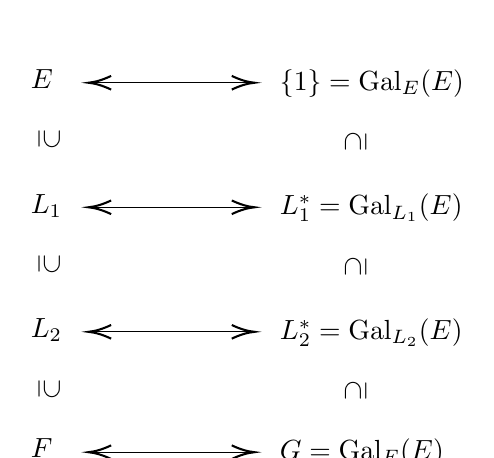
\begin{tikzpicture}[x=0.75pt,y=0.75pt,yscale=-1,xscale=1]
%uncomment if require: \path (0,334); %set diagram left start at 0, and has height of 334

%Straight Lines [id:da9812720467145646] 
\draw    (252,110) -- (328,110) ;
\draw [shift={(330,110)}, rotate = 180] [color={rgb, 255:red, 0; green, 0; blue, 0 }  ][line width=0.75]    (10.93,-3.29) .. controls (6.95,-1.4) and (3.31,-0.3) .. (0,0) .. controls (3.31,0.3) and (6.95,1.4) .. (10.93,3.29)   ;
\draw [shift={(250,110)}, rotate = 0] [color={rgb, 255:red, 0; green, 0; blue, 0 }  ][line width=0.75]    (10.93,-3.29) .. controls (6.95,-1.4) and (3.31,-0.3) .. (0,0) .. controls (3.31,0.3) and (6.95,1.4) .. (10.93,3.29)   ;
%Straight Lines [id:da02579375733408673] 
\draw    (252,170) -- (328,170) ;
\draw [shift={(330,170)}, rotate = 180] [color={rgb, 255:red, 0; green, 0; blue, 0 }  ][line width=0.75]    (10.93,-3.29) .. controls (6.95,-1.4) and (3.31,-0.3) .. (0,0) .. controls (3.31,0.3) and (6.95,1.4) .. (10.93,3.29)   ;
\draw [shift={(250,170)}, rotate = 0] [color={rgb, 255:red, 0; green, 0; blue, 0 }  ][line width=0.75]    (10.93,-3.29) .. controls (6.95,-1.4) and (3.31,-0.3) .. (0,0) .. controls (3.31,0.3) and (6.95,1.4) .. (10.93,3.29)   ;
%Straight Lines [id:da07950394444647135] 
\draw    (252,230) -- (328,230) ;
\draw [shift={(330,230)}, rotate = 180] [color={rgb, 255:red, 0; green, 0; blue, 0 }  ][line width=0.75]    (10.93,-3.29) .. controls (6.95,-1.4) and (3.31,-0.3) .. (0,0) .. controls (3.31,0.3) and (6.95,1.4) .. (10.93,3.29)   ;
\draw [shift={(250,230)}, rotate = 0] [color={rgb, 255:red, 0; green, 0; blue, 0 }  ][line width=0.75]    (10.93,-3.29) .. controls (6.95,-1.4) and (3.31,-0.3) .. (0,0) .. controls (3.31,0.3) and (6.95,1.4) .. (10.93,3.29)   ;
%Straight Lines [id:da23871652949443423] 
\draw    (252,288) -- (328,288) ;
\draw [shift={(330,288)}, rotate = 180] [color={rgb, 255:red, 0; green, 0; blue, 0 }  ][line width=0.75]    (10.93,-3.29) .. controls (6.95,-1.4) and (3.31,-0.3) .. (0,0) .. controls (3.31,0.3) and (6.95,1.4) .. (10.93,3.29)   ;
\draw [shift={(250,288)}, rotate = 0] [color={rgb, 255:red, 0; green, 0; blue, 0 }  ][line width=0.75]    (10.93,-3.29) .. controls (6.95,-1.4) and (3.31,-0.3) .. (0,0) .. controls (3.31,0.3) and (6.95,1.4) .. (10.93,3.29)   ;

% Text Node
\draw (221,102.4) node [anchor=north west][inner sep=0.75pt]    {$E$};
% Text Node
\draw (341,102.4) node [anchor=north west][inner sep=0.75pt]    {$\{1\} =\Gal_{E}( E)$};
% Text Node
\draw (237.6,131) node [anchor=north west][inner sep=0.75pt]  [rotate=-90]  {$\supseteq $};
% Text Node
\draw (372.4,145) node [anchor=north west][inner sep=0.75pt]  [rotate=-270]  {$\supseteq $};
% Text Node
\draw (221,162.4) node [anchor=north west][inner sep=0.75pt]    {$L_{1}$};
% Text Node
\draw (341,162.4) node [anchor=north west][inner sep=0.75pt]    {$L^{*}_{1} =\Gal_{L_{1}}( E)$};
% Text Node
\draw (221,222.4) node [anchor=north west][inner sep=0.75pt]    {$L_{2}$};
% Text Node
\draw (341,222.4) node [anchor=north west][inner sep=0.75pt]    {$L^{*}_{2} =\Gal_{L_{2}}( E)$};
% Text Node
\draw (237.6,191) node [anchor=north west][inner sep=0.75pt]  [rotate=-90]  {$\supseteq $};
% Text Node
\draw (372.4,205) node [anchor=north west][inner sep=0.75pt]  [rotate=-270]  {$\supseteq $};
% Text Node
\draw (237.6,251) node [anchor=north west][inner sep=0.75pt]  [rotate=-90]  {$\supseteq $};
% Text Node
\draw (372.4,265) node [anchor=north west][inner sep=0.75pt]  [rotate=-270]  {$\supseteq $};
% Text Node
\draw (221,280.4) node [anchor=north west][inner sep=0.75pt]    {$F$};
% Text Node
\draw (341,280.4) node [anchor=north west][inner sep=0.75pt]    {$G=\Gal_{F}( E)$};
\end{tikzpicture}
\end{center}
\end{thm}
\begin{pf}
Let $L \in \Int(E/F)$ and $H \in \Sub(G)$. Recall Theorem 7.12, which states that if 
$G = \Gal_{F_1}(E_1)$, then $E_1^{G_1} = F_1$. Therefore, we have 
\[ (L^*)^* = (\Gal_L(E))^* = E^{\Gal_L(E)} = L. \] 
Moreover, Theorem 9.6 states that if $G_1 \subseteq \Aut(E_1)$, then $\Gal_{E_1^{G_1}}(E_1) = G_1$, 
so it follows that 
\[ (H^*)^* = (E^H)^* = \Gal_{E^H}(E) = H. \]
In particular, we see that the maps $L \mapsto L^*$ and $H \mapsto H^*$ are inverses of each other. 

Now, let $L_1, L_2 \in \Int(E/F)$. Since $E/F$ is the splitting field of some separable polynomial 
$f(x) \in F[x]$, we have that $E/L_1$ and $E/L_2$ are also Galois extensions as $E$ is the 
splitting field of $f(x)$ over $L_1$ and $L_2$ respectively. If $L_2 \subseteq L_1$, then 
\[ L_1^* = \Gal_{L_1}(E) \subseteq \Gal_{L_2}(E) = L_2^*. \]
Moreover, we have 
\[ [L_1 : L_2] = \frac{[E : L_2]}{[E : L_1]} = 
\frac{\lvert\Gal_{L_2}(E)\rvert}{\lvert\Gal_{L_1}(E)\rvert} = \frac{|L_2^*|}{|L_1^*|} = 
[L_2^* : L_1^*]. \]
Similarly, for $H_1, H_2 \in \Sub(G)$, we see that if $H_2 \subseteq H_1$, then 
\[ H_1^* = E^{H_1} \subseteq E^{H_2} = H_2^*, \]
and we have 
\[ [H_1 : H_2] = \frac{|H_1|}{|H_2|} 
= \frac{\lvert\Gal_{E^{H_1}}(E)\rvert}{\lvert\Gal_{E^{H_2}}(E)\rvert} 
= \frac{[E : E^{H_1}]}{[E : E^{H_2}]} = 
[E^{H_2} : E^{H_1}] = [H_2^* : H_1^*]. \qedhere \]
\end{pf}

\begin{remark}
In the beginning of the course, we discussed the intermediate fields between $\Q$ and 
$E = \Q(\sqrt2, \sqrt3)$. At the time, it was not clear how many intermediate fields 
were between these two fields. We now know that $E/\Q$ is a Galois extension and that 
$\Gal_{\Q}(E)$ is a finite group. Since there are only finitely many subgroups of the 
finite group $\Gal_{\Q}(E)$, the Galois correspondence gives us the definitive answer that 
there are only finitely many intermediate fields between $\Q$ and $E$. Transforming 
a difficult question of infinite fields into an easier question of finite groups is 
the spirit of Galois theory. 
\end{remark}

We have previously seen that if $E/F$ is a finite Galois extension and $L \in \Int(E/F)$, then 
$L/F$ is not necessarily a Galois extension. For instance, by taking 
$E = \Q(\sqrt[3]{2}, \zeta_3)$, $L = \Q(\sqrt[3]{2})$, and $F = \Q$, we can see that $L/F$ 
is not Galois. 

\begin{center}
\tikzset{every picture/.style={line width=0.75pt}} %set default line width to 0.75pt        

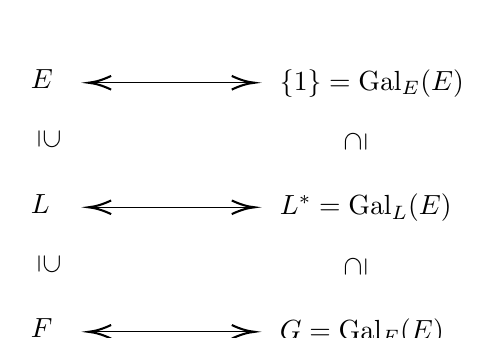
\begin{tikzpicture}[x=0.75pt,y=0.75pt,yscale=-1,xscale=1]
%uncomment if require: \path (0,334); %set diagram left start at 0, and has height of 334

%Straight Lines [id:da9812720467145646] 
\draw    (252,110) -- (328,110) ;
\draw [shift={(330,110)}, rotate = 180] [color={rgb, 255:red, 0; green, 0; blue, 0 }  ][line width=0.75]    (10.93,-3.29) .. controls (6.95,-1.4) and (3.31,-0.3) .. (0,0) .. controls (3.31,0.3) and (6.95,1.4) .. (10.93,3.29)   ;
\draw [shift={(250,110)}, rotate = 0] [color={rgb, 255:red, 0; green, 0; blue, 0 }  ][line width=0.75]    (10.93,-3.29) .. controls (6.95,-1.4) and (3.31,-0.3) .. (0,0) .. controls (3.31,0.3) and (6.95,1.4) .. (10.93,3.29)   ;
%Straight Lines [id:da02579375733408673] 
\draw    (252,170) -- (328,170) ;
\draw [shift={(330,170)}, rotate = 180] [color={rgb, 255:red, 0; green, 0; blue, 0 }  ][line width=0.75]    (10.93,-3.29) .. controls (6.95,-1.4) and (3.31,-0.3) .. (0,0) .. controls (3.31,0.3) and (6.95,1.4) .. (10.93,3.29)   ;
\draw [shift={(250,170)}, rotate = 0] [color={rgb, 255:red, 0; green, 0; blue, 0 }  ][line width=0.75]    (10.93,-3.29) .. controls (6.95,-1.4) and (3.31,-0.3) .. (0,0) .. controls (3.31,0.3) and (6.95,1.4) .. (10.93,3.29)   ;
%Straight Lines [id:da23871652949443423] 
\draw    (252,230) -- (328,230) ;
\draw [shift={(330,230)}, rotate = 180] [color={rgb, 255:red, 0; green, 0; blue, 0 }  ][line width=0.75]    (10.93,-3.29) .. controls (6.95,-1.4) and (3.31,-0.3) .. (0,0) .. controls (3.31,0.3) and (6.95,1.4) .. (10.93,3.29)   ;
\draw [shift={(250,230)}, rotate = 0] [color={rgb, 255:red, 0; green, 0; blue, 0 }  ][line width=0.75]    (10.93,-3.29) .. controls (6.95,-1.4) and (3.31,-0.3) .. (0,0) .. controls (3.31,0.3) and (6.95,1.4) .. (10.93,3.29)   ;

% Text Node
\draw (221,102.4) node [anchor=north west][inner sep=0.75pt]    {$E$};
% Text Node
\draw (341,102.4) node [anchor=north west][inner sep=0.75pt]    {$\{1\} =\Gal_{E}( E)$};
% Text Node
\draw (237.6,131) node [anchor=north west][inner sep=0.75pt]  [rotate=-90]  {$\supseteq $};
% Text Node
\draw (372.4,145) node [anchor=north west][inner sep=0.75pt]  [rotate=-270]  {$\supseteq $};
% Text Node
\draw (221,162.4) node [anchor=north west][inner sep=0.75pt]    {$L$};
% Text Node
\draw (341,162.4) node [anchor=north west][inner sep=0.75pt]    {$L^{*} =\Gal_{L}( E)$};
% Text Node
\draw (237.6,191) node [anchor=north west][inner sep=0.75pt]  [rotate=-90]  {$\supseteq $};
% Text Node
\draw (372.4,205) node [anchor=north west][inner sep=0.75pt]  [rotate=-270]  {$\supseteq $};
% Text Node
\draw (221,222.4) node [anchor=north west][inner sep=0.75pt]    {$F$};
% Text Node
\draw (341,222.4) node [anchor=north west][inner sep=0.75pt]    {$G=\Gal_{F}( E)$};
\end{tikzpicture}
\end{center}

The above diagram shows that if $L/F$ is Galois, then it corresponds to the group 
$G/L^*$, which is only well-defined if $L^*$ is a normal subgroup of $G$. The next 
two results are concerned with the normality of $L^*$. 

\begin{prop}
Let $E/F$ be a finite Galois extension with $G = \Gal_F(E)$. Let $L$ be an intermediate 
field of $E/F$. For any $\psi \in G$, we have 
\[ \Gal_{\psi(L)}(E) = \psi \Gal_L(E) \psi^{-1}. \]
\end{prop}
\begin{pf}
For any $\alpha \in \psi(L)$, we have $\psi^{-1}(\alpha) \in L$. Let $\phi \in \Gal_L(E)$. 
Then we obtain 
\[ \phi\psi^{-1}(\alpha) = \psi^{-1}(\alpha), \]
and hence 
\[ \psi\phi\psi^{-1}(\alpha) = \alpha. \]
It follows that $\psi\phi\psi^{-1} \in \Gal_{\psi(L)}(E)$ for all $\phi \in \Gal_L(E)$, 
so $\psi\Gal_L(E)\psi^{-1} \subseteq \Gal_{\psi(L)}(E)$. On the other hand, we have 
\[ |\psi\Gal_L(E)\psi^{-1}| = \lvert \Gal_L(E) \rvert 
= [E : L] = [E : \psi(L)] = \lvert \Gal_{\psi(L)}(E)|, \]
where the third equality is obtained by considering the basis of $E$ over $L$. Thus, we conclude that 
\[ \Gal_{\psi(L)}(E) = \psi \Gal_L(E) \psi^{-1}. \qedhere \]
\end{pf}

The following theorem gives a criterion for $L/F$ to be a Galois extension. 

\begin{thm}
Define $E/F$, $L$, and $L^*$ as in Theorem 9.10 (the Galois correspondence). Then 
$L/F$ is a Galois extension if and only if $L^*$ is a normal subgroup of $G$. 
In this case, we have 
\[ \Gal_F(L) \cong G/L^*. \]
\end{thm}
\begin{pf}
Note that 
\begin{align*}
    L/F \text{ is Galois} &\iff 
    \psi(L) = L \text{ for all } \psi \in \Gal_F(E) \\
    &\iff \Gal_{\psi(L)}(E) = \Gal_L(E) \text{ for all } \psi \in \Gal_F(E) \\
    &\iff \psi \Gal_L(E) \psi^{-1} = \Gal_L(E) \text{ for all } \psi \in \Gal_F(E) \text { (by Proposition 9.11)} \\
    &\iff L^* = \Gal_L(E) \text{ is a normal subgroup of $G$.}
\end{align*}
Now, if $L/F$ is a Galois extension, then the restriction map 
\[ G = \Gal_F(E) \to \Gal_F(L) : \psi \mapsto \psi|_L \]
is well-defined. Moreover, it is surjective and has kernel $\Gal_L(E) = L^*$. 
Therefore, we have 
\[ \Gal_F(L) \cong G/L^*. \qedhere \]
\end{pf}

\begin{exmp}
Let $p$ be a prime and let $q = p^n$. Consider the finite field $\F_q$, which is an extension of 
$\F_p$ of degree $n$. We saw in Assignment 4 that the {\bf Frobenius automorphism} of $\F_q$ is 
defined by 
\[ \sigma_p : \F_q \to \F_q : \alpha \mapsto \alpha^p. \]
For all $\alpha \in \F_q$, we have 
\[ \sigma_p^n(\alpha) = \alpha^{p^n} = \alpha, \]
so $\sigma_p^n = 1$. If $1 \leq m < n$, then $\sigma_p^m(\alpha) = \alpha^{p^m}$. 
Since the polynomial $x^{p^m} - x$ has at most $p^m$ roots in $\F_q$, there exists 
$\alpha \in \F_q$ such that $\alpha^{p^m} - \alpha \neq 0$, and hence $\sigma_p^m \neq 1$. 
Thus, $\sigma_p$ has order $n$. Now, let $G = \Gal_{\F_p}(\F_q)$. It follows that 
\[ n = |\langle \sigma_p \rangle| \leq |G| = [\F_q : \F_p] = n, \]
so $G = \langle \sigma_p \rangle$ is a cyclic group of order $n$. 

Consider a subgroup $H$ of $G$ of order $d$. Then $d \mid n$ and $[G : H] = n/d$. 
By the Galois correspondence, we have 
\[ n/d = [G : H] = [H^* : G^*] = [\F_q^H : \F_q^G] = [\F_q^H : \F_q]. \]
Thus, we see that $H^* = \F_q^H = \F_{p^{n/d}}$. We illustrate this in the following diagram. 

\begin{center}
    

\tikzset{every picture/.style={line width=0.75pt}} %set default line width to 0.75pt        

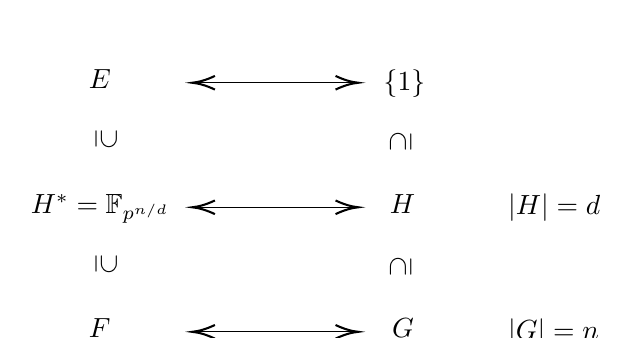
\begin{tikzpicture}[x=0.75pt,y=0.75pt,yscale=-1,xscale=1]
%uncomment if require: \path (0,334); %set diagram left start at 0, and has height of 334

%Straight Lines [id:da9812720467145646] 
\draw    (272,110) -- (348,110) ;
\draw [shift={(350,110)}, rotate = 180] [color={rgb, 255:red, 0; green, 0; blue, 0 }  ][line width=0.75]    (10.93,-3.29) .. controls (6.95,-1.4) and (3.31,-0.3) .. (0,0) .. controls (3.31,0.3) and (6.95,1.4) .. (10.93,3.29)   ;
\draw [shift={(270,110)}, rotate = 0] [color={rgb, 255:red, 0; green, 0; blue, 0 }  ][line width=0.75]    (10.93,-3.29) .. controls (6.95,-1.4) and (3.31,-0.3) .. (0,0) .. controls (3.31,0.3) and (6.95,1.4) .. (10.93,3.29)   ;
%Straight Lines [id:da02579375733408673] 
\draw    (272,170) -- (348,170) ;
\draw [shift={(350,170)}, rotate = 180] [color={rgb, 255:red, 0; green, 0; blue, 0 }  ][line width=0.75]    (10.93,-3.29) .. controls (6.95,-1.4) and (3.31,-0.3) .. (0,0) .. controls (3.31,0.3) and (6.95,1.4) .. (10.93,3.29)   ;
\draw [shift={(270,170)}, rotate = 0] [color={rgb, 255:red, 0; green, 0; blue, 0 }  ][line width=0.75]    (10.93,-3.29) .. controls (6.95,-1.4) and (3.31,-0.3) .. (0,0) .. controls (3.31,0.3) and (6.95,1.4) .. (10.93,3.29)   ;
%Straight Lines [id:da23871652949443423] 
\draw    (272,230) -- (348,230) ;
\draw [shift={(350,230)}, rotate = 180] [color={rgb, 255:red, 0; green, 0; blue, 0 }  ][line width=0.75]    (10.93,-3.29) .. controls (6.95,-1.4) and (3.31,-0.3) .. (0,0) .. controls (3.31,0.3) and (6.95,1.4) .. (10.93,3.29)   ;
\draw [shift={(270,230)}, rotate = 0] [color={rgb, 255:red, 0; green, 0; blue, 0 }  ][line width=0.75]    (10.93,-3.29) .. controls (6.95,-1.4) and (3.31,-0.3) .. (0,0) .. controls (3.31,0.3) and (6.95,1.4) .. (10.93,3.29)   ;

% Text Node
\draw (219,102.4) node [anchor=north west][inner sep=0.75pt]    {$E$};
% Text Node
\draw (361,102.4) node [anchor=north west][inner sep=0.75pt]    {$\{1\}$};
% Text Node
\draw (235,131) node [anchor=north west][inner sep=0.75pt]  [rotate=-90]  {$\supseteq $};
% Text Node
\draw (364,145) node [anchor=north west][inner sep=0.75pt]  [rotate=-270]  {$\supseteq $};
% Text Node
\draw (191,162.4) node [anchor=north west][inner sep=0.75pt]    {$H^{*}  = \F_{p^{n/d}}$};
% Text Node
\draw (364,162.4) node [anchor=north west][inner sep=0.75pt]    {$H$};
% Text Node
\draw (235,191) node [anchor=north west][inner sep=0.75pt]  [rotate=-90]  {$\supseteq $};
% Text Node
\draw (364,205) node [anchor=north west][inner sep=0.75pt]  [rotate=-270]  {$\supseteq $};
% Text Node
\draw (219,222.4) node [anchor=north west][inner sep=0.75pt]    {$F$};
% Text Node
\draw (365,222.4) node [anchor=north west][inner sep=0.75pt]    {$G$};
% Text Node
\draw (421,162.4) node [anchor=north west][inner sep=0.75pt]    {$|H| = d$};
% Text Node
\draw (421,222.4) node [anchor=north west][inner sep=0.75pt]    {$|G| = n$};

\end{tikzpicture}
\end{center}
\end{exmp}

\begin{exmp}
Let $E$ be the splitting field of $x^5 - 7$ over $\Q$ in $\C$. Then $E = \Q(\alpha, \zeta_5)$ 
with $\alpha = \sqrt[5]{7}$ and $\zeta_5 = e^{2\pi i/5}$. The minimal polynomials of $\alpha$ and 
$\zeta_5$ are $x^5 - 7$ and $x^4 + x^3 + x^2 + x + 1$ respectively. 

\begin{center} \includegraphics[width=0.35\textwidth]{9-14-1.png} \end{center}

Since $[\Q(\alpha) : \Q] = 5$ and $[\Q(\zeta_5) : \Q] = 4$ are both divisors of 
$[E : \Q]$, it follows that $[E : \Q]$ is divisible by $20$. Hence, we have 
$[E : \Q(\zeta_5)] \geq 5$. Moreover, note that $E = \Q(\alpha, \zeta_5) = 
\Q(\zeta_5)(\alpha)$ and the minimal polynomial of $\alpha$ over $\Q(\zeta_5)$ must 
divide $x^5 - 7$. Hence, we get $[E : \Q(\zeta_5)] \leq 5$. Finally, we obtain 
\[ [E : \Q] = [E : \Q(\zeta_5)] \cdot [\Q(\zeta_5) : \Q] = 5 \cdot 4 = 20. \]
Thus, $G = \Gal_\Q(F)$ is a group (in particular, a subgroup of $S_5$) of order $20$. 

Now, for each $\psi \in G$, its action is determined by $\psi(\alpha)$ and $\psi(\zeta_5)$. 
We write $\psi = \psi_{k,s}$ if $\psi(\alpha) = \alpha\zeta_5^k$ where $k \in \Z_5$ and 
$\psi(\zeta_5) = \zeta_5^s$ where $s \in \Z_5^*$. Define 
\begin{align*}
    \sigma = \psi_{1,1} &= \begin{cases} \alpha \mapsto \alpha\zeta_5 \\ \zeta_5 \mapsto \zeta_5, 
    \end{cases} \\
    \tau = \psi_{0,2} &= \begin{cases} \alpha \mapsto \alpha \\ \zeta_5 \mapsto \zeta_5^2. \end{cases}
\end{align*}
It can be verified that $\tau\sigma = \sigma^2\tau$, and we have 
\[ G = \langle \sigma, \tau : \sigma^5 = \tau^4 = 1,\, \tau\sigma = \sigma^2\tau \rangle. \]
It follows that 
\[ G = \{\sigma^a \tau^b : a \in \{0, 1, 2, 3, 4\},\, b \in \{0, 1, 2, 3\}\}. \]
Since $|G| = 20$, Lagrange's theorem implies that the possible subgroups of $G$ 
are of order $1$, $2$, $4$, $5$, $10$, and $20$. We now look at the subgroups of $G$. 

Note that $|G| = 20 = 4 \cdot 5$, so let $n_p$ be the number of Sylow $p$-subgroups of $G$. 
By the third Sylow theorem, we have $n_2 \mid 5$ and $n_2 \equiv 1 \pmod 2$, so $n_2 \in \{1, 5\}$. 
Moreover, we have $n_5 \mid 4$ and $n_5 \equiv 1 \pmod 5$, so $n_5 = 1$. Then 
$G$ has a unique Sylow $5$-subgroup, say $P_5$, which is of order $5$. Since 
$\langle \sigma \rangle$ is a subgroup of $G$ of order $5$, we have 
$P_5 = \langle \sigma \rangle \cong \Z/\langle 5 \rangle$. Note that the second Sylow theorem 
tells us that $P_5 \norm G$. Suppose to the contrary that $n_2 = 1$. Then there is a unique 
Sylow $2$-subgroup of $G$, say $P_4 = \langle \tau \rangle \cong \Z/\langle 4 \rangle$, 
in which case we have $P_4 \norm G$. Since $|P_4 \cap P_5| = 1$, it follows that 
\[ G \cong P_4 \times P_5 \cong \Z/\langle 4 \rangle \times \Z/\langle 5 \rangle \cong 
\Z/\langle 20 \rangle. \]
This is a contradiction as $G$ is not abelian. Thus, there must be $5$ Sylow $2$-subgroups of $G$. 

We have seen that $\tau \in G$ is of order $4$. Hence, the cyclic group $\langle \tau \rangle$ 
is a Sylow $2$-subgroup of $G$ and all other Sylow $2$-subgroups of $G$ are conjugate to it. 
Since the elements of $G$ are all of the form $\sigma^a \tau^b$, we have 
\[ \sigma^a\tau^b(\tau)\tau^{-b}\sigma^{-a} = \sigma^a \tau \sigma^{-a} \]
where $a \in \{0, 1, 2, 3, 4\}$. Using the relation $\tau\sigma = \sigma^2\tau$, we obtain 
\[ \langle \sigma^4 \tau \sigma^{-4} \rangle = \langle \sigma^{-1}\tau\sigma \rangle 
= \langle \sigma\tau \rangle = \langle \psi_{1,2} \rangle. \]
By the same argument, the Sylow $2$-subgroups of $G$ are 
\[ \langle \psi_{0,2} \rangle, \langle \psi_{1,2} \rangle, \langle \psi_{2,2} \rangle, \langle \psi_{3,2} \rangle, \langle \psi_{4,2} \rangle. \]
Moreover, since each subgroup of $G$ of order $2$ is contained in a Sylow $2$-group, we see that 
\[ \langle \psi_{0,2}^2 \rangle, \langle \psi_{1,2}^2 \rangle, \langle \psi_{2,2}^2 \rangle, \langle \psi_{3,2}^2 \rangle, \langle \psi_{4,2}^2 \rangle \]
are all subgroups of $G$ of order $2$. Finally, for a subgroup $H$ of $G$ of order $10$, 
since $P_5$ is the only subgroup of order $5$, we have $H \supseteq P_5 = \langle \sigma \rangle$. 
Therefore, $\sigma^a \tau^b \in H$ if and only if $\tau^b \in H$. The only element 
of the form $\tau^b$ of order $2$ is $\tau^2$, so $H = \langle \sigma, \tau^2 \rangle$. 
We summarize our results with the following diagram. 

\begin{center} \includegraphics[width=0.85\textwidth]{9-14-2.png} \end{center}

For an intermediate field $L$ of $E/\Q$, consider $L^* = \Gal_L(E)$. For instance, for the 
intermediate field $\Q(\zeta_5)$, note that $\psi_{1,1}(\zeta_5) = \zeta_5$, so 
$\Q(\zeta_5)^* \supseteq \langle \psi_{1,1} \rangle$. Since $|\langle \psi_{1,1} \rangle| 
= [\langle \psi_{1,1} \rangle : \{1\}] = 5$ and 
\[ 5 = [E : \Q(\zeta_5)] = [\Q(\zeta_5)^* : \{1\}], \]
we have $\Q(\zeta_5)^* = \langle \psi_{1,1} \rangle$. Also, notice that 
\[ \psi_{1,2}(\alpha\zeta_5^r) = \alpha\zeta_5 \zeta_5^{2r} = \alpha \zeta_5^{2r+1}. \]
If $\psi_{1,2}$ fixes $\alpha\zeta_5^r$, then $r \equiv 2r + 1 \pmod 5$, so we must have 
$r \equiv 4 \pmod 5$. Hence, we have $\Q(\alpha\zeta_5^4)^* \supseteq \langle \psi_{1,2} \rangle$.
Since $|\langle \psi_{1,2} \rangle| = [\langle \psi_{1,2} \rangle : \{1\}] = 4$ and 
$[E : \Q(\alpha\zeta_5^4)] = 4$, we get $\Q(\alpha\zeta_5^4)^* = \langle \psi_{1,2} \rangle$. 
A similar argument gives us $\langle \psi_{r,2} \rangle$ for all $r \in \{0, 1, 2, 3, 4\}$. 

Consider $\beta = \zeta_5 + \zeta_5^{-1} \in \R$. We have 
\begin{align*}
    \beta^2 + \beta - 1 
    &= (\zeta_5 + \zeta_5^{-1})^2 + (\zeta_5 + \zeta_5^{-1}) - 1 \\
    &= \zeta_5^2 + 2 + \zeta_5^{-2} + \zeta_5 + \zeta_5^{-1} - 1 \\
    &= 1 + \zeta_5 + \zeta_5^2 + \zeta_5^3 + \zeta_5^4 
    = 0.
\end{align*}
Since $x^2 + x - 1 = 0$ has no roots in $\Q$, we have 
\[ [\Q(\beta) : \Q] = 2. \]
In a similar way, one can obtain $[\Q(\alpha, \beta) : \Q(\alpha)] = 2$. We now have the following 
correspondence diagram of the intermediate fields of $E/\Q$. 

\begin{center} \includegraphics[width=\textwidth]{9-14-3.png} \end{center}
\end{exmp}

\newpage 
\section{Cyclic extensions}

Recall that if $E/F$ is a Galois extension, then we say that $E/F$ is cyclic if its Galois 
group $\Gal_F(E)$ is cyclic. 
We will now focus on cyclic extensions,
which will be used when we discuss solvability by radicals in the 
following section. 

\begin{lemma}[Dedekind's lemma]
Let $K$ and $L$ be fields. For each $1 \leq i \leq n$, let 
$\psi_i : L \to K$ be a distinct non-zero homomorphism. If $c_1, \dots, c_n \in K$ and 
\[ c_1\psi_1(\alpha) + \cdots + c_n\psi_n(\alpha) = 0 \]
for all $\alpha \in L$, then $c_1 = c_2 = \cdots = c_n = 0$. 
\end{lemma}
\begin{pf}
Suppose to the contrary that there exists $c_1, \dots, c_n \in K$, not all zero, such that 
\[ c_1\psi_1(\alpha) + \cdots + c_n\psi_n(\alpha) = 0 \]
for all $\alpha \in L$. Let $m \geq 2$ be the smallest positive integer such that 
\[ c_1\psi_1(\alpha) + \cdots + c_m\psi_m(\alpha) = 0 \tag{1} \]
for all $\alpha \in L$. Since $m$ is minimal, we have $c_i \neq 0$ for all $1 \leq i \leq m$. 
Note that $\psi_1 \neq \psi_2$ as the homomorphisms are distinct, so we can choose $\beta \in L$ 
such that $\psi_1(\beta) \neq \psi_2(\beta)$. By the injectivity of $\psi_1$, we can 
assume that $\psi_1(\beta) \neq 0$. By (1), we have 
\[ c_1\psi_1(\alpha\beta) + \cdots + c_m\psi_m(\alpha\beta) = 0 \]
for all $\alpha \in L$. Dividing this equation by $\psi_1(\beta)$ yields 
\[ c_1\psi_1(\alpha) + c_2 \psi_2(\alpha) \frac{\psi_2(\beta)}{\psi_1(\beta)} 
\cdots + c_m\psi_m(\alpha) \frac{\psi_m(\beta)}{\psi_1(\beta)} = 0 \tag{2} \]
for all $\alpha \in L$. Subtracting (2) from (1), we obtain 
\[ c_2 \left(1 - \frac{\psi_2(\beta)}{\psi_1(\beta)} \right) \psi_2(\alpha) 
+ \cdots + c_m \left( 1 - \frac{\psi_m(\beta)}{\psi_1(\beta)} \right) \psi_m(\alpha) = 0 \tag{3} \]
for all $\alpha \in L$. Note that 
\[ c_2 \left(1 - \frac{\psi_2(\beta)}{\psi_1(\beta)} \right) \neq 0, \]
so (3) contradicts the minimality of $m$. Thus, we must have $c_1 = c_2 = \cdots = c_n = 0$. 
\end{pf}

In Example 9.14, we saw that $E = \Q(\alpha, \zeta_5)$ is the splitting field of $x^5 - 7$ 
over $\Q$ where $\alpha = \sqrt[5]{7}$ and $\zeta_5 = e^{2\pi i/5}$. 
Recall that $E$ is a simple extension of $\Q(\zeta_5)$. Moreover, its Galois group is 
given by $\Gal_{\Q(\zeta_5)}(E) \cong \Z/\langle 5 \rangle$, which is cyclic. 
The following theorem is a generalization of this example. 

\begin{thm}
Let $F$ be a field and let $n \in \N$. Suppose that $\ch(F) = 0$ or $\ch(F) = p$ where 
$p \nmid n$. Moreover, assume that $x^n - 1$ splits over $F$. 
\begin{enumerate}[(1)]
    \item If the Galois extension $E/F$ is cyclic of degree $n$, then $E = F(\alpha)$ for some 
    $\alpha \in E$ with $\alpha^n \in F$. In particular, $x^n - \alpha^n$ is the minimal 
    polynomial of $\alpha$ over $F$. 
    \item If $E = F(\alpha)$ with $\alpha^n \in F$, then $E/F$ is a cyclic extension of degree $d$ 
    where $d \mid n$ and $\alpha^d \in F$. In particular, $x^d - \alpha^d$ is the minimal 
    polynomial of $\alpha$ over $F$. 
\end{enumerate}
\end{thm}
\begin{pf}
Let $\zeta_n \in F$ be a primitive $n$-th root of unity; that is, $\zeta_n^n = 1$ and 
$\zeta_n^k \neq 1$ for all $1 \leq k < n$. Note that $x^n - 1$ is separable since 
$\ch(F) = 0$ or $\ch(F) = p$ where $p \nmid n$. Hence, the elements 
$1, \zeta_n, \zeta_n^2, \dots, \zeta_n^{n-1}$ are all distinct. 
\begin{enumerate}[(1)]
    \item Let $G = \Gal_F(E)$ be cyclic with order $n$. In particular, we have 
    $G = \langle \psi \rangle \cong \Z/\langle n \rangle$ for some $\psi \in G$. 
    We apply Dedekind's lemma in the case where $K = L = E$, the homomorphisms $\psi_i$ are the 
    elements of $G$, and $c_i = \zeta_n^{-(i-1)}$ for all $1 \leq i \leq n$. Clearly, we have 
    $c_i \neq 0$ for all $1 \leq i \leq n$, so there exists $u \in E$ such that 
    \[ \alpha = u + \zeta_n^{-1} \psi(u) + \cdots + \zeta_n^{-(n-1)} \psi^{n-1}(u) \neq 0. \]
    Note that 
    \begin{align*}
        \id(\alpha) &= \alpha, \\
        \psi(\alpha) &= \alpha\zeta_n, \\
        \psi^2(\alpha) &= \alpha\zeta_n^2, \\
        &\;\;\vdots \\
        \psi^{n-1}(\alpha) &= \alpha\zeta_n^{n-1}. 
    \end{align*}
    Hence, we see that $\alpha, \alpha\zeta_n, \dots, \alpha\zeta_n^{n-1}$ are conjugates of each other; 
    that is, they have the same minimal polynomial over $F$, say $p(x)$. These elements 
    are also distinct, so it follows that $\deg(p) = n$. Moreover, since $p(x) \in F[x]$, we have 
    \[ p(0) = \pm\alpha(\alpha\zeta_n) \cdots (\alpha\zeta_n^{n-1}) = \pm\alpha^n \zeta_n^{n(n-1)/2} \in F. \]
    We know that $\zeta_n \in F$, so $\alpha^n \in F$ as well. Since $\alpha$ is a root of $x^n - \alpha^n
    \in F[x]$ and $\deg(p) = n$, we have $p(x) = x^n - \alpha^n$. Also, since $F(\alpha) \subseteq E$
    and 
    \[ [F(\alpha) : F] = \deg(p) = n = [E : F], \]
    it follows that $E = F(\alpha)$. 
    
    \item Suppose that $E = F(\alpha)$ with $\alpha^n \in F$. Let $p(x)$ be the minimal polynomial 
    of $\alpha$ over $F$. Since $\alpha$ is a root of $x^n - \alpha^n \in F[x]$, we have $p(x) 
    \mid x^n - \alpha^n$. Then, the roots of $p(x)$ are of the form $\alpha\zeta_n^i$ for some 
    $i$, so we have $p(0) = \pm\alpha^d \zeta_n^k$ where $d = \deg(p)$ is the number 
    of roots of $p(x)$ (as the roots are distinct) and $k \in \Z$. Now, 
    $p(0) \in F$ and $\zeta_n \in F$, so $\alpha^d \in F$ as well. Then $x^d - \alpha^d \in F[x]$ 
    has $\alpha$ as a root, so $p(x) \mid x^d - \alpha^d$. Since $\deg(p) = d$ and 
    $p(x)$ is monic, it follows that $p(x) = x^d - \alpha^d$. 
    
    We claim that $d \mid n$. Suppose otherwise, say $n = qd + r$ where $q \in \Z$ and $0 < r < d$. 
    Since $\alpha^d$ and $\alpha^n$ are in $F$, we have 
    \[ \alpha^r = \alpha^{n-qd} = (\alpha^n)(\alpha^{-d})^q \in F. \]
    Then $\alpha$ is a root of $x^r - \alpha^r \in F[x]$. It follows that 
    $p(x) \mid x^r - \alpha^r$, which is a contradiction as we have $\deg(p) = d > r$. 
    
    Now, since $d \mid n$, we have $n = md$ for some $m \in \Z$. We know that $p(x) = x^d - \alpha^d$,
    so the roots of $p(x)$ are given by 
    \[ \alpha, \alpha\zeta_n^m, \alpha\zeta_n^{2m}, \dots, \alpha\zeta_n^{(d-1)m}. \]
    Since $\zeta_n \in F$, it follows that $E = F(\alpha)$ is the splitting field of the 
    separable polynomial $p(x)$ over $F$, and hence is Galois. Choose 
    $\psi \in G = \Gal_F(E)$ such that $\psi(\alpha) = \alpha\zeta_n^m$. Then 
    $G = \langle \psi \rangle \cong \Z/\langle d \rangle$, so $E/F$ is a cyclic extension of degree $d$. 
    \qedhere 
\end{enumerate}
\end{pf}

When the degree of the polynomial and the characteristic of the field are both equal to 
a prime $p$, the criterion to be a cyclic extension is slightly more complicated. 

\begin{thm}
Let $F$ be a field with $\ch(F) = p$, where $p$ is a prime. 
\begin{enumerate}[(1)]
    \item If $x^p - x - a \in F[x]$ is irreducible, then its splitting field $E/F$ is a 
    cyclic extension of degree $p$. 
    \item If $E/F$ is a cyclic extension of degree $p$, then $E/F$ is the splitting field 
    of some irreducible polynomial of the form $x^p - x - a \in F[x]$. 
\end{enumerate}
\end{thm}
\begin{pf}~
\begin{enumerate}[(1)]
    \item Let $f(x) = x^p - x - a \in F[x]$ and let $\alpha$ be a root of $f(x)$. Since 
    $\ch(F) = p$, we have 
    \[ f(\alpha+1) = (\alpha+1)^p - (\alpha+1) - a = \alpha^p + 1 - \alpha - 1 - a = f(\alpha) = 0, \]
    so $\alpha+1$ is also a root of $f(x)$. Similarly, it can be shown that 
    $\alpha+2, \alpha+3, \dots, \alpha + (p-1)$ are roots of $p(x)$. Note that 
    $f(x)$ has at most $p$ distinct roots, so 
    \[ \alpha, \alpha+1, \alpha+2, \dots, \alpha + (p-1) \]
    are all the roots of $f(x)$. It follows that 
    $E = F(\alpha, \alpha+1, \dots, \alpha + (p-1)) = F(\alpha)$ and $[E : F] = \deg(f) = p$. 
    Since $\Z/\langle p \rangle$ is the only group of order $p$ (up to isomorphism), 
    we have $\Gal_F(E) \cong \Z/\langle p \rangle$. Indeed, observe that 
    $\Gal_F(E) = \langle \psi \rangle$, where $\psi : E \to E$ is the automorphism which fixes $F$ 
    and sends $\alpha$ to $\alpha+1$. 
    
    \item Suppose that $G = \Gal_F(E)$ be cyclic with order $p$, say $G = \langle \psi \rangle 
    \cong \Z/\langle p \rangle$. We apply Dedekind's lemma with $K = L = E$, 
    the homomorphisms being the elements of $G$, and $c_1 = c_2 = \cdots = c_p = 1$. 
    Since $c_i \neq 0$ for all $1 \leq i \leq p$, there exists $v \in E$ such that 
    \[ \beta := v + \psi(v) + \psi^2(v) + \cdots + \psi^{p-1}(v) \neq 0. \]
    Since $\psi^i(\beta) = \beta$ for all $0 \leq i \leq p-1$, we have $\beta \in F$. 
    Set $u = v/\beta$. Then we obtain 
    \begin{align*}
        u + \psi(u) + \psi^2(u) + \cdots + \psi^{p-1}(u)
        &= \frac v\beta + \psi\left(\frac v\beta\right) + \psi^2\left( \frac v\beta\right)
        + \cdots + \psi^{p-1}\left(\frac v\beta\right) \\
        &= \frac1\beta (v + \psi(v) + \psi^2(v) + \cdots + \psi^{p-1}(v)) \\
        &= \frac\beta\beta = 1.
    \end{align*}
    Now, define
    \[ \alpha := 0u - 1\psi(u) - 2\psi^2(u) - \cdots - (p-1)\psi^{p-1}(u). \]
    Then we have 
    \[ \psi(\alpha) = -\psi^2(u) - 2\psi^3(u) - \cdots - (p-1)\psi^p(u), \]
    so it follows that 
    \[ \psi(\alpha) - \alpha = \psi(u) + \psi^2(u) + \cdots + \psi^{p-1}(u) + \psi^p(u) = 1. \]
    In particular, we get $\psi(\alpha) = \alpha+1$. Since $\ch(F) = p$, we have 
    \[ \psi(\alpha^p) = \psi(\alpha)^p = (\alpha+1)^p = \alpha^p + 1, \]
    so we see that 
    \[ \psi(\alpha^p - \alpha) = \psi(\alpha^p) - \psi(\alpha) = (\alpha^p+1) - (\alpha+1) = \alpha^p 
    - \alpha. \]
    Hence, $\alpha^p - \alpha$ is fixed by $\psi$. Since $G = \langle \psi \rangle$, it follows that 
    $a = \alpha^p - \alpha \in F$ and $\alpha$ is a root of $x^p - x - a \in F[x]$. We have 
    $[E : F] = p$, so $[F(\alpha) : F]$ must be a factor of $p$. Since 
    $\alpha \notin F$ (as we showed that $\psi(\alpha) = \alpha+1$) and $p$ is prime, we have 
    $[F(\alpha) : F] = p$ and $E = F(\alpha)$. Finally, $[F(\alpha) : F] = p$ implies that 
    $x^p - x - a \in F[x]$ is the minimal polynomial of $\alpha$ over $F$. \qedhere 
\end{enumerate}
\end{pf}

\newpage 
\section{Solvability by radicals}

In this section, we will discuss radical extensions and solvability by radicals. Then, we will 
prove the Abel-Ruffini theorem, which states that a general polynomial of degree $\geq 5$ is 
not solvable by radicals. 

\subsection{Radical extensions}

\begin{defn}
A finite extension $E/F$ is said to be {\bf radical} if there exists a tower of fields 
\[ F = F_0 \subseteq F_1 \subseteq F_2 \subseteq \cdots \subseteq F_m = E \]
such that for all $1 \leq i \leq m$, we have $F_i = F_{i-1}(\alpha_i)$ 
with $\alpha_i^{d_i} \in F_{i-1}$ for some $d_i \in \N$. 
\end{defn}

\begin{lemma}
If $E/F$ is a finite separable radical extension, then its normal closure $N/F$ is also a radical 
extension.
\end{lemma}
\begin{pf}
Since $E/F$ is a finite separable extension, then by the primitive element theorem (Theorem 8.7), 
we have $E = F(\beta)$ for some $\beta \in E$. Since $E/F$ is also a radical extension, there 
exists a tower 
\[ F = F_0 \subseteq F_1 \subseteq F_2 \subseteq \cdots \subseteq F_m = E \]
such that for all $1 \leq i \leq m$, we have $F_i = F_{i-1}(\alpha_i)$ with 
$\alpha_i^{d_i} \in F_{i-1}$ for some $d_i \in \N$. Let $p(x) \in F[x]$ be the minimal polynomial 
of $\beta$ and let $\beta_1, \beta_2, \dots, \beta_m$ be the root of $p(x)$ with 
$\beta = \beta_1$. By the definition of normal closure and Theorem 8.10, we have 
$N = E(\beta_2, \dots, \beta_n) = F(\beta_1, \beta_2, \dots, \beta_n)$. Moreover, there is an 
$F$-isomorphism 
\[ \sigma_j : F(\beta) \to F(\beta_j) : \beta \mapsto \beta_j \]
for all $2 \leq j \leq n$. Since $N$ can be viewed as the splitting field of $p(x)$ over 
$F(\beta)$ and $F(\beta_j)$ respectively, then by Theorem 3.7, there exists 
$\psi_j : N \to N$ which extends $\sigma_j$ for all $2 \leq j \leq n$. Thus, we have 
$\psi_j \in \Gal_F(N)$ and $\psi_j(\beta) = \beta_j$. We obtain the tower of fields 
\begin{align*}
    F
    &\subseteq F_1 \subseteq F_2 \subseteq \cdots \subseteq F_m = E = F(\beta_1) = F(\beta_1)\psi_2(F_0) \\
    &\subseteq F(\beta_1)\psi_2(F_1) \subseteq F(\beta_2)\psi_2(F_2) \subseteq \cdots 
    \subseteq F(\beta_1)\psi_2(F_m) = F(\beta_1, \beta_2) = F(\beta_1, \beta_2)\psi_3(F_0) \\ 
    &\subseteq \cdots \\
    &\subseteq F(\beta_1, \beta_2, \dots, \beta_n) = N. 
\end{align*}
Since $F_i = F_{i-1}(\alpha_i)$ where $\alpha_i^{d_i} \in F_{i-1}$ for all $1 \leq i \leq m$, we have 
\begin{align*}
    F(\beta_1, \beta_2, \dots, \beta_{j-1}) \psi_j(F_i) 
    &= F(\beta_1, \beta_2, \dots, \beta_{j-1}) \psi_j(F_{i-1}(\alpha_i)) \\
    &= (F(\beta_1, \beta_2, \dots, \beta_{j-1}) \psi_j(F_{i-1})) (\psi_j(\alpha_i)) 
\end{align*}
and hence $(\psi_j(\alpha_i))^{d_i} = \psi_j(\alpha_i^{d_i}) \in \psi_j(F_{i-1})$. Thus, 
$N/F$ is a radical extension.
\end{pf}

\begin{remark}
As a consequence of Lemma 11.2, to consider a finite separable radical extension, it suffices to 
look at its normal closure, which is Galois. 
\end{remark}

\begin{defn}
Let $F$ be a field and let $f(x) \in F[x]$. We say that $f(x)$ is {\bf solvable by radicals} 
if there exists a radical extension $E/F$ such that $f(x)$ splits over $E$. 
\end{defn}

\begin{remark}
It is possible that $f(x) \in F[x]$ is solvable by radicals, but its splitting field is not a 
radical extension. On Assignment 11, we will show that $f(x) = x^3 - 3x + 1 \in \Q[x]$ is such 
an example. 
\end{remark}

\begin{remark}
Recall that an expression involving only $+, -, \times, \div, \sqrt[n]{}$ is called a radical. 
Let $F$ be a field and let $f(x) \in F[x]$ be separable. If $f(x)$ is solvable by radicals, 
then by the definition of a radical extension, all roots of $f(x)$ are radical. Conversely, if 
all roots of $f(x)$ are radical, then it is in some radical extension $E/F$. By Lemma 11.2, 
the normal closure $N/F$ of $E/F$ is radical; since $f(x)$ splits over $N$, we see that 
$f(x)$ is solvable by radicals. 
\end{remark}

\subsection{Radical solutions}

\begin{lemma}
Let $E/F$ be a field extension, and let $K$ and $L$ be intermediate fields of $E/F$. 
Suppose that $K/F$ is a finite Galois extension. Then the compositum $KL$ is a finite
Galois extension of $L$ and $\Gal_L(KL)$ is isomorphic to a subgroup of $\Gal_F(K)$. 
\end{lemma}
\begin{pf}
Since $K/F$ is a finite Galois extension, we have that $K$ is the splitting field of some 
$f(x) \in F[x]$ over $F$. Since $F \subseteq L$, we see that $KL$ is the splitting field of 
$f(x)$ over $L$ and hence is Galois. Consider the map 
\[ \Gamma : \Gal_L(KL) \to \Gal_F(K) : \psi \mapsto \psi|_K. \] 
Note that $\psi \in \Gal_L(KL)$ fixes $L$, so it also fixes $F$. Moreover, since $K$ is a Galois 
extension, we have $\psi(K) = K$. Thus, $\Gamma$ is a well-defined map. Furthermore, if 
$\psi|_K = 1_K$, then $\psi$ is trivial on $K$ and $L$, and hence trivial on $KL$. In particular, 
this shows that $\Gamma$ is injective. We conclude that $\Gal_L(KL) \cong \im\Gamma$, which is a subgroup 
of $\Gal_F(K)$. 
\end{pf}

\begin{defn}
Let $E/F$ be the splitting field of a separable polynomial $f(x) \in F[x]$. The {\bf Galois group 
of $f(x)$} is defined to be $\Gal_F(E)$ and is denoted by $\Gal(f)$. 
\end{defn}

\begin{thm}
Let $F$ be a field of characteristic $0$ and let $f(x) \in F[x] \setminus \{0\}$. Then 
$f(x)$ is solvable by radicals if and only if its Galois group is solvable. 
\end{thm}
\begin{pf}
Suppose that $f(x)$ is solvable by radicals; that is, $f(x)$ splits over some extension $E/F$ satisfying
\[ F = F_0 \subseteq F_1 \subseteq F_2 \subseteq \cdots \subseteq F_m = E \]
where for all $1 \leq i \leq m$, we have $F_i = F_{i-1}(\alpha_i)$ with $\alpha_i^{d_i} \in F_{i-1}$ 
for some $d_i \in \N$. Due to Lemma 11.2, we may assume without loss of generality that 
$E/F$ is Galois. Thus, $E/F$ is the splitting field of some separable polynomial $\hat f(x) \in F[x]$. 
Let 
\[ n = \prod_{i=1}^m d_i. \]
Let $L/E$ be the splitting field of $x^n-1$ over $E$ and let $\zeta_n \in L$ be a primitive 
$n$-th root of unity. Let $K = F(\zeta_n)$ and note that $L = E(\zeta_n) = KE$. For all 
$1 \leq i \leq m$, define 
\[ K_i = KF_i = F_i(\zeta_n). \] 
Then we have 
\[ F \subseteq F(\zeta_n) = K = K_0 \subseteq K_1 \subseteq \cdots \subseteq K_{m-1} \subseteq K_m 
= F_m(\zeta_n) = L. \]
Since $F_i = F_{i-1}(\alpha_i)$, we have $K_i = K_{i-1}(\alpha_i)$. Also, we have 
$\alpha_i^{d_i} \in F_{i-1} \subseteq K_{i-1}$ and $\zeta_n$ (and hence $\zeta_{d_i} = \zeta_n^{n/d_i}$)
is in $K_{i-1}$, so by Theorem 10.2, $K_i/K_{i-1}$ is a cyclic Galois extension. Note that $L$ 
is the splitting field of $\hat f(x)(x^n - 1)$ over $F$ (and also over $K_i$), so 
$L/F$ (and also $L/K_i$) is Galois. We have 
\[ G \supseteq \Gal_F(L) \supseteq \Gal_{K_0}(L) \supseteq \Gal_{K_1}(L) \supseteq 
\cdots \supseteq \Gal_{K_{m-1}}(L) \supseteq \Gal_{K_m}(L) = \{1\}. \]
Since $K_i/K_{i-1}$ is a Galois extension, then by Theorem 9.12, we obtain $\Gal_{K_i}(L) 
\norm \Gal_{K_{i-1}}(L)$ with 
\[ \Gal_{K_{i-1}}(L)/\Gal_{K_i}(L) \cong \Gal_{K_{i-1}}(K_i), \]
which is a cyclic group and hence abelian. Moreover, notice that 
\[ \Gal_F(L)/\Gal_{K_0}(L) = \Gal_F(L)/\Gal_K(L) \cong \Gal_F(K) = (\Z/\langle n \rangle)^* \]
is abelian, so $\Gal_F(L)$ is solvable. Let $\hat E$ be the splitting field of $f(x)$ over $F$, which 
is a subfield of $L$. Since $\hat E/F$ is a Galois extension, Theorem 9.12 gives 
\[ \Gal(f) = \Gal_F(\hat E) \cong \Gal_F(L)/\Gal_E(L). \]
Now, $\Gal(f)$ is a quotient group of the solvable group $\Gal_F(L)$, so by Theorem 6.6,
$\Gal(f)$ is solvable. 

\newpage 
Conversely, suppose that $G = \Gal(f)$ is solvable. Let $E/F$ be the splitting field of $f(x)$ 
and let $n = |G|$. Let $L/E$ be the splitting field of $x^n-1$ over $E$, and let 
$\zeta_n$ be a primitive $n$-th root of unity. Set $K = F(\zeta_n)$ and note that $L = E(\zeta_n) = 
KE$. Since $L = KE$ and $E/F$ is a finite Galois extension, Lemma 11.7 implies that $L/K$ is a 
finite Galois extension and $H = \Gal_K(L)$ is isomorphic to a subgroup of $G$. By Theorem 6.6, 
$H$ is solvable. Write 
\[ H = H_0 \supseteq H_1 \supseteq H_2 \supseteq \cdots \supseteq H_m = \{1\} \]
where $H_i \norm H_{i-1}$ and $H_{i-1}/H_i \cong C_{d_i}$ is a cyclic group of order $d_i$ 
for all $1 \leq i \leq m$. Since $H$ is a subgroup of $G$, we have $d_i \mid n$. Let 
$K_i = H_i^* = L^{H_i}$ for all $0 \leq i \leq m$. Then $\Gal_{K_i}(L) = H_i$, and we have a tower of 
fields 
\[ F \subseteq F(\zeta_n) = K = K_0 \subseteq K_1 \subseteq K_2 \subseteq \cdots \subseteq 
K_{m-1} \subseteq K_m = L = E(\zeta_n). \]
Since $H_i \norm H_{i-1}$, Theorem 9.12 implies that $K_i/K_{i-1}$ is Galois with 
\[ \Gal_{K_{i-1}}(K_i) \cong H_{i-1}/H_i \cong C_{d_i}. \]
Since $\zeta_n$ and hence $\zeta_{d_i} = \zeta_n^{n/d_i}$ is in $K_{i-1}$, then by Theorem 10.2, 
there exists $\alpha_i \in K_i$ such that $K_i = K_{i-1}(\alpha_i)$ and $\alpha_i^{d_i} 
\in K_{i-1}$. Moreover, we have $K_0 = K = F(\zeta_n)$ and $\zeta_n^n = 1 \in F$, so it follows that 
$L/F$ is a radical extension. Since all the roots of $f(x)$ are in $E$ and hence in $L$, 
we conclude that $f(x)$ is solvable by radicals. 
\end{pf}

\begin{prop}
Let $f(x) \in \Q[x]$ be an irreducible polynomial of prime degree $p$. If $f(x)$ has 
precisely two non-real roots in $\C$, then $\Gal(f) \cong S_p$. 
\end{prop}
\begin{pf}
Recall that the symmetric group $S_n$ can be generated by the cycles $(1\,2)$ and 
$(1\,2\,\cdots\,n)$. Thus, to show that $\Gal(f) \cong S_p$, it suffices to find 
an element of order $p$ and an element of order $2$ in $\Gal(f)$. Indeed, since 
$\deg(f) = p$, we see that $\Gal(f)$ is a subgroup of $S_p$ by Theorem 7.8. Let 
$\alpha$ be a root of $f(x)$. Since $f(x)$ is irreducible and of degree $p$, we have 
$[\Q(\alpha) : \Q] = p$. Hence, $p \mid \lvert\Gal(f)\rvert$. By Cauchy's theorem, 
there exists an element of order $p$ in $\Gal(f)$. Moreover, the complex conjugate map 
interchanges two non-real roots of $f(x)$ and fixes all the real roots, so it is 
an element of $\Gal(f)$ of order $2$. 
\end{pf}

\begin{exmp}
Consider the polynomial $f(x) = x^5 + 2x^3 - 24x - 2 \in \Q[x]$, which is irreducible by 
Eisenstein's criterion with $p = 2$. Since $f(-1) = 19$, $f(1) = -23$, 
$\lim_{x\to\infty} f(x) = \infty$, and $\lim_{x\to-\infty} f(x) = -\infty$, we see that 
$f(x)$ has at least three real roots. Let $\alpha_1, \alpha_2, \alpha_3, \alpha_4, \alpha_5$
be the roots of $f(x)$; that is, 
\[ f(x) = (x-\alpha_1)(x-\alpha_2)(x-\alpha_3)(x-\alpha_4)(x-\alpha_5). \]
Comparing the coefficients of the $x^4$ and $x^3$ terms, we get 
$\sum_{i=1}^5 \alpha_i = 0$ and $\sum_{i<j} \alpha_i \alpha_j = 2$. From the first sum, we have
\[ \left( \sum_{i=1}^5 \alpha_i \right)^2 = \sum_{i=1}^5 \alpha_i^2 + 2 \sum_{i<j} \alpha_i\alpha_j = 0. \]
Then, substituting the second sum into the above equation, we obtain 
\[ \sum_{i=1}^5 \alpha_i^2 = -4. \]
Thus, not all roots of $f(x)$ are real, so $f(x)$ has three real roots and two non-real roots. 
By Proposition 11.10, we have that $\Gal(f) \cong S_5$. But $S_5$ is not solvable, so by 
Theorem 11.9, the polynomial $f(x) = x^5 + 2x^3 - 24x - 2$ over $\Q$ is not solvable by radicals. 
\end{exmp}

\begin{thm}[Abel-Ruffini]
A general polynomial of degree $\geq 5$ is not solvable by radicals.
\end{thm}
\begin{pf}
From Example 11.11, we see that a general polynomial of degree $5$ is not solvable by radicals. 
The result follows by noting that $S_5 \subseteq S_n$ for all $n \geq 5$. 
\end{pf}

\newpage 
\section{Cyclotomic extensions}

We saw in Week 1 that the $p$-th cyclotomic polynomial 
\[ \Phi_p(x) = \frac{x^p-1}{x-1} = x^{p-1} + x^{p-2} + \cdots + x + 1 \] 
is irreducible in $\Q[x]$. However, for an arbitrary $n \in \N$ with $n \geq 2$, it is not 
always the case that 
\[ \frac{x^n-1}{x-1} = x^{n-1} + x^{n-2} + \cdots + x + 1 \] 
is irreducible in $\Q[x]$. For instance, we have 
\[ x^4 - 1 = (x^2 + 1)(x^2 - 1) = (x^2 + 1)(x+1)(x-1) \]
so that 
\[ \frac{x^4-1}{x-1} = (x^2+1)(x+1) \]
is reducible in $\Q[x]$. Thus, in order to generalize the definition of cyclotomic polynomials 
to all positive integers $n \geq 2$, we first note that 
\[ \Phi_p(x) = (x-\zeta_p)(x-\zeta_p^2) \cdots (x-\zeta_p^{p-1}), \]
where $\zeta_p = e^{2\pi i/p}$. For each $1 \leq k \leq p-1$, we have $\gcd(k, p) = 1$. 
Hence, we can rewrite the above as 
\[ \Phi_p(x) = \prod_{\substack{1\leq k \leq p \\ \gcd(k,p)=1}} (x - \zeta_p^k). \]
Now, let $\zeta_n = e^{2\pi i/n}$, which is of order $n$ in the multiplicative group 
$\C^* = \C \setminus \{0\}$. Recall that for any $k \in \Z$, the order of $\zeta_n^k$ is 
$n/\gcd(n, k)$, which is a divisor of $n$. In particular, the order of $\zeta_n^k$ is 
the same as the order of $\zeta_n$ if and only if $\gcd(n, k) = 1$. Note that 
if $\psi \in \Gal_{\Q}(\Q(\zeta_n))$, then $\psi(\zeta_n)$ has the same order as $\zeta_n$. 
This motivates the following definition. 

\begin{defn}
Let $n \geq 2$ and $\zeta_n = e^{2\pi i/n}$. The {\bf $n$-th cyclotomic polynomial} is defined to be 
\[ \Phi_n(x) = \prod_{\substack{1\leq k \leq n \\ \gcd(k, n) = 1}} (x - \zeta_n^k). \]
\end{defn}

\begin{defn}
For any $n \in \N$ and $k \in \Z$ such that $\gcd(k, n) = 1$, we call $\zeta_n^k$ a 
{\bf primitive $n$-th root of unity in $\C$}. Moreover, the field $\Q(\zeta_n^k) = \Q(\zeta_n)$ 
is called the {\bf $n$-th cyclotomic extension over $\Q$}, which is the splitting field of 
$\Phi_n(x)$. 
\end{defn}

Since the order of $\zeta_n^k$ is $n/\gcd(n, k)$ which is a positive divisor of $n$, 
we obtain the following result. 

\begin{prop}
Let $n \geq 2$. Then we have 
\[ x^n - 1 = \prod_{\substack{1 \leq d \leq n \\ d \mid n}} \Phi_d(x). \]
\end{prop}

\begin{exmp}
Observe that $x^6 - 1 = \Phi_1(x)\Phi_2(x)\Phi_3(x)\Phi_6(x) = (x-1)(x+1)(x^2+x+1)(x^2-x+1)$. 
\end{exmp}

Suppose that $\psi \in \Gal_{\Q}(\Q(\zeta_n)) =: G$. Since $\zeta_n$ is of order $n$, we have that 
$\psi(\zeta_n)$ is of order $n$. It follows that $\psi(\zeta_n) = \zeta_n^k$ for some $k \in \Z$ 
such that $\gcd(k, n) = 1$. Thus, $\psi$ permutes the set 
\[ \{\zeta_n^k : 1 \leq k \leq n,\, \gcd(k, n) = 1\}. \]
Since this set contains all the roots of $\Phi_n(x)$, it follows that $\Phi_n(x) 
\in \Q(\zeta_n)^G[x] = \Q[x]$. In fact, we actually have $\Phi_n(x) \in \Z[x]$, which 
we will prove in the following theorem. 

\begin{thm}[Gauss]
The $n$-th cyclotomic polynomial $\Phi_n(x)$ is in $\Z[x]$ and is irreducible. 
\end{thm}
\begin{pf}
Let $\zeta_n = e^{2\pi i/n}$, and let $f(x)$ be the minimal polynomial of $\zeta_n$ over $\Q$. 
Then 
\[ x^n - 1 = f(x)g(x) \]
for some $g(x) \in \Q[x]$. Since $f(x)$ and $g(x)$ are monic, then by Gauss' lemma, we have 
$f(x), g(x) \in \Z[x]$. Let $p$ be a prime with $\gcd(p, n)$. For $a \in \Z$, let $\bar a$ be the 
reduction of $a$ modulo $p$. Moreover, for a polynomial $f(x) = x^m + a_{m-1} x^{m-1} + 
\cdots + a_1x + a_0 \in \Z[x]$, we write 
\[ \bar{f}(x) = x^m + \overline{a_{m-1}} x^{m-1} + \cdots + \overline{a_1} x + \overline{a_0} \in 
\F_p[x]. \] 
Then in $\F_p[x]$, we have 
\[ x^n - \bar1 = \bar f(x) \cdot \bar g(x). \]
Since $\gcd(p, n) = 1$, we have $\gcd(x^n - \bar1, \bar nx^{n-1}) = 1$. Therefore, 
$x^n - \bar1$ has no repeated root in any extension of $\F_p$. In particular, we see that 
$\gcd(\bar f(x), \bar g(x)) = 1$. Note that 
\[ f(\zeta_n^p) \cdot g(\zeta_n^p) = (\zeta_n^p)^n - 1 = 0. \] 
{\sc Claim.} Let $\omega = \zeta_n^m$ for some $1 \leq m \leq n$ satisfying $\gcd(m, n) = 1$. 
Let $p$ be a prime such that $\gcd(p, n) = 1$. Then $f(\omega^p) = 0$. 

{\sc Proof of Claim.} Note that 
\[ f(\omega^p) \cdot g(\omega^p) = (\omega^p)^n - 1 = (\zeta_n^{mp})^n - 1 = 0. \]
Suppose that $f(\omega^p) \neq 0$. Then we must have $g(\omega^p) = 0$. Since $f(x)$ is the 
minimal polynomial of $\omega$ and $g(\omega^p) = 0$, we have 
\[ g(x^p) = f(x) \cdot h(x) \]
for some $h(x) \in \Z[x]$. Since $\ch(\F_p) = p$, we obtain 
\[ \bar g(x)^p = \bar g(x^p) = \bar f(x) \cdot \bar h(x). \]
Let $\bar r(x) \in \F_p[x]$ with $\deg(\bar r) \geq 1$ be an irreducible factor of $\bar f(x)$. 
Then $\bar r(x) \mid \bar g(x)^p$, which implies that $\bar r(x) \mid \bar g(x)$. It follows that 
$\bar g(x)$ and $\bar f(x)$ have a common factor, which is a contradiction. Thus, we have 
$f(\omega^p) = 0$. \hfill $\blacksquare$

Now, for $1 \leq k \leq n$ with $\gcd(k, n)$, write $k = p_1p_2 \cdots p_s$ where the $p_i$ are 
(not necessarily distinct) primes. Since $\gcd(p_i, n) = 1$, repeated applying the claim yields 
\[ f(\zeta_n) = 0, \quad f(\zeta_n^{p_1}) = 0, \quad f(\zeta_n^{p_1p_2}) = 0, \quad \cdots, 
\quad f(\zeta_n^k) = 0. \]
Since all the roots of $\Phi_n(x)$ are also roots of $f(x)$, we have $\Phi_n(x) \mid f(x)$. 
Furthermore, since $f(x)$ is the minimal polynomial of $\zeta_n$ over $\Q$ and 
$\Phi_n(x) \in \Q[x]$ with $\Phi_n(\zeta_n) = 0$, we have $f(x) \mid \Phi_n(x)$. 
Both $f(x)$ and $\Phi_n(x)$ are monic, so it follows that 
\[ f(x) = \Phi_n(x). \]
Since $f(x) \in \Z[x]$ is irreducible, this proves the result. 
\end{pf}

\begin{thm}[Gauss]
We have 
\[ \Gal_{\Q}(\Q(\zeta_n)) \cong (\Z/\langle n \rangle)^*, \] 
which is the multiplicative group of $\Z/\langle n \rangle$. In particular, we have 
$[\Q(\zeta_n) : \Q] = \varphi(n)$, where $\varphi$ is Euler's totient function. 
\end{thm}
\begin{pf}
For $\psi \in \Gal_{\Q}(\Q(\zeta_n))$, we have already seen that $\psi(\zeta_n) = \zeta_n^k$ for some 
$k \in \Z$ such that $\gcd(k, n) = 1$. Define the map 
\[ \Gamma : (\Z/\langle n \rangle)^* \to \Gal_{\Q}(\Q(\zeta_n)) : k + \langle n \rangle 
\mapsto (\psi_k : \zeta_n \mapsto \zeta_n^k), \]
which is a bijection. For any $k_1k_2 + \langle n \rangle \in (\Z/\langle n \rangle)^*$, we obtain 
\[ \psi_{k_1k_2}(\zeta_n) = \zeta_n^{k_1k_2} = (\zeta_n^{k_1})^{k_2} = 
(\psi_{k_1}(\zeta_n))^{k_2} = (\psi_{k_2} \circ \psi_{k_1})(\zeta_n). \]
Thus, $\Gamma$ is a group isomorphism and we have 
\[ \Gal_{\Q}(\Q(\zeta_n)) \cong (\Z/\langle n \rangle)^*. \qedhere \]
\end{pf}

\begin{thm}
A quadratic extension of $\Q$ (in $\C$) is contained in $\Q(\zeta_n)$ for some $n \in \N$. 
\end{thm}
\begin{pf}
A quadratic extension $E/\Q$ is the splitting field of a polynomial $ax^2 + bx + c \in \Q[x]$ where 
$a \neq 0$. Since the roots of $ax^2 + bx + c$ are 
\[ \frac{-b \pm \sqrt{b^2-4ac}}{2a}, \]
we have $E = \Q(\sqrt{b^2-4ac})$, where $b^2 - 4ac \in \Q$. Write $b^2 - 4ac = d/q$ where 
$d \in \Z$, $q > 0$, and $\gcd(d, q) = 1$. Since $q^2 \cdot d/q = dq$, we have 
$\Q(\sqrt{d/q}) = \Q(\sqrt{dq})$. Thus, a quadratic extension is of the form $\Q(\sqrt D)$ where 
$D$ is a square-free integer. Note that $\Q(\sqrt1) = \Q$ and $\Q(\sqrt{-1}) = \Q(\zeta_4)$. 
Moreover, for two distinct primes $p_1$ and $p_2$, if $\Q(\sqrt{p_1}) \subseteq \Q(\zeta_{n_1})$
and $\Q(\sqrt{p_2}) \subseteq \Q(\zeta_{n_2})$ for some $n_1, n_2 \in \N$, then 
\[ \sqrt{p_1p_2} \in \Q(\zeta_{n_1}, \zeta_{n_2}) = \Q(\zeta_{n_1n_2}) \]
where the equality follows since $\zeta_{n_1} = \zeta_{n_1n_2}^{n_2}$ and 
$\zeta_{n_2} = \zeta_{n_1n_2}^{n_1}$. It follows that 
\[ \Q(\sqrt{p_1p_2}) \subseteq \Q(\zeta_{n_1n_2}). \] 
Therefore, to prove the result, it suffices to consider the case where $D = p$. 

If $p = 2$, then $(1+i)^2 = 2i$ and $1+i \in \Q(\zeta_4) = \Q(i)$, so we have 
\[ \sqrt{2i} = \sqrt2 \cdot \sqrt i \in \Q(\zeta_4). \]
Moreover, we clearly have $i \in \Q(\zeta_4)$, which implies that $\sqrt{i} \in \Q(\zeta_8)$.
It follows that 
$\sqrt2 = \sqrt2 \cdot \sqrt i \cdot (\sqrt i)^3 \in \Q(\zeta_8)$ and $\Q(\sqrt2) \subseteq \Q(\zeta_8)$. 

Now, let $p$ be an odd prime. The minimal polynomial of $\zeta_p$ is 
\[ \Phi_p(x) = x^{p-1} + x^{p-2} + \cdots + x + 1 = \prod_{1\leq k \leq p-1} (x - \zeta_p^k). \]
The {\bf discriminant} of $\Phi_p$ is defined to be 
\[ D(\Phi_p) = \prod_{1 \leq i < j \leq p-1} (\zeta_p^i - \zeta_p^j)^2. \]
As an exercise, one can verify that $D(\Phi_p) = (-1)^{\frac{p-1}2} p^{p-2}$. Hence, we have 
\[ \prod_{1\leq i < j \leq p-1} (\zeta_p^i - \zeta_p^j) = \pm p^{\frac{p-3}2} \sqrt{(-1)^{\frac{p-1}2} p}. \]
Note that $\frac{p-3}2 \in \Z$ and 
\[ \prod_{1 \leq i < j \leq p-1} (\zeta_p^i - \zeta_p^j) \in \Q(\zeta_p). \]
If $p \equiv 1 \pmod 4$, then $\sqrt p \in \Q(\zeta_p)$. On the other hand, if 
$p \equiv 3 \pmod 4$, then $\sqrt{-p} \in \Q(\zeta_p)$. Since $\sqrt p = \pm i \sqrt{-p}$ and 
$i \in \Q(\zeta_4)$, we have $\sqrt p \in \Q(\zeta_{4p})$. Thus, in all cases, we have 
$\sqrt p \in \Q(\zeta_{4p})$ and 
\[ \Q(\sqrt p) \subseteq \Q(\zeta_{4p}). \qedhere \]
\end{pf}

\begin{remark}
Note that we either have $\Gal_{\Q}(\Q(\sqrt D)) \cong \{1\}$ or $\Gal_{\Q}(\Q(\sqrt D)) \cong 
\Z/\langle 2 \rangle$, which are both abelian groups. In this case, we call $\Q(\sqrt D)$ an 
{\bf abelian extension} of $\Q$. The previous theorem is a special case of a theorem of Kronecker 
and Weber, which states that every abelian extension of $\Q$ is contained in a cyclotomic 
extension. Although the proof of this theorem is outside the scope of this course, its 
converse is not too difficult to prove. In particular, we will show at the end of this section 
that given a finite abelian group $A$, there exists a Galois extension $E/\Q$ such that 
$E \subseteq \Q(\zeta_n)$ and $\Gal_{\Q}(E) \cong A$. 
\end{remark}

\begin{lemma}
Let $p$ be a prime, and let $m \in \N$ be such that $p \nmid m$. Let $a \in \Z$. Then 
$p$ divides $\Phi_m(a)$ if and only if $p \nmid a$ and $a \pmod p$ has order $m$ in 
$\F_p^*$, the multiplicative group of $\F_p$. 
\end{lemma}
\begin{pf}
Let $p$ be a prime, and let $\bar a$ be the reduction of $a$ modulo $p$. Let $k$ be the order of $\bar a$.

Suppose that $p \mid \Phi_m(a)$. Since $\gcd(m, p) = 1$, we see that $x^m - \bar1 \in \F_p[x]$ has 
no repeated root in any extension of $\F_p$. Write 
\[ x^m - \bar1 - \overline{\Phi_m}(x) \cdot \prod_{\substack{1 \leq d \leq m-1 \\ d \mid n}}
\overline{\Phi_d}(x) \in \F_p[x]. \]
Observe that 
\[ p \mid \Phi_m(a) \;\Longrightarrow\; \overline{\Phi_m}(\bar a) = \bar0 \;\Longrightarrow\; 
(\bar a)^m = \bar1 \;\Longrightarrow\; \bar a \neq \bar0. \]
Hence, $p \nmid a$ and $k \mid m$. If $k < m$, then 
\[ x^k - \bar1 = \prod_{\substack{1 \leq e \leq k \\ e \mid k}} \overline{\Phi_e}(x) \]
gives $\overline{\Phi_e}(\bar a) = \bar 0$ for some $e \mid k$, and hence $e < m$. 
Since $\overline{\Phi_m}(\bar a) = \overline{\Phi_e}(\bar a) = \bar 0$ and $e < m$, it follows that 
$\bar a$ is a repeated root of $x^m - \bar1$, a contradiction. Thus, $k = m$. 

Conversely, suppose that $p \nmid a$ and $k = m$. If $d < m$, then $\bar a^d \neq \bar 1$. Hence, 
$\overline{\Phi_d}(\bar a) \neq \bar 0$. Since $\bar a^m - \bar 1 = \bar 0$ and 
\[ \bar a^m - \bar 1 = \overline{\Phi_m}(\bar a) \cdot \prod_{\substack{1 \leq d \leq m-1 \\ d \mid m}}
\overline{\Phi_d}(\bar a), \]
this yields $\overline{\Phi_m}(\bar a) = \bar 0$, so $p \mid \Phi_m(a)$. 
\end{pf}

Recall that a theorem by Euler states that there are infinitely many primes. Since there is only 
one even prime, we can equivalently state that there are infinitely many primes of the form 
\[ p \equiv 1 \text{ (mod 2)}. \] 
Which of these are of the form $p \equiv 1 \pmod 4$ or $p \equiv 3 \pmod 4$? Euclid's theorem 
tells us that there are infinitely many primes in at least one of these forms. Indeed, there 
are infinitely many primes in both forms. The case where $p \equiv 3 \pmod 4$ can be proved with a 
similar approach to Euler's theorem. However, the case where $p \equiv 1 \pmod 4$ is more difficult. 

We can extend this to a more general question. For any positive integer $m$, let $k \in \Z$ 
be such that $\gcd(k, m) = 1$. Are there infinitely primes $p$ of the form 
\[ p \equiv k \text{ (mod $m$)}? \]
Another way to formulate Euclid's theorem is that for $f(x) = x$ (or $f(x) = x+1$), the set of prime 
divisors of the sequence 
\[ f(1), f(2), f(3), \dots \] 
is infinite. Indeed, one can generalize this result to a general monic polynomial with integer coefficients.

\begin{lemma}
If $f(x) \in \Z[x]$ is monic with $\deg(f) \geq 1$, then the set of prime divisors of the 
non-zero integers in the sequence 
\[ f(1), f(2), f(3), \dots \] 
is infinite. 
\end{lemma}
\begin{pf}
Suppose that there are only finitely many prime divisors of the non-zero integers in the sequence 
$f(1), f(2), f(3), \dots$, say $p_1, p_2, \dots, p_k$. Choose $s \in \N$ such that $m = f(s) \neq 0$, 
which exists since there are only finitely many solutions to $f(x) = 0$. Define 
\[ g(x) = \frac1m \cdot f(s + mp_1p_2 \cdots p_kx). \]
Note that $g(0) = \frac1m \cdot f(s) = 1$, and since all terms involving $x$ in 
$f(s+mp_1p_2\cdots p_kx)$ have a factor of $m$ in the coefficients, we have $g(x) \in \Z[x]$. 
Moreover, for all $n \in \N$, observe that 
\[ g(n) \equiv \frac1m \cdot f(s + mnp_1p_2 \cdots p_k) \equiv \frac1m \cdot f(s) \equiv 1 
\text{ (mod $p_1p_2 \cdots p_k$)}. \]
Hence, $p_i \mid g(n) - 1$ for all $1 \leq i \leq k$. In particular, we have $p_i \nmid g(n)$ for all 
$1 \leq i \leq k$. Furthermore, we can choose $n \in \N$ such that $|g(n)| > 1$, which exists as there 
are only finitely many solutions to $g(x) = 0$ or $g(x) = \pm1$. Thus, $g(n)$ has a prime divisor 
$p$ with $p \notin \{p_1, p_2, \dots, p_k\}$. Since 
\[ mg(n) = f(s+mnp_1p_2\cdots p_k), \]
we obtain $p \mid f(s+mp_1p_2 \cdots p_k)$ with $p \notin \{p_1, p_2, \dots, p_k\}$, a contradiction. 
\end{pf}

\begin{thm}[Dirichlet's theorem, weak version]
For any $m \in \N$ with $m \geq 2$, there are infinitely many primes such that 
\[ p \equiv 1 \text{ (mod $m$)}. \]
\end{thm}
\begin{pf}
Consider the $m$-th cyclotomic polynomial $\Phi_m$ which has degree $\varphi(m) \geq 1$. 
By Lemma 12.10, there are infinitely many prime divisors $p$ of the non-zero integers in the 
sequence 
\[ \Phi_m(2), \Phi_m(3), \dots. \]
If $p \mid \Phi_m(a)$ for some integer $a \geq 2$, then by Lemma 12.9, the reduction of $a$ 
modulo $p$ has order $m$ in $\F_p^*$. Since $\F_p^*$ has order $p-1$, we have $m \mid p-1$, 
and hence $p \equiv 1 \pmod m$. 
\end{pf}

\begin{remark}
Dirichlet's theorem is much stronger than the above statement as it gives the 
asymptotic estimate for the number of primes $p$ satisfying $p \equiv 1 \pmod m$. Notice that for all 
but finitely primes $p$, we have $p \equiv a \pmod m$ for some $a \in (\Z/\langle m \rangle)^*$. Since 
there are $\varphi(m)$ elements in $(\Z/\langle m \rangle)^*$, one might guess that the 
probability that $p \equiv 1 \pmod m$ is asymptotic to $1/\varphi(m)$. This is indeed the case. 
Let 
\[ \pi(x) = \#\{p : p \text{ prime and } p \leq x\} = \frac{x}{\log x} + \epsilon, \]
where $\epsilon$ denotes the error. Then Dirichlet's theorem states that 
\[ \pi(x, 1, m) = \#\{p : p \text{ prime},\, p \leq x,\, p \equiv 1 \text{ (mod $m$)}\} 
= \frac1{\varphi(m)} \cdot \pi(x) + \epsilon. \]
Note that the condition that $p \equiv 1 \pmod m$ can actually be replaced with any $a \in \Z$ such that 
$\gcd(a, m) = 1$. A proof of the refined version of Dirichlet's theorem is typically seen in 
PMATH 440 (analytic number theory). 
\end{remark}

\begin{thm}
Let $A$ be a finite abelian group. Then there exists a Galois extension $E/\Q$ such that 
$E \subseteq \Q(\zeta_n)$ and $\Gal_{\Q}(E) \cong A$. (We note that the construction from a 
given group to a field is the study of {\bf inverse Galois theory}.)
\end{thm}
\begin{pf}
Since $A$ is a finite abelian group, we can write 
\[ A \cong C_{k_1} \times C_{k_2} \times \cdots \times C_{k_s}, \]
where each $C_{k_i}$ denotes a cyclic group of order $k_i$ for all $1 \leq i \leq s$. 
Due to Theorem 12.11, we can choose primes $p_1 < p_2 < \cdots < p_s$ such that 
\begin{align*}
    p_1 &\equiv 1 \text{ (mod $k_1$)}, \\
    p_2 &\equiv 1 \text{ (mod $k_2$)}, \\
    & \quad \quad\;\; \vdots \\
    p_s &\equiv 1 \text{ (mod $k_s$)}. 
\end{align*}
Let $n = p_1p_2 \cdots p_s$ and consider $E = \Q(\zeta_n)$. Then 
\begin{align*}
    G = \Gal_{\Q}(E) &\cong (\Z/\langle n \rangle)^* \\
    &\cong (\Z/\langle p_1 \rangle)^* \times \cdots \times (\Z/\langle p_s \rangle)^* \\
    &\cong C_{p_1-1} \times \cdots \times C_{p_s-1}. 
\end{align*}
Now, write 
\begin{align*}
    p_1 - 1 &= k_1d_1, \\
    p_2 - 1 &= k_2d_2, \\
    & \;\;\vdots \\
    p_s - 1 &= k_sd_s. 
\end{align*}
For all $1 \leq i \leq s$, since $C_{p_i-1}$ is a cyclic group, there exists a subgroup 
$D_{d_i} \cong C_{d_i}$ of order $C_{p_i-1}$ which is of order $d_i$. Moreover, we have 
$C_{p_i-1}/D_{d_i} \cong C_{k_i}$. Define 
\[ H \cong D_{d_1} \times D_{d_2} \times \cdots \times D_{d_s}, \]
which is a normal subgroup of $H$. Also, we have 
\[ G/H \cong C_{k_1} \times C_{k_2} \times \cdots \times C_{k_s} \cong A. \] 
Now, let $L = H^* = E^H$. Since $H$ is a normal subgroup of $G$, it follows from Theorem 9.12 that 
$L/\Q$ is a Galois extension with 
\[ \Gal_{\Q}(L) \cong G/H \cong A. \qedhere \]
\end{pf}

\end{document}